\pdfinfoomitdate=1
\pdftrailerid{}
\pdfsuppressptexinfo=-1
\documentclass[10pt,a4paper]{article}
\usepackage{cmap}
\usepackage[margin=1.8cm,headheight=14pt,headsep=10pt]{geometry}
\usepackage[leqno]{amsmath}
\usepackage{amssymb,booktabs,longtable,array,ragged2e,multicol,multirow,xcolor,fancyhdr,tikz}
\definecolor{linkblue}{rgb}{0.08,0.33,0.58}
\usepackage[colorlinks=true,linkcolor=linkblue,urlcolor=linkblue,citecolor=linkblue,
  filecolor=linkblue,linktoc=all,pdfborder={0 0 0},bookmarksnumbered=true]{hyperref}
\setlength{\parindent}{0pt}\setlength{\parskip}{4pt}
\setcounter{secnumdepth}{2}\setcounter{tocdepth}{2}
\definecolor{partshade}{gray}{0.9}
\usepackage{nicefrac}
\definecolor{parttitle}{HTML}{295A2C}
\definecolor{parttitlelight}{HTML}{6C9F6D}
\makeatletter
\renewcommand\section{\@startsection{section}{1}{\z@}{-3ex plus -1ex minus -.2ex}%
  {1.2ex plus .2ex}{\normalfont\large\sffamily\bfseries\color{parttitle}}}
\renewcommand\subsection{\@startsection{subsection}{2}{\z@}{-2.5ex plus -1ex minus -.2ex}%
  {.8ex plus .2ex}{\normalfont\sffamily\bfseries\color{parttitle}}}
\renewcommand\subsubsection{\@startsection{subsubsection}{3}{\z@}{-2ex plus -1ex minus -.2ex}%
  {.6ex plus .2ex}{\normalfont\small\sffamily\bfseries\color{parttitle}}}
\renewcommand\paragraph{\@startsection{paragraph}{4}{\z@}{1.5ex plus .5ex minus .2ex}{-1em}%
  {\normalfont\small\sffamily\bfseries\color{parttitle}}}
\renewcommand\tagform@[1]{\maketag@@@{\textsf{\bfseries\footnotesize (#1)}}}
\renewcommand*\l@part[2]{\par\addvspace{1.6ex}\noindent{\sffamily\bfseries #1}\hfill
  {\sffamily\bfseries #2}\par\nobreak}
\newcommand\tocnumber{1.8em}
\newcommand\tocline[4]{\par{\rightskip \tocnumber plus 1fil\relax\parfillskip -\rightskip
  \noindent\hangindent\dimexpr#1+#2\relax\hspace*{#1}%
  \@tempdima #2{\sffamily\small #3}\nobreak\leaders\hbox{$\m@th\mkern 4.5mu\hbox{.}%
  \mkern 4.5mu$}\hfill\nobreak\hbox to \tocnumber{\hfil\sffamily\small #4}\par}}
\renewcommand*\l@section[2]{\tocline{0em}{2.2em}{#1}{#2}}
\renewcommand*\l@subsection[2]{\tocline{2.2em}{2.6em}{#1}{#2}}
\newcommand\contentspage{{\setlength{\columnsep}{24pt}\begin{multicols}{2}\@starttoc{toc}%
  \end{multicols}}}
\newcounter{docpart}\@addtoreset{section}{docpart}
\renewcommand\thesection{\ifnum\value{docpart}>0 \arabic{docpart}.\fi\arabic{section}}
\renewcommand\theHsection{\arabic{docpart}.\arabic{section}}
\newcommand\partnumber[1]{#1\enspace}
\pdfstringdefDisableCommands{\def\partnumber#1{#1 }}
\newcommand{\partbox}[1]{\par\addvspace{12pt}\refstepcounter{docpart}\phantomsection
  \addcontentsline{toc}{part}{\protect\partnumber{\thedocpart}#1}%
  \noindent\colorbox{partshade}{\makebox[%
  \dimexpr\textwidth-2\fboxsep\relax]{\rule[-6pt]{0pt}{20pt}\Large\sffamily\bfseries%
  \textcolor{parttitle}{\thedocpart\quad #1}}}\par\nobreak\@nobreaktrue\addvspace{2pt}}
\newmarks\LTstartmarks\newcount\LTstartcount
\let\LT@startplain\LT@start
\def\LT@start{\global\advance\LTstartcount\@ne\LT@startplain
  \marks\LTstartmarks{\the\LTstartcount}}
\newmarks\LTgroupmarks
\newcount\LTspacebreak\LTspacebreak=-1
\newcount\LTrulebreak\LTrulebreak=-2
\def\grouprule#1#2{\noalign{\marks\LTgroupmarks{\the\belowrulesep}\nobreak\vskip#1%
  \vskip\aboverulesep}\multispan\LT@cols\unskip{\leaders\hrule\@height#2\hfill\kern\z@}\cr
  \noalign{\penalty\LTrulebreak\vskip\belowrulesep\global\@lastruleclass\z@}}
\def\groupspace#1{\noalign{\marks\LTgroupmarks{\the\dimexpr#1\relax}\penalty\LTspacebreak
  \vskip#1\global\@lastruleclass\z@}}
\def\LT@unskips{\unskip\unpenalty\unskip\unpenalty\unskip\unpenalty\unskip\unpenalty}
\def\LT@groupcut{\ifnum\outputpenalty=\LTrulebreak
  \setbox\@cclv\vbox{\unvbox\@cclv\setbox\z@\lastbox\LT@unskips}\fi}
\def\LT@groupjoin{\ifnum\outputpenalty=\LTspacebreak\vskip-\botmarks\LTgroupmarks\relax\fi
  \ifnum\outputpenalty=\LTrulebreak\vskip-\botmarks\LTgroupmarks\relax\fi}
\let\LT@outputplain\LT@output
\def\LT@output{\ifnum\outputpenalty<-\@Mi\LT@outputplain\else
  \edef\LT@marka{\botmarks\LTstartmarks}\edef\LT@markb{\the\LTstartcount}%
  \ifx\LT@marka\LT@markb\LT@groupcut\LT@outputplain\LT@groupjoin
  \else\setbox\LT@head\box\voidb@x\LT@outputplain\fi\fi}
\makeatother
\newcommand{\needspace}[1]{\par\penalty-100\begingroup\dimen0=#1\relax\dimen2=\pagegoal
  \advance\dimen2-\pagetotal\ifdim\dimen0>\dimen2\relax\ifdim\dimen2>0pt\vfil\break\fi\fi
  \endgroup}
\numberwithin{equation}{section}
\pagestyle{fancy}\fancyhf{}
\renewcommand{\headrulewidth}{0pt}
\renewcommand{\sectionmark}[1]{\markright{\thesection\enspace #1}}
\renewcommand{\subsectionmark}[1]{}
\fancyhead[R]{\small\textsc{\rightmark}\quad\thepage}
\fancypagestyle{plain}{\fancyhf{}\fancyfoot[C]{\small\thepage}}
\definecolor{atlasI}{HTML}{991A1A}\definecolor{atlasIl}{HTML}{EC6B60}
\definecolor{atlasII}{HTML}{295A2C}\definecolor{atlasIIl}{HTML}{6C9F6D}
\definecolor{atlasIII}{HTML}{7A1466}\definecolor{atlasIIIl}{HTML}{D66EBC}
\definecolor{atlasIV}{HTML}{9B690B}\definecolor{atlasIVl}{HTML}{F2A618}
\makeatletter
\newcommand\atlas@full{%
\fill[atlasIII] (0.0394,0.0163) -- (0.3978,0.0163) arc[start angle=0.668, end angle=13.836, radius=1.3979] -- cycle;
\fill[atlasI] (-0.0163,0.0394) -- (-0.0163,0.3978) arc[start angle=90.668, end angle=103.836, radius=1.3979] -- cycle;
\fill[atlasIV] (-0.0394,-0.0163) -- (-0.3978,-0.0163) arc[start angle=-179.332, end angle=-166.164, radius=1.3979] -- cycle;
\fill[atlasII] (0.0163,-0.0394) -- (0.0163,-0.3978) arc[start angle=-89.332, end angle=-76.164, radius=1.3979] -- cycle;
\fill[atlasIIIl] (0.0163,0.0394) -- (0.3343,0.3573) arc[start angle=76.164, end angle=89.332, radius=1.3979] -- cycle;
\fill[atlasIl] (-0.0394,0.0163) -- (-0.3573,0.3343) arc[start angle=166.164, end angle=179.332, radius=1.3979] -- cycle;
\fill[atlasIVl] (-0.0163,-0.0394) -- (-0.3343,-0.3573) arc[start angle=-103.836, end angle=-90.668, radius=1.3979] -- cycle;
\fill[atlasIIl] (0.0394,-0.0163) -- (0.3573,-0.3343) arc[start angle=-13.836, end angle=-0.668, radius=1.3979] -- cycle;
\fill[atlasIIIl] (0.4304,0.0163) -- (0.9598,0.0163) arc[start angle=46.637, end angle=73.849, radius=1.3979] arc[start angle=13.862, end angle=0.653, radius=1.4305] -- cycle;
\fill[atlasIl] (-0.0163,0.4304) -- (-0.0163,0.9598) arc[start angle=136.637, end angle=163.849, radius=1.3979] arc[start angle=103.862, end angle=90.653, radius=1.4305] -- cycle;
\fill[atlasIVl] (-0.4304,-0.0163) -- (-0.9598,-0.0163) arc[start angle=-133.363, end angle=-106.151, radius=1.3979] arc[start angle=-166.138, end angle=-179.347, radius=1.4305] -- cycle;
\fill[atlasIIl] (0.0163,-0.4304) -- (0.0163,-0.9598) arc[start angle=-43.363, end angle=-16.151, radius=1.3979] arc[start angle=-76.138, end angle=-89.347, radius=1.4305] -- cycle;
\fill[atlasIII] (0.0163,0.4304) arc[start angle=89.347, end angle=76.138, radius=1.4305] arc[start angle=16.151, end angle=43.363, radius=1.3979] -- cycle;
\fill[atlasI] (-0.4304,0.0163) arc[start angle=179.347, end angle=166.138, radius=1.4305] arc[start angle=106.151, end angle=133.363, radius=1.3979] -- cycle;
\fill[atlasIV] (-0.0163,-0.4304) arc[start angle=-90.653, end angle=-103.862, radius=1.4305] arc[start angle=-163.849, end angle=-136.637, radius=1.3979] -- cycle;
\fill[atlasII] (0.4304,-0.0163) arc[start angle=-0.653, end angle=-13.862, radius=1.4305] arc[start angle=-73.849, end angle=-46.637, radius=1.3979] -- cycle;
\fill[atlasIII] (0.9997,0.0232) arc[start angle=1.329, end angle=44.066, radius=1] -- (0.3973,0.3742) arc[start angle=73.875, end angle=45.664, radius=1.4305] -- cycle;
\fill[atlasI] (-0.0232,0.9997) arc[start angle=91.329, end angle=134.066, radius=1] -- (-0.3742,0.3973) arc[start angle=163.875, end angle=135.664, radius=1.4305] -- cycle;
\fill[atlasIV] (-0.9997,-0.0232) arc[start angle=-178.671, end angle=-135.934, radius=1] -- (-0.3973,-0.3742) arc[start angle=-106.125, end angle=-134.336, radius=1.4305] -- cycle;
\fill[atlasII] (0.0232,-0.9997) arc[start angle=-88.671, end angle=-45.934, radius=1] -- (0.3742,-0.3973) arc[start angle=-16.125, end angle=-44.336, radius=1.4305] -- cycle;
\fill[atlasIIIl] (0.0232,0.9997) arc[start angle=44.336, end angle=16.125, radius=1.4305] -- (0.6955,0.7185) arc[start angle=45.934, end angle=88.671, radius=1] -- cycle;
\fill[atlasIl] (-0.9997,0.0232) arc[start angle=134.336, end angle=106.125, radius=1.4305] -- (-0.7185,0.6955) arc[start angle=135.934, end angle=178.671, radius=1] -- cycle;
\fill[atlasIVl] (-0.0232,-0.9997) arc[start angle=-135.664, end angle=-163.875, radius=1.4305] -- (-0.6955,-0.7185) arc[start angle=-134.066, end angle=-91.329, radius=1] -- cycle;
\fill[atlasIIl] (0.9997,-0.0232) arc[start angle=-45.664, end angle=-73.875, radius=1.4305] -- (0.7185,-0.6955) arc[start angle=-44.066, end angle=-1.329, radius=1] -- cycle;
}
\newcommand\atlas@draw[2]{\begin{tikzpicture}[x=\dimexpr(#1)/2\relax,y=\dimexpr(#1)/2\relax]
\useasboundingbox (-1,-1) rectangle (1,1);#2\end{tikzpicture}}
\newcommand\atlas@volume[1]{{%
\colorlet{atlasI}{parttitle}\colorlet{atlasIl}{parttitlelight}%
\colorlet{atlasII}{parttitle}\colorlet{atlasIIl}{parttitlelight}%
\colorlet{atlasIII}{parttitle}\colorlet{atlasIIIl}{parttitlelight}%
\colorlet{atlasIV}{parttitle}\colorlet{atlasIVl}{parttitlelight}%
#1}}
\newcommand\atlasmark[1]{\atlas@draw{#1}{\atlas@full}}
\newcommand\volumemark[1]{\atlas@volume{\atlasmark{#1}}}
\makeatother
\fancypagestyle{opening}{\fancyhf{}\fancyfoot[C]{\small\thepage}%
  \fancyhead[L]{\smash{\raisebox{-9.5mm}{\volumemark{12mm}}}}}
\hypersetup{pdftitle={2Td: Point Group Atlas, volume II: double point groups}, pdfauthor={Victor V. Albert}, pdfsubject={Point Group Atlas double record 2Td, schema point-group-atlas/double/group/1}}
\fancyhead[L]{\small $\grp{2T_{d}}$}
\DeclareMathAlphabet{\mathelt}{OT1}{cmss}{m}{sl}
\DeclareSymbolFont{eltgreek}{OML}{cmssm}{m}{it}
\DeclareMathSymbol{\eltsigma}{\mathord}{eltgreek}{"1B}
\DeclareSymbolFont{eltletters}{OT1}{cmss}{m}{sl}
\DeclareMathSymbol{g}{\mathalpha}{eltletters}{`g}
\DeclareMathSymbol{h}{\mathalpha}{eltletters}{`h}
\DeclareMathSymbol{Q}{\mathalpha}{eltletters}{`Q}
\DeclareMathSymbol{R}{\mathalpha}{eltletters}{`R}
\DeclareMathSymbol{\xi}{\mathord}{eltgreek}{"18}
\newcommand{\eltfont}[1]{{\let\sigma\eltsigma\mathelt{#1}}}
\newcommand{\grp}[1]{\mathsf{#1}}
\newcommand{\irr}[1]{\text{\normalfont\scshape #1}}
\newcommand{\conjpair}[1]{{}^{#1}}
\newcommand{\detbox}[1]{{\setlength{\fboxsep}{1pt}\fbox{#1}}}
\newcommand{\cls}[1]{\eltfont{#1}}
\newcommand{\comp}[1]{\eltfont{#1}}
\newcommand{\elt}[1]{\eltfont{#1}}
\newcommand{\hmname}[1]{#1}
\newcommand{\conwayname}[1]{#1}
\newcommand{\ptag}[1]{\mathrm{#1}}
\newcommand{\orbital}[1]{\mathrm{#1}}
\newcommand{\dirprod}{\times}
\newcommand{\sdprod}{\rtimes}
\newcommand{\samecls}{\cong}
\newcommand{\nconj}[1]{{\scriptsize$\times#1$}}
\newcommand{\clsletter}[1]{\,{\scriptsize\color{black!55}#1}}
\newcommand{\Cyc}[1]{\grp{Z_{#1}}}
\newcommand{\Sym}[1]{\grp{Sym_{#1}}}
\newcommand{\dirvec}[3]{(#1, #2, #3)}
\newcommand{\grpindex}[2]{[#1 : #2]}
\newcommand{\iverson}[1]{[#1]}
\newcommand{\restr}[2]{#1\!\downarrow#2}
\newcommand{\Ind}[2]{\operatorname{Ind}_{#1}^{#2}}
\newcommand{\genidx}[2]{#1^{[\mathrm{#2}]}}
\newcommand{\pointr}{\mathbf{r}}
\newcommand{\unitaxis}{\hat{\mathbf{v}}}
\newcommand{\vv}{\mathbf{v}}
\newcommand{\iunit}{\mathrm{i}}
\newcommand{\expe}{\mathrm{e}}
\newcommand{\diff}{\mathrm{d}}
\newcommand{\goldenratio}{\varphi}
\newcommand{\rootunity}[1]{\zeta_{#1}}
\newcommand{\irrJ}[1]{D^{(#1)}}
\newcommand{\irrJp}[2]{D^{(#1,#2)}}
\newcommand{\repD}[1]{D^{#1}}
\newcommand{\wignerD}[1]{D^{#1}}
\newcommand{\wignerd}[1]{d^{#1}}
\newcommand{\irchar}[1]{\chi_{#1}}
\newcommand{\chiA}{\chi_{\grp{A}}}
\newcommand{\fsind}{\nu_{\mathrm{FS}}}
\newcommand{\conj}[1]{{#1}^{*}}
\newcommand{\diag}{\operatorname{diag}}
\newcommand{\trace}{\operatorname{tr}}
\newcommand{\irrprod}{\otimes}
\newcommand{\mult}{\kappa}
\newcommand{\intx}{\mu}
\newcommand{\cgnorm}{\mathcal{N}}
\newcommand{\jm}[2]{\bigl\lvert{}^{#1}_{\,#2}\bigr\rangle}
\newcommand{\cgket}[3]{\bigl\lvert{}^{#1}_{\,#2};#3\bigr\rangle}
\newcommand{\irket}[2]{\bigl\lvert{}^{#1}_{\,#2}\bigr\rangle}
\newcommand{\prodket}[2]{\lvert {#1}\,{#2}\rangle}
\newcommand{\ket}[1]{\lvert #1\rangle}
\newcommand{\cgc}[6]{\bigl\langle{}^{#1}_{\,#2}\,{}^{#3}_{\,#4}\bigm\vert{}^{#5}_{\,#6}\bigr\rangle}
\newcommand{\cgck}[7]{\bigl\langle{}^{#1}_{\,#2}\,{}^{#3}_{\,#4}\bigm\vert{}^{#5}_{\,#6};#7\bigr\rangle}
\newcommand{\cgcone}[3]{\langle #1\,#2\mid #3\rangle}
\newcommand{\irrangle}{\text{--}}
\newcommand{\vol}{\operatorname{vol}}
\newcommand{\fcell}{\mathcal{D}}
\newcommand{\fdomain}{\mathcal{F}}
\newcommand{\lensspace}[2]{\mathsf{L}(#1, #2)}
\newcommand{\twosphere}{\mathsf{S}^{2}}
\newcommand{\projplane}{\mathbb{R}\mathsf{P}^{2}}
\newcommand{\term}[2]{{}^{#1}#2}
\newcommand{\barred}[1]{\bar{#1}}
\newcommand{\Quat}[1]{\grp{Q_{#1}}}
\newcommand{\SL}[1]{\grp{SL}(2,#1)}
\newcommand{\secondclass}{\mathrm{b}}
\newcommand{\dmark}{{}^{d}}
\newcommand{\lift}[1]{\tilde{#1}}
\newcommand{\pauli}[1]{\sigma_{#1}}
\newcommand{\paulivec}{\vec{\sigma}}
\newcommand{\hairsp}{\mkern1mu}
\newenvironment{romanlist}{\begin{enumerate}%
\renewcommand{\labelenumi}{(\roman{enumi})}}%
  {\end{enumerate}}
\makeatletter
\newenvironment{irmatrix}[1]{\null\,\vcenter\bgroup\Let@\restore@math@cr\default@tag
  \baselineskip8\ex@ \lineskip3\ex@ \lineskiplimit\lineskip
  \ialign\bgroup\hfil$\m@th\scriptstyle##$\hfil&&\hskip#1\hfil$\m@th\scriptstyle##$\hfil\crcr}%
  {\crcr\egroup\egroup\,}
\makeatother
\newlength{\fillwidth}\newlength{\cellwidth}\newlength{\colwidth}
\newcommand{\cellmax}[1]{\settowidth{\cellwidth}{#1}%
  \ifdim\cellwidth>\colwidth\setlength{\colwidth}{\cellwidth}\fi}
\newcommand{\fillcap}{\ifdim\colwidth<\fillwidth\setlength{\fillwidth}{\colwidth}\fi}
\newcommand{\signbreak}{\penalty100\relax}
\begin{document}
\thispagestyle{opening}
\begin{center}
{\LARGE\sffamily\bfseries\color{parttitle}The $\grp{2T_{d}}$ subgroup of $\grp{Pin^{-}(3)}$}
\end{center}
\contentspage
\needspace{194pt}
\partbox{The group}
\section{Names and structure}\label{s:identification}
Conventions: \href{../../CONVENTIONS.pdf}{CONVENTIONS.pdf}, sections \href{../../../rotation/CONVENTIONS.pdf\#conv.0.1}{0.1}, \href{../../../rotation/CONVENTIONS.pdf\#conv.2}{2}, \href{../../CONVENTIONS.pdf\#conv.20}{20} and \href{../../CONVENTIONS.pdf\#conv.28}{28}.
{\small\begin{longtable}{@{}ll@{}}\toprule
\texttt{symbol} & \href{2Td.pdf}{$\grp{2T_{d}}$}\\
\texttt{cover\symbol{95}of} & \href{../../../rotation/data/pdf/Td.pdf}{$\grp{T_{d}}$}\\
\grouprule{0pt}{\lightrulewidth}
\texttt{abstract\symbol{95}type} & $\Cyc{2}\,.\,\Sym{4} = \SL{3}\,.\,\Cyc{2}$\\
\texttt{order} & 48\\
\texttt{gap\symbol{95}smallgroup\symbol{95}id} & [48, 28]\\
\grouprule{0pt}{\lightrulewidth}
\texttt{su2\symbol{95}subgroup} & \href{2T.pdf}{$\grp{2T}$}, index 2\\
\texttt{normalizer} & \href{2Oh.pdf}{$\grp{2O_{h}}$}, index 2\\
\texttt{centralizer} & \href{2S2.pdf}{$\grp{2C_{i}}$}, index 24 in the normalizer\\
\texttt{hk} & \texttt{H}${} = {}$\href{2O.pdf}{$\grp{2O}$}, \texttt{K}${} = {}$\href{2T.pdf}{$\grp{2T}$}\\
\texttt{product\symbol{95}form} & \begin{tabular}[t]{@{}l@{}}indecomposable (no form with both factors non-trivial)\end{tabular}\\
\texttt{center} & \href{2C1.pdf}{$\grp{2C_{1}}$}, order 2, index 24\\
\texttt{commutator\symbol{95}subgroup} & \href{2T.pdf}{$\grp{2T}$}, order 24, index 2\\
\grouprule{0pt}{\lightrulewidth}
\texttt{altmann\symbol{95}T} & 73\\
\texttt{hermann\symbol{95}mauguin} & $\dmark\hmname{\bar{4}3m}$\\
\bottomrule\end{longtable}}
\leavevmode\label{n:element.inversion}\label{n:group.preimage}The group $\grp{2T_{d}}$ is the preimage in $\grp{Pin^{-}(3)}$ of $\grp{T_{d}}$, whose document sets the fields of $\grp{T_{d}}$ that this table does not repeat (\texttt{cover\symbol{95}of}): its type, family and crystal classes, from \texttt{polar} to \texttt{laue\symbol{95}class}. The field \texttt{su2\symbol{95}subgroup} is $\grp{2T_{d}} \cap \grp{SU(2)}$, the largest subgroup of $\grp{2T_{d}}$ in $\grp{SU(2)}$ (its elements of parity $+1$), and \texttt{normalizer} and \texttt{centralizer} are taken in $\grp{Pin^{-}(3)}$. The field \texttt{hk} gives \texttt{H}, the subgroup of $\grp{SU(2)}$ isomorphic to $\grp{2T_{d}}$, and \texttt{K}${} = \grp{2T_{d}} \cap \grp{SU(2)}$, with $\grp{2T_{d}} = \texttt{K} \cup \elt{\lift{i}}\,(\texttt{H} \setminus \texttt{K})$ as sets, where $\elt{\lift{i}}$ is the lift of the inversion $-1$ (section~\ref{s:cover}). The fields \texttt{center} and \texttt{commutator\symbol{95}subgroup} are classes of the table of section~\ref{s:subgroups}.
\needspace{103pt}
\section{The cover}\label{s:cover}
Conventions: \href{../../CONVENTIONS.pdf}{CONVENTIONS.pdf}, sections \href{../../CONVENTIONS.pdf\#conv.20.1}{20.1}, \href{../../CONVENTIONS.pdf\#conv.21.1}{21.1} and \href{../../CONVENTIONS.pdf\#conv.21.2}{21.2}.
\leavevmode\label{n:group.pin.minus}\label{n:group.su2}\label{n:local.pin.sign}\label{n:matrix.covered}\label{n:matrix.lift.su2}\label{n:index.bar}The point group $\grp{T_{d}}$ has the preimage $\grp{2T_{d}}$ in $\grp{Pin^{-}(3)} = \grp{SU(2)} \dirprod \{+1, -1\}$, whose element $(U, \varepsilon)$ covers $\varepsilon R(U) \in \grp{O(3)}$, where $U$ covers the rotation $R(U)$. The preimage is the double group of $\grp{T_{d}}$, with the $2 \cdot 24 = 48$ elements $(g, 0) = (U(g), \det g)$ and $(g, 1) = (-U(g), \det g)$, $g \in \grp{T_{d}}$, where $U(g)$ is the canonical lift of $g$ to $\grp{SU(2)}$ (\href{../../CONVENTIONS.pdf}{CONVENTIONS.pdf}, section \href{../../CONVENTIONS.pdf\#conv.21.1}{21.1}). \label{n:function.cocycle}With $U(h)\,U(g) = (-1)^{c(g,h)}\,U(gh)$, $gh$ = first $g$, then $h$, the product is
\begin{equation}\label{e:product}(g, b)(h, b') = \bigl(gh,\ b + b' + c(g, h) \bmod 2\bigr).\end{equation}
\leavevmode\label{n:mark.bar}The covering map $(g, b) \mapsto g$ has kernel $\{\elt{E}, \elt{\barred{E}}\}$, where $\elt{\barred{E}} = (\elt{E}, 1)$ is central of order 2. \label{n:element.named}\label{n:mark.lift}The barred partner $\elt{\barred{X}}$ of an element $\elt{X}$ of $\grp{T_{d}}$ is $(\elt{X}, 1)$, and the lift of the inversion, $\elt{\lift{i}} = (1, -1)$, is central of order 2.
\needspace{103pt}
\section{Symmetry operations}\label{s:elements}
Conventions: \href{../../CONVENTIONS.pdf}{CONVENTIONS.pdf}, sections \href{../../../rotation/CONVENTIONS.pdf\#conv.4}{4}, \href{../../../rotation/CONVENTIONS.pdf\#conv.5.1}{5.1} and \href{../../CONVENTIONS.pdf\#conv.21}{21}.
\leavevmode\label{n:index.element}\label{n:element.g}Element $k$ of $\grp{2T_{d}}$ is the pair $(g, b)$ of the element $g$ of \href{../../../rotation/data/pdf/Td.pdf}{$\grp{T_{d}}$} of index $\lfloor k/2\rfloor$ in its document and $b = k - 2\lfloor k/2\rfloor$. The pair $(g, 0)$ is the canonical lift of $g$, and $(g, 1)$ is its barred partner (section~\ref{s:cover}). From section~\ref{s:irreps} on, $g$ stands for the element $(g, b)$ of $\grp{2T_{d}}$, and $\det g$ is its parity. \label{n:matrix.element.pin}\label{n:matrix.element}The matrix $M(k)$ of the element is the transpose of its $\grp{SU(2)}$ part $(-1)^{b}\,U(g)$, and the matrices compose as the matrices $P(g)$ of the elements of $\grp{T_{d}}$:
\begin{equation}\label{e:mprod}M(k)\,M(k') = M(kk'),\qquad kk' = \text{first } k\text{, then } k'.\end{equation}
\leavevmode\label{n:angle.omega}\label{n:vector.axis}\label{n:vector.pole}That part is the lift $\lift{R}_{\vv}(\omega)$, $0 \le \omega < 4\pi$, of the rotation part $(\det g)\,g$ of the element, about the axis $\vv$ of $g$ (a dash for none, \href{../../CONVENTIONS.pdf}{CONVENTIONS.pdf}, section \href{../../CONVENTIONS.pdf\#conv.21.1}{21.1}). \label{n:angle.euler.alpha}\label{n:angle.euler.beta}\label{n:angle.euler.gamma}\label{n:vector.coordinates}The Euler angles of the rotation part are $(\alpha,\beta,\gamma)$: by $\alpha$ about $z$, then by $\beta$ about $y$, then by $\gamma$ about $z$ (fixed axes). \label{n:local.euler.sign}The sign $s$ of the lift satisfies
\begin{equation}\label{e:euler}(-1)^{b}\,U(g) = s\,\expe^{-\iunit\gamma\pauli{z}/2}\,\expe^{-\iunit\beta\pauli{y}/2}\,\expe^{-\iunit\alpha\pauli{z}/2}.\end{equation}
\leavevmode\label{n:index.element.inverse}\label{n:head.sym}\label{n:head.ord}A row gives the index $k$ of the element, its symbol (sym, barred for a barred partner), its order (ord) and the index $k^{-1}$ of its inverse. \label{n:head.class}The class of the element is set with its size before its symbol (section~\ref{s:classes}).
The table lists the canonical lifts $(g, 0)$, of even $k$. The barred partner $(g, 1) = \elt{\barred{E}}\,(g, 0)$, of index $k + 1$, has the barred symbol and class, or the class of $(g, 0)$ when the two lifts are conjugate (section~\ref{s:classes}). It has the same $\det$, $(\alpha,\beta,\gamma)$ and axis, $\omega + 2\pi$ modulo $4\pi$, the sign $-s$ and the matrix $-M(k)$. Its order and inverse (\texttt{elements.items}) are read from $\omega + 2\pi$ and the multiplication table.
\leavevmode\label{n:constant.root}\label{n:index.root.order}Exact values are rationals, square roots, cosines and sines of rational multiples of $\pi$, and the constants
\begin{equation}\label{e:constants}\rootunity{n} = \expe^{2\pi\iunit/n}\quad(n = 8),\end{equation}
where $\iunit$ is the imaginary unit and $\expe$ is the base of the natural logarithm.
{\small\setlength{\tabcolsep}{4pt}
{\renewcommand{\arraystretch}{1.3}\begin{longtable}{@{}rlllrrlrlll@{}}\toprule
$k$ & sym & class & $\det$ & ord & $k^{-1}$ & $(\alpha,\beta,\gamma)$ & $s$ & $\omega$ & $\vv$ & $M(k)$\\\midrule\endhead
\bottomrule\endfoot\endlastfoot
0 & $\cls{E}$ & $\cls{E}$ & $+1$ & 1 & 0 & $(0,0,0)$ & $+1$ & $0$ & --- & $\left(\begin{irmatrix}{0.2778em}1 & 0\\0 & 1\end{irmatrix}\right)$\\*\addlinespace[6pt]
2 & $\cls{C_{3}}$ & $\cls{8C_{3}}$ & $+1$ & 6 & 4 & $(-\tfrac{\pi}{2},\tfrac{\pi}{2},\pi)$ & $+1$ & $\tfrac{2\pi}{3}$ & $\dirvec{-1}{-1}{1}$ & $\left(\begin{irmatrix}{0.2778em}\tfrac{1}{2}(1 - \iunit) & \tfrac{1}{2}(-1 + \iunit)\\\tfrac{1}{2}(1 + \iunit) & \tfrac{1}{2}(1 + \iunit)\end{irmatrix}\right)$\\\groupspace{6pt}
4 & $\cls{C_{3}^{2}}$ & $\cls{8C_{3}}$ & $+1$ & 6 & 2 & $(0,\tfrac{\pi}{2},-\tfrac{\pi}{2})$ & $+1$ & $\tfrac{10\pi}{3}$ & $\dirvec{-1}{-1}{1}$ & $\left(\begin{irmatrix}{0.2778em}\tfrac{1}{2}(1 + \iunit) & \tfrac{1}{2}(1 - \iunit)\\-\tfrac{1}{2}(1 + \iunit) & \tfrac{1}{2}(1 - \iunit)\end{irmatrix}\right)$\\\groupspace{6pt}
6 & $\cls{C_{3}}$ & $\cls{8C_{3}}$ & $+1$ & 6 & 8 & $(-\tfrac{\pi}{2},\tfrac{\pi}{2},0)$ & $+1$ & $\tfrac{2\pi}{3}$ & $\dirvec{-1}{1}{-1}$ & $\left(\begin{irmatrix}{0.2778em}\tfrac{1}{2}(1 + \iunit) & \tfrac{1}{2}(1 + \iunit)\\\tfrac{1}{2}(-1 + \iunit) & \tfrac{1}{2}(1 - \iunit)\end{irmatrix}\right)$\\\groupspace{6pt}
8 & $\cls{C_{3}^{2}}$ & $\cls{8C_{3}}$ & $+1$ & 6 & 6 & $(\pi,\tfrac{\pi}{2},-\tfrac{\pi}{2})$ & $+1$ & $\tfrac{10\pi}{3}$ & $\dirvec{-1}{1}{-1}$ & $\left(\begin{irmatrix}{0.2778em}\tfrac{1}{2}(1 - \iunit) & -\tfrac{1}{2}(1 + \iunit)\\\tfrac{1}{2}(1 - \iunit) & \tfrac{1}{2}(1 + \iunit)\end{irmatrix}\right)$\\\groupspace{6pt}
10 & $\cls{C_{3}}$ & $\cls{8C_{3}}$ & $+1$ & 6 & 12 & $(\tfrac{\pi}{2},\tfrac{\pi}{2},\pi)$ & $-1$ & $\tfrac{2\pi}{3}$ & $\dirvec{1}{-1}{-1}$ & $\left(\begin{irmatrix}{0.2778em}\tfrac{1}{2}(1 + \iunit) & -\tfrac{1}{2}(1 + \iunit)\\\tfrac{1}{2}(1 - \iunit) & \tfrac{1}{2}(1 - \iunit)\end{irmatrix}\right)$\\\groupspace{6pt}
12 & $\cls{C_{3}^{2}}$ & $\cls{8C_{3}}$ & $+1$ & 6 & 10 & $(0,\tfrac{\pi}{2},\tfrac{\pi}{2})$ & $+1$ & $\tfrac{10\pi}{3}$ & $\dirvec{1}{-1}{-1}$ & $\left(\begin{irmatrix}{0.2778em}\tfrac{1}{2}(1 - \iunit) & \tfrac{1}{2}(1 + \iunit)\\\tfrac{1}{2}(-1 + \iunit) & \tfrac{1}{2}(1 + \iunit)\end{irmatrix}\right)$\\\groupspace{6pt}
14 & $\cls{C_{3}}$ & $\cls{8C_{3}}$ & $+1$ & 6 & 16 & $(\tfrac{\pi}{2},\tfrac{\pi}{2},0)$ & $+1$ & $\tfrac{2\pi}{3}$ & $\dirvec{1}{1}{1}$ & $\left(\begin{irmatrix}{0.2778em}\tfrac{1}{2}(1 - \iunit) & \tfrac{1}{2}(1 - \iunit)\\-\tfrac{1}{2}(1 + \iunit) & \tfrac{1}{2}(1 + \iunit)\end{irmatrix}\right)$\\\groupspace{6pt}
16 & $\cls{C_{3}^{2}}$ & $\cls{8C_{3}}$ & $+1$ & 6 & 14 & $(\pi,\tfrac{\pi}{2},\tfrac{\pi}{2})$ & $-1$ & $\tfrac{10\pi}{3}$ & $\dirvec{1}{1}{1}$ & $\left(\begin{irmatrix}{0.2778em}\tfrac{1}{2}(1 + \iunit) & \tfrac{1}{2}(-1 + \iunit)\\\tfrac{1}{2}(1 + \iunit) & \tfrac{1}{2}(1 - \iunit)\end{irmatrix}\right)$\\\groupspace{6pt}
18 & $\cls{C_{2}}$ & $\cls{6C_{2}}$ & $+1$ & 4 & 19 & $(0,0,\pi)$ & $+1$ & $\pi$ & $\dirvec{0}{0}{2}$ & $\left(\begin{irmatrix}{0.2778em}-\iunit{} & 0\\0 & \iunit{}\end{irmatrix}\right)$\\\groupspace{6pt}
20 & $\cls{C_{2}}$ & $\cls{6C_{2}}$ & $+1$ & 4 & 21 & $(0,\pi,0)$ & $+1$ & $\pi$ & $\dirvec{0}{2}{0}$ & $\left(\begin{irmatrix}{0.2778em}0 & 1\\-1 & 0\end{irmatrix}\right)$\\\groupspace{6pt}
22 & $\cls{C_{2}}$ & $\cls{6C_{2}}$ & $+1$ & 4 & 23 & $(0,\pi,\pi)$ & $-1$ & $\pi$ & $\dirvec{2}{0}{0}$ & $\left(\begin{irmatrix}{0.2778em}0 & -\iunit{}\\-\iunit{} & 0\end{irmatrix}\right)$\\\groupspace{6pt}
24 & $\cls{S_{4}}$ & $\cls{6S_{4}}$ & $-1$ & 8 & 26 & $(0,0,-\tfrac{\pi}{2})$ & $+1$ & $\tfrac{7\pi}{2}$ & $\dirvec{0}{0}{2}$ & $\left(\begin{irmatrix}{0.2778em}\rootunity{8} & 0\\0 & -\rootunity{8}^{3}\end{irmatrix}\right)$\\\groupspace{6pt}
26 & $\cls{S_{4}^{3}}$ & $\cls{6S_{4}}$ & $-1$ & 8 & 24 & $(0,0,\tfrac{\pi}{2})$ & $+1$ & $\tfrac{\pi}{2}$ & $\dirvec{0}{0}{2}$ & $\left(\begin{irmatrix}{0.2778em}-\rootunity{8}^{3} & 0\\0 & \rootunity{8}\end{irmatrix}\right)$\\\groupspace{6pt}
28 & $\cls{S_{4}}$ & $\cls{6S_{4}}$ & $-1$ & 8 & 30 & $(\pi,\tfrac{\pi}{2},\pi)$ & $-1$ & $\tfrac{7\pi}{2}$ & $\dirvec{0}{2}{0}$ & $\left(\begin{irmatrix}{0.2778em}\tfrac{1}{2}\sqrt{2} & -\tfrac{1}{2}\sqrt{2}\\\tfrac{1}{2}\sqrt{2} & \tfrac{1}{2}\sqrt{2}\end{irmatrix}\right)$\\\groupspace{6pt}
30 & $\cls{S_{4}^{3}}$ & $\cls{6S_{4}}$ & $-1$ & 8 & 28 & $(0,\tfrac{\pi}{2},0)$ & $+1$ & $\tfrac{\pi}{2}$ & $\dirvec{0}{2}{0}$ & $\left(\begin{irmatrix}{0.2778em}\tfrac{1}{2}\sqrt{2} & \tfrac{1}{2}\sqrt{2}\\-\tfrac{1}{2}\sqrt{2} & \tfrac{1}{2}\sqrt{2}\end{irmatrix}\right)$\\\groupspace{6pt}
32 & $\cls{S_{4}}$ & $\cls{6S_{4}}$ & $-1$ & 8 & 34 & $(-\tfrac{\pi}{2},\tfrac{\pi}{2},\tfrac{\pi}{2})$ & $+1$ & $\tfrac{7\pi}{2}$ & $\dirvec{2}{0}{0}$ & $\left(\begin{irmatrix}{0.2778em}\tfrac{1}{2}\sqrt{2} & \tfrac{1}{2}\iunit\sqrt{2}\\\tfrac{1}{2}\iunit\sqrt{2} & \tfrac{1}{2}\sqrt{2}\end{irmatrix}\right)$\\\groupspace{6pt}
34 & $\cls{S_{4}^{3}}$ & $\cls{6S_{4}}$ & $-1$ & 8 & 32 & $(\tfrac{\pi}{2},\tfrac{\pi}{2},-\tfrac{\pi}{2})$ & $+1$ & $\tfrac{\pi}{2}$ & $\dirvec{2}{0}{0}$ & $\left(\begin{irmatrix}{0.2778em}\tfrac{1}{2}\sqrt{2} & -\tfrac{1}{2}\iunit\sqrt{2}\\-\tfrac{1}{2}\iunit\sqrt{2} & \tfrac{1}{2}\sqrt{2}\end{irmatrix}\right)$\\\groupspace{6pt}
36 & $\cls{\sigma_{d}}$ & $\cls{12\sigma_{d}}$ & $-1$ & 4 & 37 & $(0,\tfrac{\pi}{2},\pi)$ & $+1$ & $\pi$ & $\dirvec{-1}{0}{1}$ & $\left(\begin{irmatrix}{0.2778em}-\tfrac{1}{2}\iunit\sqrt{2} & \tfrac{1}{2}\iunit\sqrt{2}\\\tfrac{1}{2}\iunit\sqrt{2} & \tfrac{1}{2}\iunit\sqrt{2}\end{irmatrix}\right)$\\\groupspace{6pt}
38 & $\cls{\sigma_{d}}$ & $\cls{12\sigma_{d}}$ & $-1$ & 4 & 39 & $(-\tfrac{\pi}{2},\tfrac{\pi}{2},-\tfrac{\pi}{2})$ & $-1$ & $\pi$ & $\dirvec{0}{-1}{1}$ & $\left(\begin{irmatrix}{0.2778em}-\tfrac{1}{2}\iunit\sqrt{2} & -\tfrac{1}{2}\sqrt{2}\\\tfrac{1}{2}\sqrt{2} & \tfrac{1}{2}\iunit\sqrt{2}\end{irmatrix}\right)$\\\groupspace{6pt}
40 & $\cls{\sigma_{d}}$ & $\cls{12\sigma_{d}}$ & $-1$ & 4 & 41 & $(\tfrac{\pi}{2},\tfrac{\pi}{2},\tfrac{\pi}{2})$ & $+1$ & $\pi$ & $\dirvec{0}{1}{1}$ & $\left(\begin{irmatrix}{0.2778em}-\tfrac{1}{2}\iunit\sqrt{2} & \tfrac{1}{2}\sqrt{2}\\-\tfrac{1}{2}\sqrt{2} & \tfrac{1}{2}\iunit\sqrt{2}\end{irmatrix}\right)$\\\groupspace{6pt}
42 & $\cls{\sigma_{d}}$ & $\cls{12\sigma_{d}}$ & $-1$ & 4 & 43 & $(0,\pi,\tfrac{\pi}{2})$ & $-1$ & $\pi$ & $\dirvec{1}{-1}{0}$ & $\left(\begin{irmatrix}{0.2778em}0 & -\rootunity{8}\\-\rootunity{8}^{3} & 0\end{irmatrix}\right)$\\\groupspace{6pt}
44 & $\cls{\sigma_{d}}$ & $\cls{12\sigma_{d}}$ & $-1$ & 4 & 45 & $(\pi,\tfrac{\pi}{2},0)$ & $+1$ & $\pi$ & $\dirvec{1}{0}{1}$ & $\left(\begin{irmatrix}{0.2778em}-\tfrac{1}{2}\iunit\sqrt{2} & -\tfrac{1}{2}\iunit\sqrt{2}\\-\tfrac{1}{2}\iunit\sqrt{2} & \tfrac{1}{2}\iunit\sqrt{2}\end{irmatrix}\right)$\\*\addlinespace[6pt]
46 & $\cls{\sigma_{d}}$ & $\cls{12\sigma_{d}}$ & $-1$ & 4 & 47 & $(0,\pi,-\tfrac{\pi}{2})$ & $+1$ & $\pi$ & $\dirvec{1}{1}{0}$ & $\left(\begin{irmatrix}{0.2778em}0 & -\rootunity{8}^{3}\\-\rootunity{8} & 0\end{irmatrix}\right)$\\
\bottomrule\end{longtable}}}
\needspace{128pt}
\section{Multiplication table}\label{s:multiplication}
Conventions: \href{../../CONVENTIONS.pdf}{CONVENTIONS.pdf}, sections \href{../../../rotation/CONVENTIONS.pdf\#conv.4.1}{4.1} and \href{../../CONVENTIONS.pdf\#conv.21}{21}.
The entry in row $k$, column $k'$ is the index of the product $kk'$.
{\scriptsize\setlength{\tabcolsep}{0.1em}\setlength{\LTleft}{-8pt plus 1fill}\setlength{\LTright}{-8pt plus 1fill}\begin{longtable}{@{}r|rrrrrrrrrrrrrrrrrrrrrrrrrrrrrrrrrrrrrrrrrrrrrrrr@{}}\toprule
$kk'$ & 0 & 1 & 2 & 3 & 4 & 5 & 6 & 7 & 8 & 9 & 10 & 11 & 12 & 13 & 14 & 15 & 16 & 17 & 18 & 19 & 20 & 21 & 22 & 23 & 24 & 25 & 26 & 27 & 28 & 29 & 30 & 31 & 32 & 33 & 34 & 35 & 36 & 37 & 38 & 39 & 40 & 41 & 42 & 43 & 44 & 45 & 46 & 47\\\midrule\endhead
\bottomrule\endfoot\endlastfoot
0 & 0 & 1 & 2 & 3 & 4 & 5 & 6 & 7 & 8 & 9 & 10 & 11 & 12 & 13 & 14 & 15 & 16 & 17 & 18 & 19 & 20 & 21 & 22 & 23 & 24 & 25 & 26 & 27 & 28 & 29 & 30 & 31 & 32 & 33 & 34 & 35 & 36 & 37 & 38 & 39 & 40 & 41 & 42 & 43 & 44 & 45 & 46 & 47\\*
1 & 1 & 0 & 3 & 2 & 5 & 4 & 7 & 6 & 9 & 8 & 11 & 10 & 13 & 12 & 15 & 14 & 17 & 16 & 19 & 18 & 21 & 20 & 23 & 22 & 25 & 24 & 27 & 26 & 29 & 28 & 31 & 30 & 33 & 32 & 35 & 34 & 37 & 36 & 39 & 38 & 41 & 40 & 43 & 42 & 45 & 44 & 47 & 46\\
2 & 2 & 3 & 5 & 4 & 0 & 1 & 12 & 13 & 21 & 20 & 16 & 17 & 18 & 19 & 8 & 9 & 23 & 22 & 7 & 6 & 14 & 15 & 10 & 11 & 32 & 33 & 38 & 39 & 47 & 46 & 26 & 27 & 36 & 37 & 28 & 29 & 25 & 24 & 31 & 30 & 44 & 45 & 41 & 40 & 42 & 43 & 34 & 35\\
3 & 3 & 2 & 4 & 5 & 1 & 0 & 13 & 12 & 20 & 21 & 17 & 16 & 19 & 18 & 9 & 8 & 22 & 23 & 6 & 7 & 15 & 14 & 11 & 10 & 33 & 32 & 39 & 38 & 46 & 47 & 27 & 26 & 37 & 36 & 29 & 28 & 24 & 25 & 30 & 31 & 45 & 44 & 40 & 41 & 43 & 42 & 35 & 34\\
4 & 4 & 5 & 0 & 1 & 3 & 2 & 19 & 18 & 14 & 15 & 22 & 23 & 6 & 7 & 20 & 21 & 10 & 11 & 12 & 13 & 9 & 8 & 17 & 16 & 37 & 36 & 30 & 31 & 34 & 35 & 39 & 38 & 24 & 25 & 46 & 47 & 32 & 33 & 26 & 27 & 43 & 42 & 44 & 45 & 40 & 41 & 29 & 28\\
5 & 5 & 4 & 1 & 0 & 2 & 3 & 18 & 19 & 15 & 14 & 23 & 22 & 7 & 6 & 21 & 20 & 11 & 10 & 13 & 12 & 8 & 9 & 16 & 17 & 36 & 37 & 31 & 30 & 35 & 34 & 38 & 39 & 25 & 24 & 47 & 46 & 33 & 32 & 27 & 26 & 42 & 43 & 45 & 44 & 41 & 40 & 28 & 29\\
6 & 6 & 7 & 16 & 17 & 20 & 21 & 9 & 8 & 0 & 1 & 4 & 5 & 23 & 22 & 12 & 13 & 19 & 18 & 2 & 3 & 11 & 10 & 14 & 15 & 39 & 38 & 32 & 33 & 24 & 25 & 43 & 42 & 45 & 44 & 30 & 31 & 47 & 46 & 28 & 29 & 36 & 37 & 34 & 35 & 26 & 27 & 40 & 41\\
7 & 7 & 6 & 17 & 16 & 21 & 20 & 8 & 9 & 1 & 0 & 5 & 4 & 22 & 23 & 13 & 12 & 18 & 19 & 3 & 2 & 10 & 11 & 15 & 14 & 38 & 39 & 33 & 32 & 25 & 24 & 42 & 43 & 44 & 45 & 31 & 30 & 46 & 47 & 29 & 28 & 37 & 36 & 35 & 34 & 27 & 26 & 41 & 40\\
8 & 8 & 9 & 18 & 19 & 10 & 11 & 0 & 1 & 7 & 6 & 21 & 20 & 14 & 15 & 22 & 23 & 2 & 3 & 17 & 16 & 4 & 5 & 13 & 12 & 28 & 29 & 44 & 45 & 38 & 39 & 34 & 35 & 26 & 27 & 42 & 43 & 40 & 41 & 25 & 24 & 46 & 47 & 31 & 30 & 33 & 32 & 37 & 36\\
9 & 9 & 8 & 19 & 18 & 11 & 10 & 1 & 0 & 6 & 7 & 20 & 21 & 15 & 14 & 23 & 22 & 3 & 2 & 16 & 17 & 5 & 4 & 12 & 13 & 29 & 28 & 45 & 44 & 39 & 38 & 35 & 34 & 27 & 26 & 43 & 42 & 41 & 40 & 24 & 25 & 47 & 46 & 30 & 31 & 32 & 33 & 36 & 37\\
10 & 10 & 11 & 8 & 9 & 19 & 18 & 16 & 17 & 22 & 23 & 13 & 12 & 0 & 1 & 4 & 5 & 21 & 20 & 14 & 15 & 6 & 7 & 3 & 2 & 41 & 40 & 34 & 35 & 42 & 43 & 24 & 25 & 28 & 29 & 37 & 36 & 26 & 27 & 44 & 45 & 30 & 31 & 33 & 32 & 46 & 47 & 39 & 38\\
11 & 11 & 10 & 9 & 8 & 18 & 19 & 17 & 16 & 23 & 22 & 12 & 13 & 1 & 0 & 5 & 4 & 20 & 21 & 15 & 14 & 7 & 6 & 2 & 3 & 40 & 41 & 35 & 34 & 43 & 42 & 25 & 24 & 29 & 28 & 36 & 37 & 27 & 26 & 45 & 44 & 31 & 30 & 32 & 33 & 47 & 46 & 38 & 39\\
12 & 12 & 13 & 23 & 22 & 14 & 15 & 20 & 21 & 2 & 3 & 0 & 1 & 11 & 10 & 18 & 19 & 6 & 7 & 5 & 4 & 17 & 16 & 8 & 9 & 30 & 31 & 36 & 37 & 32 & 33 & 40 & 41 & 43 & 42 & 26 & 27 & 35 & 34 & 47 & 46 & 25 & 24 & 28 & 29 & 38 & 39 & 44 & 45\\
13 & 13 & 12 & 22 & 23 & 15 & 14 & 21 & 20 & 3 & 2 & 1 & 0 & 10 & 11 & 19 & 18 & 7 & 6 & 4 & 5 & 16 & 17 & 9 & 8 & 31 & 30 & 37 & 36 & 33 & 32 & 41 & 40 & 42 & 43 & 27 & 26 & 34 & 35 & 46 & 47 & 24 & 25 & 29 & 28 & 39 & 38 & 45 & 44\\
14 & 14 & 15 & 12 & 13 & 22 & 23 & 4 & 5 & 18 & 19 & 8 & 9 & 20 & 21 & 17 & 16 & 0 & 1 & 11 & 10 & 3 & 2 & 7 & 6 & 34 & 35 & 40 & 41 & 26 & 27 & 46 & 47 & 30 & 31 & 44 & 45 & 43 & 42 & 36 & 37 & 29 & 28 & 38 & 39 & 25 & 24 & 33 & 32\\
15 & 15 & 14 & 13 & 12 & 23 & 22 & 5 & 4 & 19 & 18 & 9 & 8 & 21 & 20 & 16 & 17 & 1 & 0 & 10 & 11 & 2 & 3 & 6 & 7 & 35 & 34 & 41 & 40 & 27 & 26 & 47 & 46 & 31 & 30 & 45 & 44 & 42 & 43 & 37 & 36 & 28 & 29 & 39 & 38 & 24 & 25 & 32 & 33\\
16 & 16 & 17 & 21 & 20 & 6 & 7 & 23 & 22 & 10 & 11 & 19 & 18 & 2 & 3 & 0 & 1 & 15 & 14 & 8 & 9 & 12 & 13 & 4 & 5 & 45 & 44 & 28 & 29 & 41 & 40 & 32 & 33 & 47 & 46 & 24 & 25 & 38 & 39 & 42 & 43 & 26 & 27 & 37 & 36 & 34 & 35 & 30 & 31\\
17 & 17 & 16 & 20 & 21 & 7 & 6 & 22 & 23 & 11 & 10 & 18 & 19 & 3 & 2 & 1 & 0 & 14 & 15 & 9 & 8 & 13 & 12 & 5 & 4 & 44 & 45 & 29 & 28 & 40 & 41 & 33 & 32 & 46 & 47 & 25 & 24 & 39 & 38 & 43 & 42 & 27 & 26 & 36 & 37 & 35 & 34 & 31 & 30\\
18 & 18 & 19 & 11 & 10 & 8 & 9 & 14 & 15 & 5 & 4 & 2 & 3 & 17 & 16 & 7 & 6 & 12 & 13 & 1 & 0 & 22 & 23 & 21 & 20 & 26 & 27 & 25 & 24 & 36 & 37 & 44 & 45 & 40 & 41 & 38 & 39 & 29 & 28 & 35 & 34 & 33 & 32 & 47 & 46 & 31 & 30 & 42 & 43\\
19 & 19 & 18 & 10 & 11 & 9 & 8 & 15 & 14 & 4 & 5 & 3 & 2 & 16 & 17 & 6 & 7 & 13 & 12 & 0 & 1 & 23 & 22 & 20 & 21 & 27 & 26 & 24 & 25 & 37 & 36 & 45 & 44 & 41 & 40 & 39 & 38 & 28 & 29 & 34 & 35 & 32 & 33 & 46 & 47 & 30 & 31 & 43 & 42\\
20 & 20 & 21 & 6 & 7 & 17 & 16 & 3 & 2 & 12 & 13 & 14 & 15 & 9 & 8 & 11 & 10 & 4 & 5 & 23 & 22 & 1 & 0 & 18 & 19 & 46 & 47 & 43 & 42 & 30 & 31 & 29 & 28 & 39 & 38 & 40 & 41 & 45 & 44 & 32 & 33 & 35 & 34 & 26 & 27 & 36 & 37 & 25 & 24\\
21 & 21 & 20 & 7 & 6 & 16 & 17 & 2 & 3 & 13 & 12 & 15 & 14 & 8 & 9 & 10 & 11 & 5 & 4 & 22 & 23 & 0 & 1 & 19 & 18 & 47 & 46 & 42 & 43 & 31 & 30 & 28 & 29 & 38 & 39 & 41 & 40 & 44 & 45 & 33 & 32 & 34 & 35 & 27 & 26 & 37 & 36 & 24 & 25\\
22 & 22 & 23 & 14 & 15 & 13 & 12 & 10 & 11 & 17 & 16 & 7 & 6 & 4 & 5 & 3 & 2 & 8 & 9 & 20 & 21 & 19 & 18 & 1 & 0 & 42 & 43 & 46 & 47 & 44 & 45 & 37 & 36 & 34 & 35 & 33 & 32 & 30 & 31 & 40 & 41 & 39 & 38 & 25 & 24 & 29 & 28 & 27 & 26\\
23 & 23 & 22 & 15 & 14 & 12 & 13 & 11 & 10 & 16 & 17 & 6 & 7 & 5 & 4 & 2 & 3 & 9 & 8 & 21 & 20 & 18 & 19 & 0 & 1 & 43 & 42 & 47 & 46 & 45 & 44 & 36 & 37 & 35 & 34 & 32 & 33 & 31 & 30 & 41 & 40 & 38 & 39 & 24 & 25 & 28 & 29 & 26 & 27\\
24 & 24 & 25 & 28 & 29 & 39 & 38 & 45 & 44 & 34 & 35 & 37 & 36 & 32 & 33 & 30 & 31 & 41 & 40 & 26 & 27 & 43 & 42 & 46 & 47 & 19 & 18 & 0 & 1 & 10 & 11 & 6 & 7 & 16 & 17 & 4 & 5 & 2 & 3 & 8 & 9 & 12 & 13 & 22 & 23 & 14 & 15 & 20 & 21\\
25 & 25 & 24 & 29 & 28 & 38 & 39 & 44 & 45 & 35 & 34 & 36 & 37 & 33 & 32 & 31 & 30 & 40 & 41 & 27 & 26 & 42 & 43 & 47 & 46 & 18 & 19 & 1 & 0 & 11 & 10 & 7 & 6 & 17 & 16 & 5 & 4 & 3 & 2 & 9 & 8 & 13 & 12 & 23 & 22 & 15 & 14 & 21 & 20\\
26 & 26 & 27 & 36 & 37 & 34 & 35 & 30 & 31 & 38 & 39 & 28 & 29 & 40 & 41 & 44 & 45 & 32 & 33 & 25 & 24 & 46 & 47 & 42 & 43 & 0 & 1 & 18 & 19 & 2 & 3 & 14 & 15 & 12 & 13 & 8 & 9 & 11 & 10 & 5 & 4 & 17 & 16 & 21 & 20 & 7 & 6 & 22 & 23\\
27 & 27 & 26 & 37 & 36 & 35 & 34 & 31 & 30 & 39 & 38 & 29 & 28 & 41 & 40 & 45 & 44 & 33 & 32 & 24 & 25 & 47 & 46 & 43 & 42 & 1 & 0 & 19 & 18 & 3 & 2 & 15 & 14 & 13 & 12 & 9 & 8 & 10 & 11 & 4 & 5 & 16 & 17 & 20 & 21 & 6 & 7 & 23 & 22\\
28 & 28 & 29 & 38 & 39 & 24 & 25 & 32 & 33 & 42 & 43 & 41 & 40 & 26 & 27 & 34 & 35 & 47 & 46 & 44 & 45 & 30 & 31 & 37 & 36 & 16 & 17 & 8 & 9 & 21 & 20 & 0 & 1 & 2 & 3 & 10 & 11 & 18 & 19 & 7 & 6 & 14 & 15 & 13 & 12 & 22 & 23 & 4 & 5\\
29 & 29 & 28 & 39 & 38 & 25 & 24 & 33 & 32 & 43 & 42 & 40 & 41 & 27 & 26 & 35 & 34 & 46 & 47 & 45 & 44 & 31 & 30 & 36 & 37 & 17 & 16 & 9 & 8 & 20 & 21 & 1 & 0 & 3 & 2 & 11 & 10 & 19 & 18 & 6 & 7 & 15 & 14 & 12 & 13 & 23 & 22 & 5 & 4\\
30 & 30 & 31 & 32 & 33 & 46 & 47 & 39 & 38 & 26 & 27 & 34 & 35 & 43 & 42 & 40 & 41 & 24 & 25 & 36 & 37 & 29 & 28 & 44 & 45 & 4 & 5 & 12 & 13 & 0 & 1 & 20 & 21 & 6 & 7 & 14 & 15 & 23 & 22 & 2 & 3 & 11 & 10 & 8 & 9 & 18 & 19 & 17 & 16\\
31 & 31 & 30 & 33 & 32 & 47 & 46 & 38 & 39 & 27 & 26 & 35 & 34 & 42 & 43 & 41 & 40 & 25 & 24 & 37 & 36 & 28 & 29 & 45 & 44 & 5 & 4 & 13 & 12 & 1 & 0 & 21 & 20 & 7 & 6 & 15 & 14 & 22 & 23 & 3 & 2 & 10 & 11 & 9 & 8 & 19 & 18 & 16 & 17\\
32 & 32 & 33 & 47 & 46 & 30 & 31 & 43 & 42 & 28 & 29 & 24 & 25 & 36 & 37 & 26 & 27 & 45 & 44 & 38 & 39 & 40 & 41 & 34 & 35 & 6 & 7 & 2 & 3 & 16 & 17 & 12 & 13 & 23 & 22 & 0 & 1 & 5 & 4 & 21 & 20 & 18 & 19 & 10 & 11 & 8 & 9 & 14 & 15\\
33 & 33 & 32 & 46 & 47 & 31 & 30 & 42 & 43 & 29 & 28 & 25 & 24 & 37 & 36 & 27 & 26 & 44 & 45 & 39 & 38 & 41 & 40 & 35 & 34 & 7 & 6 & 3 & 2 & 17 & 16 & 13 & 12 & 22 & 23 & 1 & 0 & 4 & 5 & 20 & 21 & 19 & 18 & 11 & 10 & 9 & 8 & 15 & 14\\
34 & 34 & 35 & 26 & 27 & 37 & 36 & 24 & 25 & 44 & 45 & 42 & 43 & 30 & 31 & 46 & 47 & 28 & 29 & 40 & 41 & 39 & 38 & 33 & 32 & 10 & 11 & 14 & 15 & 8 & 9 & 4 & 5 & 0 & 1 & 22 & 23 & 12 & 13 & 18 & 19 & 20 & 21 & 7 & 6 & 17 & 16 & 3 & 2\\
35 & 35 & 34 & 27 & 26 & 36 & 37 & 25 & 24 & 45 & 44 & 43 & 42 & 31 & 30 & 47 & 46 & 29 & 28 & 41 & 40 & 38 & 39 & 32 & 33 & 11 & 10 & 15 & 14 & 9 & 8 & 5 & 4 & 1 & 0 & 23 & 22 & 13 & 12 & 19 & 18 & 21 & 20 & 6 & 7 & 16 & 17 & 2 & 3\\
36 & 36 & 37 & 35 & 34 & 26 & 27 & 40 & 41 & 47 & 46 & 32 & 33 & 25 & 24 & 38 & 39 & 43 & 42 & 31 & 30 & 44 & 45 & 28 & 29 & 12 & 13 & 5 & 4 & 23 & 22 & 18 & 19 & 11 & 10 & 2 & 3 & 1 & 0 & 15 & 14 & 7 & 6 & 16 & 17 & 21 & 20 & 8 & 9\\
37 & 37 & 36 & 34 & 35 & 27 & 26 & 41 & 40 & 46 & 47 & 33 & 32 & 24 & 25 & 39 & 38 & 42 & 43 & 30 & 31 & 45 & 44 & 29 & 28 & 13 & 12 & 4 & 5 & 22 & 23 & 19 & 18 & 10 & 11 & 3 & 2 & 0 & 1 & 14 & 15 & 6 & 7 & 17 & 16 & 20 & 21 & 9 & 8\\
38 & 38 & 39 & 25 & 24 & 28 & 29 & 26 & 27 & 31 & 30 & 47 & 46 & 44 & 45 & 42 & 43 & 36 & 37 & 33 & 32 & 34 & 35 & 41 & 40 & 2 & 3 & 7 & 6 & 5 & 4 & 8 & 9 & 18 & 19 & 21 & 20 & 17 & 16 & 1 & 0 & 22 & 23 & 15 & 14 & 13 & 12 & 10 & 11\\
39 & 39 & 38 & 24 & 25 & 29 & 28 & 27 & 26 & 30 & 31 & 46 & 47 & 45 & 44 & 43 & 42 & 37 & 36 & 32 & 33 & 35 & 34 & 40 & 41 & 3 & 2 & 6 & 7 & 4 & 5 & 9 & 8 & 19 & 18 & 20 & 21 & 16 & 17 & 0 & 1 & 23 & 22 & 14 & 15 & 12 & 13 & 11 & 10\\
40 & 40 & 41 & 43 & 42 & 44 & 45 & 46 & 47 & 36 & 37 & 26 & 27 & 29 & 28 & 25 & 24 & 30 & 31 & 35 & 34 & 33 & 32 & 38 & 39 & 14 & 15 & 11 & 10 & 12 & 13 & 17 & 16 & 20 & 21 & 18 & 19 & 9 & 8 & 23 & 22 & 1 & 0 & 2 & 3 & 5 & 4 & 7 & 6\\
41 & 41 & 40 & 42 & 43 & 45 & 44 & 47 & 46 & 37 & 36 & 27 & 26 & 28 & 29 & 24 & 25 & 31 & 30 & 34 & 35 & 32 & 33 & 39 & 38 & 15 & 14 & 10 & 11 & 13 & 12 & 16 & 17 & 21 & 20 & 19 & 18 & 8 & 9 & 22 & 23 & 0 & 1 & 3 & 2 & 4 & 5 & 6 & 7\\
42 & 42 & 43 & 44 & 45 & 41 & 40 & 28 & 29 & 33 & 32 & 31 & 30 & 34 & 35 & 37 & 36 & 38 & 39 & 46 & 47 & 24 & 25 & 27 & 26 & 21 & 20 & 22 & 23 & 7 & 6 & 10 & 11 & 8 & 9 & 13 & 12 & 14 & 15 & 17 & 16 & 4 & 5 & 1 & 0 & 3 & 2 & 19 & 18\\
43 & 43 & 42 & 45 & 44 & 40 & 41 & 29 & 28 & 32 & 33 & 30 & 31 & 35 & 34 & 36 & 37 & 39 & 38 & 47 & 46 & 25 & 24 & 26 & 27 & 20 & 21 & 23 & 22 & 6 & 7 & 11 & 10 & 9 & 8 & 12 & 13 & 15 & 14 & 16 & 17 & 5 & 4 & 0 & 1 & 2 & 3 & 18 & 19\\
44 & 44 & 45 & 40 & 41 & 42 & 43 & 34 & 35 & 25 & 24 & 38 & 39 & 46 & 47 & 33 & 32 & 26 & 27 & 29 & 28 & 37 & 36 & 31 & 30 & 8 & 9 & 17 & 16 & 18 & 19 & 22 & 23 & 14 & 15 & 7 & 6 & 20 & 21 & 11 & 10 & 3 & 2 & 5 & 4 & 1 & 0 & 13 & 12\\
45 & 45 & 44 & 41 & 40 & 43 & 42 & 35 & 34 & 24 & 25 & 39 & 38 & 47 & 46 & 32 & 33 & 27 & 26 & 28 & 29 & 36 & 37 & 30 & 31 & 9 & 8 & 16 & 17 & 19 & 18 & 23 & 22 & 15 & 14 & 6 & 7 & 21 & 20 & 10 & 11 & 2 & 3 & 4 & 5 & 0 & 1 & 12 & 13\\
46 & 46 & 47 & 30 & 31 & 33 & 32 & 37 & 36 & 40 & 41 & 44 & 45 & 39 & 38 & 29 & 28 & 34 & 35 & 43 & 42 & 27 & 26 & 25 & 24 & 22 & 23 & 20 & 21 & 14 & 15 & 3 & 2 & 4 & 5 & 17 & 16 & 6 & 7 & 12 & 13 & 9 & 8 & 18 & 19 & 11 & 10 & 1 & 0\\*
47 & 47 & 46 & 31 & 30 & 32 & 33 & 36 & 37 & 41 & 40 & 45 & 44 & 38 & 39 & 28 & 29 & 35 & 34 & 42 & 43 & 26 & 27 & 24 & 25 & 23 & 22 & 21 & 20 & 15 & 14 & 2 & 3 & 5 & 4 & 16 & 17 & 7 & 6 & 13 & 12 & 8 & 9 & 19 & 18 & 10 & 11 & 0 & 1\\
\bottomrule\end{longtable}}
\needspace{103pt}
\section{Conjugacy classes}\label{s:classes}
Conventions: \href{../../CONVENTIONS.pdf}{CONVENTIONS.pdf}, sections \href{../../../rotation/CONVENTIONS.pdf\#conv.5}{5} and \href{../../CONVENTIONS.pdf\#conv.22}{22}.
A class of $\grp{T_{d}}$ lifts to one class of $\grp{2T_{d}}$ that contains both lifts of its elements (its size doubled, no bar) or to two classes listed next to each other (section~\ref{s:cover}). The two are the class of the canonical lifts $(g, 0)$ of these elements and that of their barred partners $(g, 1)$.
\leavevmode\label{n:head.size}\label{n:head.classof}A row is a class of elements $k$, with their number (size), their order (ord) and the classes of $k^{-1}$ and $k^{2}$. It also gives the angle $\omega$ of the lift of the rotation part of $k$ (section~\ref{s:elements}) and the axis $\vv$ of a member (a dash for none).
{\renewcommand{\arraystretch}{1.3}\begin{longtable}{@{}lrrllll@{}}\toprule
class & size & ord & class of $k^{-1}$ & class of $k^{2}$ & $\omega$ & $\vv$\\\midrule\endhead
\bottomrule\endfoot\endlastfoot
$\cls{E}$ & 1 & 1 & $\cls{E}$ & $\cls{E}$ & $0$ & ---\\*
$\cls{\barred{E}}$ & 1 & 2 & $\cls{\barred{E}}$ & $\cls{E}$ & $2\pi$ & ---\\*
$\cls{8C_{3}}$ & 8 & 6 & $\cls{8C_{3}}$ & $\cls{8\barred{C}_{3}}$ & $\tfrac{2\pi}{3}$ & $\dirvec{1}{1}{1}$\\*
$\cls{8\barred{C}_{3}}$ & 8 & 3 & $\cls{8\barred{C}_{3}}$ & $\cls{8\barred{C}_{3}}$ & $\tfrac{8\pi}{3}$ & $\dirvec{1}{1}{1}$\\*
$\cls{6C_{2}}$ & 6 & 4 & $\cls{6C_{2}}$ & $\cls{\barred{E}}$ & $\pi$ & $\dirvec{0}{0}{2}$\\*
$\cls{6S_{4}}$ & 6 & 8 & $\cls{6S_{4}}$ & $\cls{6C_{2}}$ & $\tfrac{7\pi}{2}$ & $\dirvec{0}{0}{2}$\\*
$\cls{6\barred{S}_{4}}$ & 6 & 8 & $\cls{6\barred{S}_{4}}$ & $\cls{6C_{2}}$ & $\tfrac{3\pi}{2}$ & $\dirvec{0}{0}{2}$\\*
$\cls{12\sigma_{d}}$ & 12 & 4 & $\cls{12\sigma_{d}}$ & $\cls{\barred{E}}$ & $\pi$ & $\dirvec{1}{0}{1}$\\
\bottomrule\end{longtable}}
\needspace{103pt}
\section{Fundamental domain}\label{s:fundamental_domain}
Conventions: \href{../../CONVENTIONS.pdf}{CONVENTIONS.pdf}, sections \href{../../../rotation/CONVENTIONS.pdf\#conv.17}{17} and \href{../../CONVENTIONS.pdf\#conv.21.3}{21.3}.
An object with symmetry $\grp{2T_{d}}$ placed by $\lift{Q} \in \grp{Pin^{-}(3)}$ is the same when placed by $g\lift{Q}$ with $g \in \grp{2T_{d}}$. \label{n:operator.cosets}Thus its orientations are the cosets $\grp{2T_{d}}\lift{Q} = \{g\lift{Q} : g \in \grp{2T_{d}}\}$, the points of the space $\grp{2T_{d}}\backslash\grp{Pin^{-}(3)}$. \label{n:operator.volume}Volumes are those of the metric that the covering map carries to that of \href{../../../rotation/data/pdf/O3.pdf}{$\grp{O(3)}$} (\href{../../CONVENTIONS.pdf}{CONVENTIONS.pdf}, section \href{../../../rotation/CONVENTIONS.pdf\#conv.17}{17}), so that $\vol\grp{SU(2)} = 16\pi^2$ and $\vol\grp{Pin^{-}(3)} = 32\pi^2$, twice those of $\grp{SO(3)}$ and $\grp{O(3)}$. A finite group has the counting measure, $\vol\grp{2T_{d}} = |\grp{2T_{d}}| = 48$.
As $\grp{2T_{d}}$ contains $\elt{\barred{E}}$, a coset $\grp{2T_{d}}\lift{Q}$ contains both lifts of every element of a coset of \href{../../../rotation/data/pdf/Td.pdf}{$\grp{T_{d}}$} in $\grp{O(3)}$, and $\grp{2T_{d}}\backslash\grp{Pin^{-}(3)}$ is $\grp{T_{d}}\backslash\grp{O(3)}$, $\grp{T}\backslash\grp{SO(3)}$, the octahedral space. A cell's rotations stand here for their canonical lifts (\href{../../CONVENTIONS.pdf}{CONVENTIONS.pdf}, section \href{../../CONVENTIONS.pdf\#conv.21.1}{21.1}). \label{n:set.cell}\label{n:set.fundamental}Thus the cell $\fcell$, with its facets and vertices, and the fundamental domain $\fdomain$ are those of the document of \href{../../../rotation/data/pdf/Td.pdf}{$\grp{T_{d}}$}, in its section Fundamental domain. Hence
\begin{equation}\label{e:volume}\vol\fdomain = \tfrac{2}{3}\pi^2,\qquad \vol\grp{2T_{d}}\cdot\vol\fdomain = 48\cdot \tfrac{2}{3}\pi^2 = 32\pi^2 = \vol\grp{Pin^{-}(3)}.\end{equation}
\needspace{171pt}
\partbox{Representations}
\section{Irreducible representations}\label{s:irreps}
Conventions: \href{../../CONVENTIONS.pdf}{CONVENTIONS.pdf}, sections \href{../../../rotation/CONVENTIONS.pdf\#conv.6}{6}, \href{../../../rotation/CONVENTIONS.pdf\#conv.7}{7} and \href{../../CONVENTIONS.pdf\#conv.23}{23}.
\leavevmode\label{n:function.character}\label{n:irrep.Gamma}The character $\irchar{\Gamma}(g)$ of the irrep $\Gamma$ on the class of $g$ is given in section~\ref{s:character_table}. \label{n:index.dimension}The vector irreps ($\irchar{\Gamma}(\elt{\barred{E}}) = +d$, $d$ the dimension) are those of \href{../../../rotation/data/pdf/Td.pdf}{$\grp{T_{d}}$}, on both lifts (\texttt{vector\symbol{95}irreps}), and the spinor irreps ($\irchar{\Gamma}(\elt{\barred{E}}) = -d$) follow below the rule. A spinor irrep is labeled by its dimension, $\irr{a}$ (1), $\irr{e}$ (2), $\irr{g}$ (4) or $\irr{i}$ (6), and a complex one by that of its complex-conjugate pair ($\irr{e}$ for dimension 1, $\irr{g}$ for dimension 2). The label carries the least half-integer $J$ at which the irrep occurs in $\irrJp{J}{+1}$ of $\grp{Pin^{-}(3)}$ (section~\ref{s:subduction_parent}).
\leavevmode\label{n:index.frobenius}\label{n:head.irrep}\label{n:head.reality}A row is an irrep of dimension $d$, with its Frobenius--Schur indicator $\fsind = |\grp{2T_{d}}|^{-1}\allowbreak\sum_{g\in\grp{2T_{d}}}\irchar{\Gamma}(g^2)$, which gives its reality: real ($\fsind = +1$), pseudoreal ($\fsind = -1$) or complex ($\fsind = 0$, paired with its conjugate). \label{n:head.conjugate}The column conjugate gives that conjugate (a dash for the others). \label{n:head.over.real}Each irrep lies in the irrep over $\mathbb{R}$ of its row. \label{n:head.bilbao}\label{n:irrep.alias.gamma}Bilbao is the irrep's symbol $\Gamma_n$ in the double point group tables of [\href{../../../REFERENCES.pdf\#ref.EBW+17}{EBW+17}], $\bar{\Gamma}_n$ for a spinor irrep (\href{../../CONVENTIONS.pdf}{CONVENTIONS.pdf}, sections \href{../../../rotation/CONVENTIONS.pdf\#conv.6.5}{6.5} and \href{../../CONVENTIONS.pdf\#conv.23.4}{23.4}). \label{n:head.kernel}The kernel $\ker\Gamma$ is the subgroup of the elements mapped to the identity, named as in section~\ref{s:subgroups}. \label{n:head.image}The image is the group formed by the irrep's matrices, isomorphic to $\grp{2T_{d}}/\ker\Gamma$. For a vector irrep it is that of the irrep of \href{../../../rotation/data/pdf/Td.pdf}{$\grp{T_{d}}$}. For a spinor irrep of dimension 1 it is the cyclic group of the characters. For a spinor irrep of dimension 2 with its matrices in $\grp{SU(2)}$ it is the preimage $\grp{2H}$ formed by them. Otherwise it is the group of this catalogue isomorphic to it. The irreps are irreducible over $\mathbb{C}$. Over $\mathbb{R}$ (\href{../../CONVENTIONS.pdf}{CONVENTIONS.pdf}, section \href{../../../rotation/CONVENTIONS.pdf\#conv.7}{7}), a real irrep is also an irrep in a basis with real matrices. Read as a real space of dimension $2d$, a pseudoreal irrep is one irrep over $\mathbb{R}$ of character $2\irchar{\Gamma}$ and keeps its own label. \label{n:mark.determinant}The boxed irrep is the determinant character of \href{../../../rotation/data/pdf/Td.pdf}{$\grp{T_{d}}$}, of value $\det g$ on the element $(g, b)$.
\setlength{\emergencystretch}{2em}\par\setlength{\emergencystretch}{0pt}
{\small\renewcommand{\arraystretch}{1.25}\setlength{\tabcolsep}{4pt}\begin{longtable}{@{}llrrlllll@{}}\toprule
irrep & Bilbao & $d$ & $\fsind$ & reality & conjugate & over $\mathbb{R}$ & kernel & image\\\midrule\endhead
\bottomrule\endfoot\endlastfoot
$\irr{a}_{1}$ & $\Gamma_{1}$ & 1 & $+1$ & real & --- & $\irr{a}_{1}$ & \href{2Td.pdf}{$\grp{2T_{d}}$} & \href{../../../rotation/data/pdf/C1.pdf}{$\grp{C_{1}}$}\\*
\detbox{$\irr{a}_{2}$} & $\Gamma_{2}$ & 1 & $+1$ & real & --- & $\irr{a}_{2}$ & \href{2T.pdf}{$\grp{2T}$} & \href{../../../rotation/data/pdf/C2.pdf}{$\grp{C_{2}}$}\\*
$\irr{e}$ & $\Gamma_{3}$ & 2 & $+1$ & real & --- & $\irr{e}$ & \href{2D2.pdf}{$\grp{2D_{2}}$} & \href{../../../rotation/data/pdf/C3v.pdf}{$\grp{C_{3v}}$}\\*
$\irr{t}_{1}$ & $\Gamma_{5}$ & 3 & $+1$ & real & --- & $\irr{t}_{1}$ & \href{2C1.pdf}{$\grp{2C_{1}}$} & \href{../../../rotation/data/pdf/O.pdf}{$\grp{O}$}\\*
$\irr{t}_{2}$ & $\Gamma_{4}$ & 3 & $+1$ & real & --- & $\irr{t}_{2}$ & \href{2C1.pdf}{$\grp{2C_{1}}$} & \href{../../../rotation/data/pdf/Td.pdf}{$\grp{T_{d}}$}\\*
\grouprule{0pt}{\lightrulewidth}
$\irr{e}_{1/2}$ & $\bar{\Gamma}_{6}$ & 2 & $-1$ & pseudoreal & --- & $\irr{e}_{1/2}$ & \href{C1.pdf}{$\grp{C_{1}}$} & \href{2O.pdf}{$\grp{2O}$}\\*
$\irr{e}_{5/2}$ & $\bar{\Gamma}_{7}$ & 2 & $-1$ & pseudoreal & --- & $\irr{e}_{5/2}$ & \href{C1.pdf}{$\grp{C_{1}}$} & \href{2O.pdf}{$\grp{2O}$}\\*
$\irr{g}_{3/2}$ & $\bar{\Gamma}_{8}$ & 4 & $-1$ & pseudoreal & --- & $\irr{g}_{3/2}$ & \href{C1.pdf}{$\grp{C_{1}}$} & \href{2Td.pdf}{$\grp{2T_{d}}$}\\
\bottomrule\end{longtable}}
\needspace{225pt}
\section{Character table}\label{s:character_table}
Conventions: \href{../../CONVENTIONS.pdf}{CONVENTIONS.pdf}, sections \href{../../../rotation/CONVENTIONS.pdf\#conv.6}{6}, \href{../../../rotation/CONVENTIONS.pdf\#conv.7}{7} and \href{../../CONVENTIONS.pdf\#conv.23}{23}.
The table gives the character $\irchar{\Gamma}(g)$ of each irrep $\Gamma$ (section~\ref{s:irreps}) on the class of $g$, with the spinor irreps below the rule.
{\small\setlength{\tabcolsep}{4pt}\begin{longtable}{@{}lcccccccc@{}}\toprule
$\grp{2T_{d}}$ & $\cls{E}$ & $\cls{\barred{E}}$ & $\cls{8C_{3}}$ & $\cls{8\barred{C}_{3}}$ & $\cls{6C_{2}}$ & $\cls{6S_{4}}$ & $\cls{6\barred{S}_{4}}$ & $\cls{12\sigma_{d}}$\\\midrule\endhead
\bottomrule\endfoot\endlastfoot
$\irr{a}_{1}$ & $1$ & $1$ & $1$ & $1$ & $1$ & $1$ & $1$ & $1$\\*
$\irr{a}_{2}$ & $1$ & $1$ & $1$ & $1$ & $1$ & $-1$ & $-1$ & $-1$\\*
$\irr{e}$ & $2$ & $2$ & $-1$ & $-1$ & $2$ & $0$ & $0$ & $0$\\*
$\irr{t}_{1}$ & $3$ & $3$ & $0$ & $0$ & $-1$ & $1$ & $1$ & $-1$\\*
$\irr{t}_{2}$ & $3$ & $3$ & $0$ & $0$ & $-1$ & $-1$ & $-1$ & $1$\\*
\grouprule{0pt}{\lightrulewidth}
$\irr{e}_{1/2}$ & $2$ & $-2$ & $1$ & $-1$ & $0$ & $\sqrt{2}$ & $-\sqrt{2}$ & $0$\\*
$\irr{e}_{5/2}$ & $2$ & $-2$ & $1$ & $-1$ & $0$ & $-\sqrt{2}$ & $\sqrt{2}$ & $0$\\*
$\irr{g}_{3/2}$ & $4$ & $-4$ & $-1$ & $1$ & $0$ & $0$ & $0$ & $0$\\
\bottomrule\end{longtable}}
\needspace{110pt}
\section{Representation matrices}\label{s:irrep_matrices}
Conventions: \href{../../CONVENTIONS.pdf}{CONVENTIONS.pdf}, sections \href{../../../rotation/CONVENTIONS.pdf\#conv.9}{9} and \href{../../CONVENTIONS.pdf\#conv.23.3}{23.3}.
\leavevmode\label{n:vector.ket.partner}\label{n:index.partner}\label{n:matrix.irrep}\label{n:index.partner.summed}A basis $(\irket{\Gamma}{1}, \dots, \irket{\Gamma}{d})$ of the irrep $\Gamma$ obeys
\begin{equation}\label{e:partner}g\irket{\Gamma}{\intx} = \sum_\nu \irket{\Gamma}{\nu}\, \repD{\Gamma}_{\nu,\intx}(g);\end{equation}
the matrices of a vector irrep are those of \href{../../../rotation/data/pdf/Td.pdf}{$\grp{T_{d}}$}, on both lifts. Row $k$ of each table below gives $\repD{\Gamma}(g)$ of a spinor irrep for the canonical lift $g$ of even index $k$ (section~\ref{s:elements}). On the barred partner of that lift, a spinor irrep has $\repD{\Gamma}(k + 1) = -\repD{\Gamma}(k)$.
\needspace{97pt}
\subsection{The spinor irreps of dimension 2}
\begin{romanlist}\raggedright
\item The kets ($\jm{\nicefrac{1}{2}}{\nicefrac{1}{2}}$, $\jm{\nicefrac{1}{2}}{-\nicefrac{1}{2}}$) of $\irrJp{\nicefrac{1}{2}}{+1}$ (section~\ref{s:bases}) carry the matrices $\repD{\irr{e}_{1/2}}(g)$: $\repD{\irr{e}_{1/2}}_{\nu,\intx}(g)$ is the coefficient of ket $\nu$ in $g$ applied to ket $\intx$.
\item $\repD{\irr{e}_{5/2}}(g) = \irchar{\irr{a}_{2}}(g)\,\repD{\irr{e}_{1/2}}(g)$, the character of $\irr{a}_{2}$ times the matrix of $\irr{e}_{1/2}$.
\end{romanlist}
{\small\setlength{\tabcolsep}{4pt}
{\renewcommand{\arraystretch}{1.3}\begin{longtable}{@{}rlll@{\hspace{18pt}}rlll@{}}\toprule
$k$ & sym & $\repD{\irr{e}_{1/2}}(k)$ & $\repD{\irr{e}_{5/2}}(k)$ & $k$ & sym & $\repD{\irr{e}_{1/2}}(k)$ & $\repD{\irr{e}_{5/2}}(k)$\\\midrule\endhead
\bottomrule\endfoot\endlastfoot
0 & $\cls{E}$ & $\left(\begin{irmatrix}{0.2778em}1 & 0\\0 & 1\end{irmatrix}\right)$ & $\left(\begin{irmatrix}{0.2778em}1 & 0\\0 & 1\end{irmatrix}\right)$ & 12 & $\cls{C_{3}^{2}}$ & $\left(\begin{irmatrix}{0.2778em}\tfrac{1}{2}(1 + \iunit) & \tfrac{1}{2}(1 - \iunit)\\-\tfrac{1}{2}(1 + \iunit) & \tfrac{1}{2}(1 - \iunit)\end{irmatrix}\right)$ & $\left(\begin{irmatrix}{0.2778em}\tfrac{1}{2}(1 + \iunit) & \tfrac{1}{2}(1 - \iunit)\\-\tfrac{1}{2}(1 + \iunit) & \tfrac{1}{2}(1 - \iunit)\end{irmatrix}\right)$\\*\addlinespace[6pt]
2 & $\cls{C_{3}}$ & $\left(\begin{irmatrix}{0.2778em}\tfrac{1}{2}(1 + \iunit) & -\tfrac{1}{2}(1 + \iunit)\\\tfrac{1}{2}(1 - \iunit) & \tfrac{1}{2}(1 - \iunit)\end{irmatrix}\right)$ & $\left(\begin{irmatrix}{0.2778em}\tfrac{1}{2}(1 + \iunit) & -\tfrac{1}{2}(1 + \iunit)\\\tfrac{1}{2}(1 - \iunit) & \tfrac{1}{2}(1 - \iunit)\end{irmatrix}\right)$ & 14 & $\cls{C_{3}}$ & $\left(\begin{irmatrix}{0.2778em}\tfrac{1}{2}(1 + \iunit) & \tfrac{1}{2}(1 + \iunit)\\\tfrac{1}{2}(-1 + \iunit) & \tfrac{1}{2}(1 - \iunit)\end{irmatrix}\right)$ & $\left(\begin{irmatrix}{0.2778em}\tfrac{1}{2}(1 + \iunit) & \tfrac{1}{2}(1 + \iunit)\\\tfrac{1}{2}(-1 + \iunit) & \tfrac{1}{2}(1 - \iunit)\end{irmatrix}\right)$\\*\addlinespace[6pt]
4 & $\cls{C_{3}^{2}}$ & $\left(\begin{irmatrix}{0.2778em}\tfrac{1}{2}(1 - \iunit) & \tfrac{1}{2}(1 + \iunit)\\\tfrac{1}{2}(-1 + \iunit) & \tfrac{1}{2}(1 + \iunit)\end{irmatrix}\right)$ & $\left(\begin{irmatrix}{0.2778em}\tfrac{1}{2}(1 - \iunit) & \tfrac{1}{2}(1 + \iunit)\\\tfrac{1}{2}(-1 + \iunit) & \tfrac{1}{2}(1 + \iunit)\end{irmatrix}\right)$ & 16 & $\cls{C_{3}^{2}}$ & $\left(\begin{irmatrix}{0.2778em}\tfrac{1}{2}(1 - \iunit) & -\tfrac{1}{2}(1 + \iunit)\\\tfrac{1}{2}(1 - \iunit) & \tfrac{1}{2}(1 + \iunit)\end{irmatrix}\right)$ & $\left(\begin{irmatrix}{0.2778em}\tfrac{1}{2}(1 - \iunit) & -\tfrac{1}{2}(1 + \iunit)\\\tfrac{1}{2}(1 - \iunit) & \tfrac{1}{2}(1 + \iunit)\end{irmatrix}\right)$\\*\addlinespace[6pt]
6 & $\cls{C_{3}}$ & $\left(\begin{irmatrix}{0.2778em}\tfrac{1}{2}(1 - \iunit) & \tfrac{1}{2}(1 - \iunit)\\-\tfrac{1}{2}(1 + \iunit) & \tfrac{1}{2}(1 + \iunit)\end{irmatrix}\right)$ & $\left(\begin{irmatrix}{0.2778em}\tfrac{1}{2}(1 - \iunit) & \tfrac{1}{2}(1 - \iunit)\\-\tfrac{1}{2}(1 + \iunit) & \tfrac{1}{2}(1 + \iunit)\end{irmatrix}\right)$ & 18 & $\cls{C_{2}}$ & $\left(\begin{irmatrix}{0.2778em}\iunit{} & 0\\0 & -\iunit{}\end{irmatrix}\right)$ & $\left(\begin{irmatrix}{0.2778em}\iunit{} & 0\\0 & -\iunit{}\end{irmatrix}\right)$\\*\addlinespace[6pt]
8 & $\cls{C_{3}^{2}}$ & $\left(\begin{irmatrix}{0.2778em}\tfrac{1}{2}(1 + \iunit) & \tfrac{1}{2}(-1 + \iunit)\\\tfrac{1}{2}(1 + \iunit) & \tfrac{1}{2}(1 - \iunit)\end{irmatrix}\right)$ & $\left(\begin{irmatrix}{0.2778em}\tfrac{1}{2}(1 + \iunit) & \tfrac{1}{2}(-1 + \iunit)\\\tfrac{1}{2}(1 + \iunit) & \tfrac{1}{2}(1 - \iunit)\end{irmatrix}\right)$ & 20 & $\cls{C_{2}}$ & $\left(\begin{irmatrix}{0.2778em}0 & 1\\-1 & 0\end{irmatrix}\right)$ & $\left(\begin{irmatrix}{0.2778em}0 & 1\\-1 & 0\end{irmatrix}\right)$\\*\addlinespace[6pt]
10 & $\cls{C_{3}}$ & $\left(\begin{irmatrix}{0.2778em}\tfrac{1}{2}(1 - \iunit) & \tfrac{1}{2}(-1 + \iunit)\\\tfrac{1}{2}(1 + \iunit) & \tfrac{1}{2}(1 + \iunit)\end{irmatrix}\right)$ & $\left(\begin{irmatrix}{0.2778em}\tfrac{1}{2}(1 - \iunit) & \tfrac{1}{2}(-1 + \iunit)\\\tfrac{1}{2}(1 + \iunit) & \tfrac{1}{2}(1 + \iunit)\end{irmatrix}\right)$ & 22 & $\cls{C_{2}}$ & $\left(\begin{irmatrix}{0.2778em}0 & \iunit{}\\\iunit{} & 0\end{irmatrix}\right)$ & $\left(\begin{irmatrix}{0.2778em}0 & \iunit{}\\\iunit{} & 0\end{irmatrix}\right)$\\
\grouprule{0pt}{\heavyrulewidth}
24 & $\cls{S_{4}}$ & $\left(\begin{irmatrix}{0.2778em}-\rootunity{8}^{3} & 0\\0 & \rootunity{8}\end{irmatrix}\right)$ & $\left(\begin{irmatrix}{0.2778em}\rootunity{8}^{3} & 0\\0 & -\rootunity{8}\end{irmatrix}\right)$ & 36 & $\cls{\sigma_{d}}$ & $\left(\begin{irmatrix}{0.2778em}\tfrac{1}{2}\iunit\sqrt{2} & -\tfrac{1}{2}\iunit\sqrt{2}\\-\tfrac{1}{2}\iunit\sqrt{2} & -\tfrac{1}{2}\iunit\sqrt{2}\end{irmatrix}\right)$ & $\left(\begin{irmatrix}{0.2778em}-\tfrac{1}{2}\iunit\sqrt{2} & \tfrac{1}{2}\iunit\sqrt{2}\\\tfrac{1}{2}\iunit\sqrt{2} & \tfrac{1}{2}\iunit\sqrt{2}\end{irmatrix}\right)$\\*\addlinespace[6pt]
26 & $\cls{S_{4}^{3}}$ & $\left(\begin{irmatrix}{0.2778em}\rootunity{8} & 0\\0 & -\rootunity{8}^{3}\end{irmatrix}\right)$ & $\left(\begin{irmatrix}{0.2778em}-\rootunity{8} & 0\\0 & \rootunity{8}^{3}\end{irmatrix}\right)$ & 38 & $\cls{\sigma_{d}}$ & $\left(\begin{irmatrix}{0.2778em}\tfrac{1}{2}\iunit\sqrt{2} & -\tfrac{1}{2}\sqrt{2}\\\tfrac{1}{2}\sqrt{2} & -\tfrac{1}{2}\iunit\sqrt{2}\end{irmatrix}\right)$ & $\left(\begin{irmatrix}{0.2778em}-\tfrac{1}{2}\iunit\sqrt{2} & \tfrac{1}{2}\sqrt{2}\\-\tfrac{1}{2}\sqrt{2} & \tfrac{1}{2}\iunit\sqrt{2}\end{irmatrix}\right)$\\*\addlinespace[6pt]
28 & $\cls{S_{4}}$ & $\left(\begin{irmatrix}{0.2778em}\tfrac{1}{2}\sqrt{2} & -\tfrac{1}{2}\sqrt{2}\\\tfrac{1}{2}\sqrt{2} & \tfrac{1}{2}\sqrt{2}\end{irmatrix}\right)$ & $\left(\begin{irmatrix}{0.2778em}-\tfrac{1}{2}\sqrt{2} & \tfrac{1}{2}\sqrt{2}\\-\tfrac{1}{2}\sqrt{2} & -\tfrac{1}{2}\sqrt{2}\end{irmatrix}\right)$ & 40 & $\cls{\sigma_{d}}$ & $\left(\begin{irmatrix}{0.2778em}\tfrac{1}{2}\iunit\sqrt{2} & \tfrac{1}{2}\sqrt{2}\\-\tfrac{1}{2}\sqrt{2} & -\tfrac{1}{2}\iunit\sqrt{2}\end{irmatrix}\right)$ & $\left(\begin{irmatrix}{0.2778em}-\tfrac{1}{2}\iunit\sqrt{2} & -\tfrac{1}{2}\sqrt{2}\\\tfrac{1}{2}\sqrt{2} & \tfrac{1}{2}\iunit\sqrt{2}\end{irmatrix}\right)$\\*\addlinespace[6pt]
30 & $\cls{S_{4}^{3}}$ & $\left(\begin{irmatrix}{0.2778em}\tfrac{1}{2}\sqrt{2} & \tfrac{1}{2}\sqrt{2}\\-\tfrac{1}{2}\sqrt{2} & \tfrac{1}{2}\sqrt{2}\end{irmatrix}\right)$ & $\left(\begin{irmatrix}{0.2778em}-\tfrac{1}{2}\sqrt{2} & -\tfrac{1}{2}\sqrt{2}\\\tfrac{1}{2}\sqrt{2} & -\tfrac{1}{2}\sqrt{2}\end{irmatrix}\right)$ & 42 & $\cls{\sigma_{d}}$ & $\left(\begin{irmatrix}{0.2778em}0 & \rootunity{8}^{3}\\\rootunity{8} & 0\end{irmatrix}\right)$ & $\left(\begin{irmatrix}{0.2778em}0 & -\rootunity{8}^{3}\\-\rootunity{8} & 0\end{irmatrix}\right)$\\*\addlinespace[6pt]
32 & $\cls{S_{4}}$ & $\left(\begin{irmatrix}{0.2778em}\tfrac{1}{2}\sqrt{2} & -\tfrac{1}{2}\iunit\sqrt{2}\\-\tfrac{1}{2}\iunit\sqrt{2} & \tfrac{1}{2}\sqrt{2}\end{irmatrix}\right)$ & $\left(\begin{irmatrix}{0.2778em}-\tfrac{1}{2}\sqrt{2} & \tfrac{1}{2}\iunit\sqrt{2}\\\tfrac{1}{2}\iunit\sqrt{2} & -\tfrac{1}{2}\sqrt{2}\end{irmatrix}\right)$ & 44 & $\cls{\sigma_{d}}$ & $\left(\begin{irmatrix}{0.2778em}\tfrac{1}{2}\iunit\sqrt{2} & \tfrac{1}{2}\iunit\sqrt{2}\\\tfrac{1}{2}\iunit\sqrt{2} & -\tfrac{1}{2}\iunit\sqrt{2}\end{irmatrix}\right)$ & $\left(\begin{irmatrix}{0.2778em}-\tfrac{1}{2}\iunit\sqrt{2} & -\tfrac{1}{2}\iunit\sqrt{2}\\-\tfrac{1}{2}\iunit\sqrt{2} & \tfrac{1}{2}\iunit\sqrt{2}\end{irmatrix}\right)$\\*\addlinespace[6pt]
34 & $\cls{S_{4}^{3}}$ & $\left(\begin{irmatrix}{0.2778em}\tfrac{1}{2}\sqrt{2} & \tfrac{1}{2}\iunit\sqrt{2}\\\tfrac{1}{2}\iunit\sqrt{2} & \tfrac{1}{2}\sqrt{2}\end{irmatrix}\right)$ & $\left(\begin{irmatrix}{0.2778em}-\tfrac{1}{2}\sqrt{2} & -\tfrac{1}{2}\iunit\sqrt{2}\\-\tfrac{1}{2}\iunit\sqrt{2} & -\tfrac{1}{2}\sqrt{2}\end{irmatrix}\right)$ & 46 & $\cls{\sigma_{d}}$ & $\left(\begin{irmatrix}{0.2778em}0 & \rootunity{8}\\\rootunity{8}^{3} & 0\end{irmatrix}\right)$ & $\left(\begin{irmatrix}{0.2778em}0 & -\rootunity{8}\\-\rootunity{8}^{3} & 0\end{irmatrix}\right)$\\
\bottomrule\end{longtable}}}
\needspace{212pt}
\subsection{The spinor irreps of dimension 4}
The kets ($\jm{\nicefrac{3}{2}}{\nicefrac{3}{2}}$, $\jm{\nicefrac{3}{2}}{\nicefrac{1}{2}}$, $\jm{\nicefrac{3}{2}}{-\nicefrac{1}{2}}$, $\jm{\nicefrac{3}{2}}{-\nicefrac{3}{2}}$) of $\irrJp{\nicefrac{3}{2}}{+1}$ (section~\ref{s:bases}) carry the matrices $\repD{\irr{g}_{3/2}}(g)$: $\repD{\irr{g}_{3/2}}_{\nu,\intx}(g)$ is the coefficient of ket $\nu$ in $g$ applied to ket $\intx$.
{\small\setlength{\tabcolsep}{4pt}
{\renewcommand{\arraystretch}{1.3}\begin{longtable}{@{}rll@{}}\toprule
$k$ & sym & $\repD{\irr{g}_{3/2}}(k)$\\\midrule\endhead
\bottomrule\endfoot\endlastfoot
0 & $\cls{E}$ & $\left(\begin{irmatrix}{0.2778em}1 & 0 & 0 & 0\\0 & 1 & 0 & 0\\0 & 0 & 1 & 0\\0 & 0 & 0 & 1\end{irmatrix}\right)$\\*\addlinespace[6pt]
2 & $\cls{C_{3}}$ & $\left(\begin{irmatrix}{0.2778em}\tfrac{1}{4}(-1 + \iunit) & \tfrac{1}{4}(\sqrt{3} - \iunit\sqrt{3}) & \tfrac{1}{4}(-\sqrt{3} + \iunit\sqrt{3}) & \tfrac{1}{4}(1 - \iunit)\\\tfrac{1}{4}(\sqrt{3} + \iunit\sqrt{3}) & -\tfrac{1}{4}(1 + \iunit) & -\tfrac{1}{4}(1 + \iunit) & \tfrac{1}{4}(\sqrt{3} + \iunit\sqrt{3})\\\tfrac{1}{4}(\sqrt{3} - \iunit\sqrt{3}) & \tfrac{1}{4}(1 - \iunit) & \tfrac{1}{4}(-1 + \iunit) & \tfrac{1}{4}(-\sqrt{3} + \iunit\sqrt{3})\\-\tfrac{1}{4}(1 + \iunit) & -\tfrac{1}{4}(\sqrt{3} + \iunit\sqrt{3}) & -\tfrac{1}{4}(\sqrt{3} + \iunit\sqrt{3}) & -\tfrac{1}{4}(1 + \iunit)\end{irmatrix}\right)$\\\groupspace{6pt}
4 & $\cls{C_{3}^{2}}$ & $\left(\begin{irmatrix}{0.2778em}-\tfrac{1}{4}(1 + \iunit) & \tfrac{1}{4}(\sqrt{3} - \iunit\sqrt{3}) & \tfrac{1}{4}(\sqrt{3} + \iunit\sqrt{3}) & \tfrac{1}{4}(-1 + \iunit)\\\tfrac{1}{4}(\sqrt{3} + \iunit\sqrt{3}) & \tfrac{1}{4}(-1 + \iunit) & \tfrac{1}{4}(1 + \iunit) & \tfrac{1}{4}(-\sqrt{3} + \iunit\sqrt{3})\\-\tfrac{1}{4}(\sqrt{3} + \iunit\sqrt{3}) & \tfrac{1}{4}(-1 + \iunit) & -\tfrac{1}{4}(1 + \iunit) & \tfrac{1}{4}(-\sqrt{3} + \iunit\sqrt{3})\\\tfrac{1}{4}(1 + \iunit) & \tfrac{1}{4}(\sqrt{3} - \iunit\sqrt{3}) & -\tfrac{1}{4}(\sqrt{3} + \iunit\sqrt{3}) & \tfrac{1}{4}(-1 + \iunit)\end{irmatrix}\right)$\\\groupspace{6pt}
6 & $\cls{C_{3}}$ & $\left(\begin{irmatrix}{0.2778em}-\tfrac{1}{4}(1 + \iunit) & -\tfrac{1}{4}(\sqrt{3} + \iunit\sqrt{3}) & -\tfrac{1}{4}(\sqrt{3} + \iunit\sqrt{3}) & -\tfrac{1}{4}(1 + \iunit)\\\tfrac{1}{4}(-\sqrt{3} + \iunit\sqrt{3}) & \tfrac{1}{4}(-1 + \iunit) & \tfrac{1}{4}(1 - \iunit) & \tfrac{1}{4}(\sqrt{3} - \iunit\sqrt{3})\\\tfrac{1}{4}(\sqrt{3} + \iunit\sqrt{3}) & -\tfrac{1}{4}(1 + \iunit) & -\tfrac{1}{4}(1 + \iunit) & \tfrac{1}{4}(\sqrt{3} + \iunit\sqrt{3})\\\tfrac{1}{4}(1 - \iunit) & \tfrac{1}{4}(-\sqrt{3} + \iunit\sqrt{3}) & \tfrac{1}{4}(\sqrt{3} - \iunit\sqrt{3}) & \tfrac{1}{4}(-1 + \iunit)\end{irmatrix}\right)$\\\groupspace{6pt}
8 & $\cls{C_{3}^{2}}$ & $\left(\begin{irmatrix}{0.2778em}\tfrac{1}{4}(-1 + \iunit) & -\tfrac{1}{4}(\sqrt{3} + \iunit\sqrt{3}) & \tfrac{1}{4}(\sqrt{3} - \iunit\sqrt{3}) & \tfrac{1}{4}(1 + \iunit)\\\tfrac{1}{4}(-\sqrt{3} + \iunit\sqrt{3}) & -\tfrac{1}{4}(1 + \iunit) & \tfrac{1}{4}(-1 + \iunit) & -\tfrac{1}{4}(\sqrt{3} + \iunit\sqrt{3})\\\tfrac{1}{4}(-\sqrt{3} + \iunit\sqrt{3}) & \tfrac{1}{4}(1 + \iunit) & \tfrac{1}{4}(-1 + \iunit) & \tfrac{1}{4}(\sqrt{3} + \iunit\sqrt{3})\\\tfrac{1}{4}(-1 + \iunit) & \tfrac{1}{4}(\sqrt{3} + \iunit\sqrt{3}) & \tfrac{1}{4}(\sqrt{3} - \iunit\sqrt{3}) & -\tfrac{1}{4}(1 + \iunit)\end{irmatrix}\right)$\\\groupspace{6pt}
10 & $\cls{C_{3}}$ & $\left(\begin{irmatrix}{0.2778em}-\tfrac{1}{4}(1 + \iunit) & \tfrac{1}{4}(\sqrt{3} + \iunit\sqrt{3}) & -\tfrac{1}{4}(\sqrt{3} + \iunit\sqrt{3}) & \tfrac{1}{4}(1 + \iunit)\\\tfrac{1}{4}(\sqrt{3} - \iunit\sqrt{3}) & \tfrac{1}{4}(-1 + \iunit) & \tfrac{1}{4}(-1 + \iunit) & \tfrac{1}{4}(\sqrt{3} - \iunit\sqrt{3})\\\tfrac{1}{4}(\sqrt{3} + \iunit\sqrt{3}) & \tfrac{1}{4}(1 + \iunit) & -\tfrac{1}{4}(1 + \iunit) & -\tfrac{1}{4}(\sqrt{3} + \iunit\sqrt{3})\\\tfrac{1}{4}(-1 + \iunit) & \tfrac{1}{4}(-\sqrt{3} + \iunit\sqrt{3}) & \tfrac{1}{4}(-\sqrt{3} + \iunit\sqrt{3}) & \tfrac{1}{4}(-1 + \iunit)\end{irmatrix}\right)$\\\groupspace{6pt}
12 & $\cls{C_{3}^{2}}$ & $\left(\begin{irmatrix}{0.2778em}\tfrac{1}{4}(-1 + \iunit) & \tfrac{1}{4}(\sqrt{3} + \iunit\sqrt{3}) & \tfrac{1}{4}(\sqrt{3} - \iunit\sqrt{3}) & -\tfrac{1}{4}(1 + \iunit)\\\tfrac{1}{4}(\sqrt{3} - \iunit\sqrt{3}) & -\tfrac{1}{4}(1 + \iunit) & \tfrac{1}{4}(1 - \iunit) & -\tfrac{1}{4}(\sqrt{3} + \iunit\sqrt{3})\\\tfrac{1}{4}(-\sqrt{3} + \iunit\sqrt{3}) & -\tfrac{1}{4}(1 + \iunit) & \tfrac{1}{4}(-1 + \iunit) & -\tfrac{1}{4}(\sqrt{3} + \iunit\sqrt{3})\\\tfrac{1}{4}(1 - \iunit) & \tfrac{1}{4}(\sqrt{3} + \iunit\sqrt{3}) & \tfrac{1}{4}(-\sqrt{3} + \iunit\sqrt{3}) & -\tfrac{1}{4}(1 + \iunit)\end{irmatrix}\right)$\\\groupspace{6pt}
14 & $\cls{C_{3}}$ & $\left(\begin{irmatrix}{0.2778em}\tfrac{1}{4}(-1 + \iunit) & \tfrac{1}{4}(-\sqrt{3} + \iunit\sqrt{3}) & \tfrac{1}{4}(-\sqrt{3} + \iunit\sqrt{3}) & \tfrac{1}{4}(-1 + \iunit)\\-\tfrac{1}{4}(\sqrt{3} + \iunit\sqrt{3}) & -\tfrac{1}{4}(1 + \iunit) & \tfrac{1}{4}(1 + \iunit) & \tfrac{1}{4}(\sqrt{3} + \iunit\sqrt{3})\\\tfrac{1}{4}(\sqrt{3} - \iunit\sqrt{3}) & \tfrac{1}{4}(-1 + \iunit) & \tfrac{1}{4}(-1 + \iunit) & \tfrac{1}{4}(\sqrt{3} - \iunit\sqrt{3})\\\tfrac{1}{4}(1 + \iunit) & -\tfrac{1}{4}(\sqrt{3} + \iunit\sqrt{3}) & \tfrac{1}{4}(\sqrt{3} + \iunit\sqrt{3}) & -\tfrac{1}{4}(1 + \iunit)\end{irmatrix}\right)$\\\groupspace{6pt}
16 & $\cls{C_{3}^{2}}$ & $\left(\begin{irmatrix}{0.2778em}-\tfrac{1}{4}(1 + \iunit) & \tfrac{1}{4}(-\sqrt{3} + \iunit\sqrt{3}) & \tfrac{1}{4}(\sqrt{3} + \iunit\sqrt{3}) & \tfrac{1}{4}(1 - \iunit)\\-\tfrac{1}{4}(\sqrt{3} + \iunit\sqrt{3}) & \tfrac{1}{4}(-1 + \iunit) & -\tfrac{1}{4}(1 + \iunit) & \tfrac{1}{4}(-\sqrt{3} + \iunit\sqrt{3})\\-\tfrac{1}{4}(\sqrt{3} + \iunit\sqrt{3}) & \tfrac{1}{4}(1 - \iunit) & -\tfrac{1}{4}(1 + \iunit) & \tfrac{1}{4}(\sqrt{3} - \iunit\sqrt{3})\\-\tfrac{1}{4}(1 + \iunit) & \tfrac{1}{4}(\sqrt{3} - \iunit\sqrt{3}) & \tfrac{1}{4}(\sqrt{3} + \iunit\sqrt{3}) & \tfrac{1}{4}(-1 + \iunit)\end{irmatrix}\right)$\\\groupspace{6pt}
18 & $\cls{C_{2}}$ & $\left(\begin{irmatrix}{0.2778em}-\iunit{} & 0 & 0 & 0\\0 & \iunit{} & 0 & 0\\0 & 0 & -\iunit{} & 0\\0 & 0 & 0 & \iunit{}\end{irmatrix}\right)$\\\groupspace{6pt}
20 & $\cls{C_{2}}$ & $\left(\begin{irmatrix}{0.2778em}0 & 0 & 0 & 1\\0 & 0 & -1 & 0\\0 & 1 & 0 & 0\\-1 & 0 & 0 & 0\end{irmatrix}\right)$\\\groupspace{6pt}
22 & $\cls{C_{2}}$ & $\left(\begin{irmatrix}{0.2778em}0 & 0 & 0 & -\iunit{}\\0 & 0 & -\iunit{} & 0\\0 & -\iunit{} & 0 & 0\\-\iunit{} & 0 & 0 & 0\end{irmatrix}\right)$\\\groupspace{6pt}
24 & $\cls{S_{4}}$ & $\left(\begin{irmatrix}{0.2778em}-\rootunity{8} & 0 & 0 & 0\\0 & -\rootunity{8}^{3} & 0 & 0\\0 & 0 & \rootunity{8} & 0\\0 & 0 & 0 & \rootunity{8}^{3}\end{irmatrix}\right)$\\\groupspace{6pt}
26 & $\cls{S_{4}^{3}}$ & $\left(\begin{irmatrix}{0.2778em}\rootunity{8}^{3} & 0 & 0 & 0\\0 & \rootunity{8} & 0 & 0\\0 & 0 & -\rootunity{8}^{3} & 0\\0 & 0 & 0 & -\rootunity{8}\end{irmatrix}\right)$\\\groupspace{6pt}
28 & $\cls{S_{4}}$ & $\left(\begin{irmatrix}{0.2778em}\tfrac{1}{4}\sqrt{2} & -\tfrac{1}{4}\sqrt{6} & \tfrac{1}{4}\sqrt{6} & -\tfrac{1}{4}\sqrt{2}\\\tfrac{1}{4}\sqrt{6} & -\tfrac{1}{4}\sqrt{2} & -\tfrac{1}{4}\sqrt{2} & \tfrac{1}{4}\sqrt{6}\\\tfrac{1}{4}\sqrt{6} & \tfrac{1}{4}\sqrt{2} & -\tfrac{1}{4}\sqrt{2} & -\tfrac{1}{4}\sqrt{6}\\\tfrac{1}{4}\sqrt{2} & \tfrac{1}{4}\sqrt{6} & \tfrac{1}{4}\sqrt{6} & \tfrac{1}{4}\sqrt{2}\end{irmatrix}\right)$\\\groupspace{6pt}
30 & $\cls{S_{4}^{3}}$ & $\left(\begin{irmatrix}{0.2778em}\tfrac{1}{4}\sqrt{2} & \tfrac{1}{4}\sqrt{6} & \tfrac{1}{4}\sqrt{6} & \tfrac{1}{4}\sqrt{2}\\-\tfrac{1}{4}\sqrt{6} & -\tfrac{1}{4}\sqrt{2} & \tfrac{1}{4}\sqrt{2} & \tfrac{1}{4}\sqrt{6}\\\tfrac{1}{4}\sqrt{6} & -\tfrac{1}{4}\sqrt{2} & -\tfrac{1}{4}\sqrt{2} & \tfrac{1}{4}\sqrt{6}\\-\tfrac{1}{4}\sqrt{2} & \tfrac{1}{4}\sqrt{6} & -\tfrac{1}{4}\sqrt{6} & \tfrac{1}{4}\sqrt{2}\end{irmatrix}\right)$\\\groupspace{6pt}
32 & $\cls{S_{4}}$ & $\left(\begin{irmatrix}{0.2778em}\tfrac{1}{4}\sqrt{2} & -\tfrac{1}{4}\iunit\sqrt{6} & -\tfrac{1}{4}\sqrt{6} & \tfrac{1}{4}\iunit\sqrt{2}\\-\tfrac{1}{4}\iunit\sqrt{6} & -\tfrac{1}{4}\sqrt{2} & -\tfrac{1}{4}\iunit\sqrt{2} & -\tfrac{1}{4}\sqrt{6}\\-\tfrac{1}{4}\sqrt{6} & -\tfrac{1}{4}\iunit\sqrt{2} & -\tfrac{1}{4}\sqrt{2} & -\tfrac{1}{4}\iunit\sqrt{6}\\\tfrac{1}{4}\iunit\sqrt{2} & -\tfrac{1}{4}\sqrt{6} & -\tfrac{1}{4}\iunit\sqrt{6} & \tfrac{1}{4}\sqrt{2}\end{irmatrix}\right)$\\\groupspace{6pt}
34 & $\cls{S_{4}^{3}}$ & $\left(\begin{irmatrix}{0.2778em}\tfrac{1}{4}\sqrt{2} & \tfrac{1}{4}\iunit\sqrt{6} & -\tfrac{1}{4}\sqrt{6} & -\tfrac{1}{4}\iunit\sqrt{2}\\\tfrac{1}{4}\iunit\sqrt{6} & -\tfrac{1}{4}\sqrt{2} & \tfrac{1}{4}\iunit\sqrt{2} & -\tfrac{1}{4}\sqrt{6}\\-\tfrac{1}{4}\sqrt{6} & \tfrac{1}{4}\iunit\sqrt{2} & -\tfrac{1}{4}\sqrt{2} & \tfrac{1}{4}\iunit\sqrt{6}\\-\tfrac{1}{4}\iunit\sqrt{2} & -\tfrac{1}{4}\sqrt{6} & \tfrac{1}{4}\iunit\sqrt{6} & \tfrac{1}{4}\sqrt{2}\end{irmatrix}\right)$\\\groupspace{6pt}
36 & $\cls{\sigma_{d}}$ & $\left(\begin{irmatrix}{0.2778em}-\tfrac{1}{4}\iunit\sqrt{2} & \tfrac{1}{4}\iunit\sqrt{6} & -\tfrac{1}{4}\iunit\sqrt{6} & \tfrac{1}{4}\iunit\sqrt{2}\\\tfrac{1}{4}\iunit\sqrt{6} & -\tfrac{1}{4}\iunit\sqrt{2} & -\tfrac{1}{4}\iunit\sqrt{2} & \tfrac{1}{4}\iunit\sqrt{6}\\-\tfrac{1}{4}\iunit\sqrt{6} & -\tfrac{1}{4}\iunit\sqrt{2} & \tfrac{1}{4}\iunit\sqrt{2} & \tfrac{1}{4}\iunit\sqrt{6}\\\tfrac{1}{4}\iunit\sqrt{2} & \tfrac{1}{4}\iunit\sqrt{6} & \tfrac{1}{4}\iunit\sqrt{6} & \tfrac{1}{4}\iunit\sqrt{2}\end{irmatrix}\right)$\\\groupspace{6pt}
38 & $\cls{\sigma_{d}}$ & $\left(\begin{irmatrix}{0.2778em}-\tfrac{1}{4}\iunit\sqrt{2} & \tfrac{1}{4}\sqrt{6} & \tfrac{1}{4}\iunit\sqrt{6} & -\tfrac{1}{4}\sqrt{2}\\-\tfrac{1}{4}\sqrt{6} & -\tfrac{1}{4}\iunit\sqrt{2} & -\tfrac{1}{4}\sqrt{2} & -\tfrac{1}{4}\iunit\sqrt{6}\\\tfrac{1}{4}\iunit\sqrt{6} & \tfrac{1}{4}\sqrt{2} & \tfrac{1}{4}\iunit\sqrt{2} & \tfrac{1}{4}\sqrt{6}\\\tfrac{1}{4}\sqrt{2} & -\tfrac{1}{4}\iunit\sqrt{6} & -\tfrac{1}{4}\sqrt{6} & \tfrac{1}{4}\iunit\sqrt{2}\end{irmatrix}\right)$\\\groupspace{6pt}
40 & $\cls{\sigma_{d}}$ & $\left(\begin{irmatrix}{0.2778em}-\tfrac{1}{4}\iunit\sqrt{2} & -\tfrac{1}{4}\sqrt{6} & \tfrac{1}{4}\iunit\sqrt{6} & \tfrac{1}{4}\sqrt{2}\\\tfrac{1}{4}\sqrt{6} & -\tfrac{1}{4}\iunit\sqrt{2} & \tfrac{1}{4}\sqrt{2} & -\tfrac{1}{4}\iunit\sqrt{6}\\\tfrac{1}{4}\iunit\sqrt{6} & -\tfrac{1}{4}\sqrt{2} & \tfrac{1}{4}\iunit\sqrt{2} & -\tfrac{1}{4}\sqrt{6}\\-\tfrac{1}{4}\sqrt{2} & -\tfrac{1}{4}\iunit\sqrt{6} & \tfrac{1}{4}\sqrt{6} & \tfrac{1}{4}\iunit\sqrt{2}\end{irmatrix}\right)$\\\groupspace{6pt}
42 & $\cls{\sigma_{d}}$ & $\left(\begin{irmatrix}{0.2778em}0 & 0 & 0 & \rootunity{8}\\0 & 0 & -\rootunity{8}^{3} & 0\\0 & -\rootunity{8} & 0 & 0\\\rootunity{8}^{3} & 0 & 0 & 0\end{irmatrix}\right)$\\\groupspace{6pt}
44 & $\cls{\sigma_{d}}$ & $\left(\begin{irmatrix}{0.2778em}-\tfrac{1}{4}\iunit\sqrt{2} & -\tfrac{1}{4}\iunit\sqrt{6} & -\tfrac{1}{4}\iunit\sqrt{6} & -\tfrac{1}{4}\iunit\sqrt{2}\\-\tfrac{1}{4}\iunit\sqrt{6} & -\tfrac{1}{4}\iunit\sqrt{2} & \tfrac{1}{4}\iunit\sqrt{2} & \tfrac{1}{4}\iunit\sqrt{6}\\-\tfrac{1}{4}\iunit\sqrt{6} & \tfrac{1}{4}\iunit\sqrt{2} & \tfrac{1}{4}\iunit\sqrt{2} & -\tfrac{1}{4}\iunit\sqrt{6}\\-\tfrac{1}{4}\iunit\sqrt{2} & \tfrac{1}{4}\iunit\sqrt{6} & -\tfrac{1}{4}\iunit\sqrt{6} & \tfrac{1}{4}\iunit\sqrt{2}\end{irmatrix}\right)$\\*\addlinespace[6pt]
46 & $\cls{\sigma_{d}}$ & $\left(\begin{irmatrix}{0.2778em}0 & 0 & 0 & \rootunity{8}^{3}\\0 & 0 & -\rootunity{8} & 0\\0 & -\rootunity{8}^{3} & 0 & 0\\\rootunity{8} & 0 & 0 & 0\end{irmatrix}\right)$\\
\bottomrule\end{longtable}}}
\needspace{225pt}
\section{Direct products of irreps}\label{s:fusion}
Conventions: \href{../../CONVENTIONS.pdf}{CONVENTIONS.pdf}, section \href{../../../rotation/CONVENTIONS.pdf\#conv.10}{10}.
\leavevmode\label{n:irrep.Gamma.factors}Pairs $\Gamma_1 \le \Gamma_2$ in irrep order are listed, and a square $\Gamma_1\irrprod\Gamma_1$ has its antisymmetric part in braces.
{\small\setlength{\tabcolsep}{3pt}\setlength{\LTleft}{-8pt plus 1fill}\setlength{\LTright}{-8pt plus 1fill}\setlength{\fillwidth}{\textwidth}\addtolength{\fillwidth}{-\dimexpr0.5\textwidth+13pt\relax}\setlength{\colwidth}{0pt}\cellmax{$\irr{e}_{1/2}$}\cellmax{$\irr{e}_{5/2}$}\cellmax{$\irr{g}_{3/2}$}\cellmax{$\irr{a}_{1}$}\cellmax{$\irr{a}_{2}$}\cellmax{$\irr{t}_{1}$}\cellmax{$\irr{t}_{2}$}\cellmax{$\Gamma_1$}\cellmax{$\irr{e}$}\addtolength{\fillwidth}{-\colwidth}\setlength{\colwidth}{0pt}\cellmax{$\irr{e}_{1/2}$}\cellmax{$\irr{e}_{5/2}$}\cellmax{$\irr{g}_{3/2}$}\cellmax{$\irr{a}_{1}$}\cellmax{$\irr{a}_{2}$}\cellmax{$\irr{t}_{1}$}\cellmax{$\irr{t}_{2}$}\cellmax{$\Gamma_2$}\cellmax{$\irr{e}$}\addtolength{\fillwidth}{-\colwidth}\setlength{\colwidth}{0pt}\cellmax{$\{\irr{a}_{1}\} \oplus \irr{a}_{2} \oplus \{\irr{e}\} \oplus 2\,\irr{t}_{1} \oplus \irr{t}_{2} \oplus \{\irr{t}_{2}\}$}\cellmax{$\irr{e}_{1/2} \oplus \irr{e}_{5/2} \oplus 2\,\irr{g}_{3/2}$}\cellmax{$\irr{e}_{1/2} \oplus \irr{e}_{5/2} \oplus \irr{g}_{3/2}$}\cellmax{$\irr{a}_{1} \oplus \irr{e} \oplus \{\irr{t}_{1}\} \oplus \irr{t}_{2}$}\cellmax{$\irr{a}_{2} \oplus \irr{e} \oplus \irr{t}_{1} \oplus \irr{t}_{2}$}\cellmax{$\irr{a}_{1} \oplus \{\irr{a}_{2}\} \oplus \irr{e}$}\cellmax{$\irr{e}_{1/2} \oplus \irr{g}_{3/2}$}\cellmax{$\irr{e}_{5/2} \oplus \irr{g}_{3/2}$}\cellmax{$\irr{e} \oplus \irr{t}_{1} \oplus \irr{t}_{2}$}\cellmax{$\{\irr{a}_{1}\} \oplus \irr{t}_{1}$}\cellmax{$\irr{a}_{2} \oplus \irr{t}_{2}$}\cellmax{$\irr{t}_{1} \oplus \irr{t}_{2}$}\cellmax{$\Gamma_1 \irrprod \Gamma_2$}\cellmax{$\irr{e}_{1/2}$}\cellmax{$\irr{e}_{5/2}$}\cellmax{$\irr{g}_{3/2}$}\cellmax{$\irr{a}_{1}$}\cellmax{$\irr{a}_{2}$}\cellmax{$\irr{t}_{1}$}\cellmax{$\irr{t}_{2}$}\cellmax{$\irr{e}$}\fillcap\begin{longtable}{@{}ll>{\RaggedRight\arraybackslash}p{\fillwidth}@{\hspace{18pt}}ll>{\RaggedRight\arraybackslash}p{\fillwidth}@{}}\toprule
$\Gamma_1$ & $\Gamma_2$ & $\Gamma_1 \irrprod \Gamma_2$ & $\Gamma_1$ & $\Gamma_2$ & $\Gamma_1 \irrprod \Gamma_2$\\\midrule\endhead
\bottomrule\endfoot\endlastfoot
$\irr{a}_{1}$ & $\irr{a}_{1}$ & $\irr{a}_{1}$ & $\irr{a}_{2}$ & $\irr{e}$ & $\irr{e}$\\*
$\irr{a}_{1}$ & $\irr{a}_{2}$ & $\irr{a}_{2}$ & $\irr{a}_{2}$ & $\irr{t}_{1}$ & $\irr{t}_{2}$\\*
$\irr{a}_{1}$ & $\irr{e}$ & $\irr{e}$ & $\irr{a}_{2}$ & $\irr{t}_{2}$ & $\irr{t}_{1}$\\*
$\irr{a}_{1}$ & $\irr{t}_{1}$ & $\irr{t}_{1}$ & $\irr{a}_{2}$ & $\irr{e}_{1/2}$ & $\irr{e}_{5/2}$\\*
$\irr{a}_{1}$ & $\irr{t}_{2}$ & $\irr{t}_{2}$ & $\irr{a}_{2}$ & $\irr{e}_{5/2}$ & $\irr{e}_{1/2}$\\*
$\irr{a}_{1}$ & $\irr{e}_{1/2}$ & $\irr{e}_{1/2}$ & $\irr{a}_{2}$ & $\irr{g}_{3/2}$ & $\irr{g}_{3/2}$\\*
$\irr{a}_{1}$ & $\irr{e}_{5/2}$ & $\irr{e}_{5/2}$ & $\irr{e}$ & $\irr{e}$ & $\irr{a}_{1} \oplus \{\irr{a}_{2}\} \oplus \irr{e}$\\*
$\irr{a}_{1}$ & $\irr{g}_{3/2}$ & $\irr{g}_{3/2}$ & $\irr{e}$ & $\irr{t}_{1}$ & $\irr{t}_{1} \oplus \irr{t}_{2}$\\*
$\irr{a}_{2}$ & $\irr{a}_{2}$ & $\irr{a}_{1}$ & $\irr{e}$ & $\irr{t}_{2}$ & $\irr{t}_{1} \oplus \irr{t}_{2}$\\
\grouprule{0pt}{\heavyrulewidth}
$\irr{e}$ & $\irr{e}_{1/2}$ & $\irr{g}_{3/2}$ & $\irr{t}_{2}$ & $\irr{e}_{1/2}$ & $\irr{e}_{5/2} \oplus \irr{g}_{3/2}$\\*
$\irr{e}$ & $\irr{e}_{5/2}$ & $\irr{g}_{3/2}$ & $\irr{t}_{2}$ & $\irr{e}_{5/2}$ & $\irr{e}_{1/2} \oplus \irr{g}_{3/2}$\\*
$\irr{e}$ & $\irr{g}_{3/2}$ & $\irr{e}_{1/2} \oplus \irr{e}_{5/2} \oplus \irr{g}_{3/2}$ & $\irr{t}_{2}$ & $\irr{g}_{3/2}$ & $\irr{e}_{1/2} \oplus \irr{e}_{5/2} \oplus 2\,\irr{g}_{3/2}$\\*
$\irr{t}_{1}$ & $\irr{t}_{1}$ & $\irr{a}_{1} \oplus \irr{e} \oplus \{\irr{t}_{1}\} \oplus \irr{t}_{2}$ & $\irr{e}_{1/2}$ & $\irr{e}_{1/2}$ & $\{\irr{a}_{1}\} \oplus \irr{t}_{1}$\\*
$\irr{t}_{1}$ & $\irr{t}_{2}$ & $\irr{a}_{2} \oplus \irr{e} \oplus \irr{t}_{1} \oplus \irr{t}_{2}$ & $\irr{e}_{1/2}$ & $\irr{e}_{5/2}$ & $\irr{a}_{2} \oplus \irr{t}_{2}$\\*
$\irr{t}_{1}$ & $\irr{e}_{1/2}$ & $\irr{e}_{1/2} \oplus \irr{g}_{3/2}$ & $\irr{e}_{1/2}$ & $\irr{g}_{3/2}$ & $\irr{e} \oplus \irr{t}_{1} \oplus \irr{t}_{2}$\\*
$\irr{t}_{1}$ & $\irr{e}_{5/2}$ & $\irr{e}_{5/2} \oplus \irr{g}_{3/2}$ & $\irr{e}_{5/2}$ & $\irr{e}_{5/2}$ & $\{\irr{a}_{1}\} \oplus \irr{t}_{1}$\\*
$\irr{t}_{1}$ & $\irr{g}_{3/2}$ & $\irr{e}_{1/2} \oplus \irr{e}_{5/2} \oplus 2\,\irr{g}_{3/2}$ & $\irr{e}_{5/2}$ & $\irr{g}_{3/2}$ & $\irr{e} \oplus \irr{t}_{1} \oplus \irr{t}_{2}$\\*
$\irr{t}_{2}$ & $\irr{t}_{2}$ & $\irr{a}_{1} \oplus \irr{e} \oplus \{\irr{t}_{1}\} \oplus \irr{t}_{2}$ & $\irr{g}_{3/2}$ & $\irr{g}_{3/2}$ & $\{\irr{a}_{1}\} \oplus \irr{a}_{2} \oplus \{\irr{e}\} \oplus 2\,\irr{t}_{1} \oplus \irr{t}_{2} \oplus \{\irr{t}_{2}\}$\\
\bottomrule\end{longtable}}
\needspace{110pt}
\section{Clebsch--Gordan coefficients}\label{s:clebsch_gordan}
Conventions: \href{../../CONVENTIONS.pdf}{CONVENTIONS.pdf}, section \href{../../../rotation/CONVENTIONS.pdf\#conv.10}{10}.
\leavevmode\label{n:index.copy}\label{n:index.cg}\label{n:vector.ket.coupled}\label{n:function.cg.copy}In $\Gamma_1\irrprod\Gamma_2\to\Gamma$ the partner $\intx$ of the copy $\mult$ of $\Gamma$ is
\begin{equation}\label{e:cg}\cgket{\Gamma}{\intx}{\mult} = \sum_{\intx_1,\intx_2}\cgck{\Gamma_1}{\intx_1}{\Gamma_2}{\intx_2}{\Gamma}{\intx}{\mult}\;\irket{\Gamma_1}{\intx_1}\irket{\Gamma_2}{\intx_2},\end{equation}
where $\intx_1$, $\intx_2$ and $\intx$ are counted from 1. \label{n:index.normalisation}Each block is headed $\Gamma_1\irrprod\Gamma_2\to\Gamma$, $\mult$ (trivial when $\Gamma$ occurs once in $\Gamma_1\irrprod\Gamma_2$) and a normalization $\cgnorm$. \label{n:vector.ket.product}Row $\intx$ gives the nonzero terms of $\sqrt{\cgnorm}\,\cgket{\Gamma}{\intx}{\mult}$, each coefficient times $\sqrt{\cgnorm}$, with $\prodket{\intx_1}{\intx_2}$ for $\irket{\Gamma_1}{\intx_1}\irket{\Gamma_2}{\intx_2}$, so that the squared moduli of a row sum to $\cgnorm$. \label{n:vector.ket.one}\label{n:function.cg.one}Only $\Gamma_1 \le \Gamma_2$ is listed ($\Gamma_2\irrprod\Gamma_1$ exchanges $\intx_1$ and $\intx_2$), and a block whose two factors are one-dimensional is left out: it is $\ket{\Gamma} = \ket{\Gamma_1}\ket{\Gamma_2}$, $\cgcone{\Gamma_1}{\Gamma_2}{\Gamma} = 1$.
Where $\Gamma$ occurs more than once, $\mult$ is followed by the rule that separates its copies (\href{../../CONVENTIONS.pdf}{CONVENTIONS.pdf}, sections \href{../../../rotation/CONVENTIONS.pdf\#conv.10.4}{10.4} and \href{../../CONVENTIONS.pdf\#conv.24}{24}). \label{n:abbreviation.exchange}The copies labeled exch.\ sym.\ and exch.\ anti.\ are symmetric and antisymmetric under the exchange of the two factors. \label{n:abbreviation.crossing}The copies labeled cross.\ sym.\ and cross.\ anti.\ are symmetric and antisymmetric under the crossing. \label{n:abbreviation.parent.su2}The copy labeled parent $J$ lies in the components of least total angular momentum $J$ of the product of the factors' parent irreps, and each next copy is orthogonal to those before.
{\small\setlength{\tabcolsep}{3pt}\begin{longtable}{@{}r@{\hspace{8pt}}l@{}}\toprule
$\intx$ & $\sqrt{\cgnorm}\,\cgket{\Gamma}{\intx}{\mult}$\\\midrule\endhead
\bottomrule\endfoot\endlastfoot
\multicolumn{2}{@{}c@{}}{$\irr{a}_{1}\irrprod \irr{e}_{1/2} \to \irr{e}_{1/2}$, $\mult$ trivial, \quad $\cgnorm = 1$}\\*
1 & $1\,\prodket{1}{1}$\\*
2 & $1\,\prodket{1}{2}$\\
\grouprule{2pt}{\lightrulewidth}
\multicolumn{2}{@{}c@{}}{$\irr{a}_{1}\irrprod \irr{e}_{5/2} \to \irr{e}_{5/2}$, $\mult$ trivial, \quad $\cgnorm = 1$}\\*
1 & $1\,\prodket{1}{1}$\\*
2 & $1\,\prodket{1}{2}$\\
\grouprule{2pt}{\lightrulewidth}
\multicolumn{2}{@{}c@{}}{$\irr{a}_{1}\irrprod \irr{g}_{3/2} \to \irr{g}_{3/2}$, $\mult$ trivial, \quad $\cgnorm = 1$}\\*
1 & $1\,\prodket{1}{1}$\\*
2 & $1\,\prodket{1}{2}$\\*
3 & $1\,\prodket{1}{3}$\\*
4 & $1\,\prodket{1}{4}$\\
\grouprule{2pt}{\lightrulewidth}
\multicolumn{2}{@{}c@{}}{$\irr{a}_{2}\irrprod \irr{e}_{1/2} \to \irr{e}_{5/2}$, $\mult$ trivial, \quad $\cgnorm = 1$}\\*
1 & $1\,\prodket{1}{1}$\\*
2 & $1\,\prodket{1}{2}$\\
\grouprule{2pt}{\lightrulewidth}
\multicolumn{2}{@{}c@{}}{$\irr{a}_{2}\irrprod \irr{e}_{5/2} \to \irr{e}_{1/2}$, $\mult$ trivial, \quad $\cgnorm = 1$}\\*
1 & $1\,\prodket{1}{1}$\\*
2 & $1\,\prodket{1}{2}$\\
\grouprule{2pt}{\lightrulewidth}
\multicolumn{2}{@{}c@{}}{$\irr{a}_{2}\irrprod \irr{g}_{3/2} \to \irr{g}_{3/2}$, $\mult$ trivial, \quad $\cgnorm = 1$}\\*
1 & $1\,\prodket{1}{3}$\\*
2 & $-1\,\prodket{1}{4}$\\*
3 & $-1\,\prodket{1}{1}$\\*
4 & $1\,\prodket{1}{2}$\\
\grouprule{2pt}{\lightrulewidth}
\multicolumn{2}{@{}c@{}}{$\irr{e}\irrprod \irr{e}_{1/2} \to \irr{g}_{3/2}$, $\mult$ trivial, \quad $\cgnorm = 2$}\\*
1 & $1\,\prodket{1}{2}$ $-1\,\prodket{2}{2}$\\*
2 & $\iunit{}\,\prodket{1}{1}$ $+$ $\iunit{}\,\prodket{2}{1}$\\*
3 & $-\iunit{}\,\prodket{1}{2}$ $-\iunit{}\,\prodket{2}{2}$\\*
4 & $-1\,\prodket{1}{1}$ $+$ $1\,\prodket{2}{1}$\\
\grouprule{2pt}{\lightrulewidth}
\multicolumn{2}{@{}c@{}}{$\irr{e}\irrprod \irr{e}_{5/2} \to \irr{g}_{3/2}$, $\mult$ trivial, \quad $\cgnorm = 2$}\\*
1 & $1\,\prodket{1}{2}$ $+$ $1\,\prodket{2}{2}$\\*
2 & $\iunit{}\,\prodket{1}{1}$ $-\iunit{}\,\prodket{2}{1}$\\*
3 & $-\iunit{}\,\prodket{1}{2}$ $+$ $\iunit{}\,\prodket{2}{2}$\\*
4 & $-1\,\prodket{1}{1}$ $-1\,\prodket{2}{1}$\\
\grouprule{2pt}{\lightrulewidth}
\multicolumn{2}{@{}c@{}}{$\irr{e}\irrprod \irr{g}_{3/2} \to \irr{e}_{1/2}$, $\mult$ trivial, \quad $\cgnorm = 4$}\\*
1 & $1\,\prodket{1}{2}$ $+$ $\iunit{}\,\prodket{1}{4}$ $+$ $1\,\prodket{2}{2}$ $-\iunit{}\,\prodket{2}{4}$\\*
2 & $-\iunit{}\,\prodket{1}{1}$ $-1\,\prodket{1}{3}$ $+$ $\iunit{}\,\prodket{2}{1}$ $-1\,\prodket{2}{3}$\\
\groupspace{2pt}
\multicolumn{2}{@{}c@{}}{$\irr{e}\irrprod \irr{g}_{3/2} \to \irr{e}_{5/2}$, $\mult$ trivial, \quad $\cgnorm = 4$}\\*
1 & $1\,\prodket{1}{2}$ $+$ $\iunit{}\,\prodket{1}{4}$ $-1\,\prodket{2}{2}$ $+$ $\iunit{}\,\prodket{2}{4}$\\*
2 & $-\iunit{}\,\prodket{1}{1}$ $-1\,\prodket{1}{3}$ $-\iunit{}\,\prodket{2}{1}$ $+$ $1\,\prodket{2}{3}$\\
\groupspace{2pt}
\multicolumn{2}{@{}c@{}}{$\irr{e}\irrprod \irr{g}_{3/2} \to \irr{g}_{3/2}$, $\mult$ trivial, \quad $\cgnorm = 4$}\\*
1 & $1\,\prodket{1}{1}$ $+$ $\iunit{}\,\prodket{1}{3}$ $+$ $1\,\prodket{2}{1}$ $-\iunit{}\,\prodket{2}{3}$\\*
2 & $-1\,\prodket{1}{2}$ $+$ $\iunit{}\,\prodket{1}{4}$ $-1\,\prodket{2}{2}$ $-\iunit{}\,\prodket{2}{4}$\\*
3 & $\iunit{}\,\prodket{1}{1}$ $-1\,\prodket{1}{3}$ $-\iunit{}\,\prodket{2}{1}$ $-1\,\prodket{2}{3}$\\*
4 & $\iunit{}\,\prodket{1}{2}$ $+$ $1\,\prodket{1}{4}$ $-\iunit{}\,\prodket{2}{2}$ $+$ $1\,\prodket{2}{4}$\\
\grouprule{2pt}{\lightrulewidth}
\multicolumn{2}{@{}c@{}}{$\irr{t}_{1}\irrprod \irr{e}_{1/2} \to \irr{e}_{1/2}$, $\mult$ trivial, \quad $\cgnorm = 3$}\\*
1 & $1\,\prodket{1}{2}$ $+$ $\iunit{}\,\prodket{2}{2}$ $+$ $1\,\prodket{3}{1}$\\*
2 & $1\,\prodket{1}{1}$ $-\iunit{}\,\prodket{2}{1}$ $-1\,\prodket{3}{2}$\\
\groupspace{2pt}
\multicolumn{2}{@{}c@{}}{$\irr{t}_{1}\irrprod \irr{e}_{1/2} \to \irr{g}_{3/2}$, $\mult$ trivial, \quad $\cgnorm = 18$}\\*
1 & $3\,\prodket{1}{1}$ $+$ $3\iunit{}\,\prodket{2}{1}$\\*
2 & $\sqrt{3}\,\prodket{1}{2}$ $+$ $\iunit\sqrt{3}\,\prodket{2}{2}$ $-2\sqrt{3}\,\prodket{3}{1}$\\*
3 & $-\sqrt{3}\,\prodket{1}{1}$ $+$ $\iunit\sqrt{3}\,\prodket{2}{1}$ $-2\sqrt{3}\,\prodket{3}{2}$\\*
4 & $-3\,\prodket{1}{2}$ $+$ $3\iunit{}\,\prodket{2}{2}$\\
\grouprule{2pt}{\lightrulewidth}
\multicolumn{2}{@{}c@{}}{$\irr{t}_{1}\irrprod \irr{e}_{5/2} \to \irr{e}_{5/2}$, $\mult$ trivial, \quad $\cgnorm = 3$}\\*
1 & $1\,\prodket{1}{2}$ $+$ $\iunit{}\,\prodket{2}{2}$ $+$ $1\,\prodket{3}{1}$\\*
2 & $1\,\prodket{1}{1}$ $-\iunit{}\,\prodket{2}{1}$ $-1\,\prodket{3}{2}$\\
\groupspace{2pt}
\multicolumn{2}{@{}c@{}}{$\irr{t}_{1}\irrprod \irr{e}_{5/2} \to \irr{g}_{3/2}$, $\mult$ trivial, \quad $\cgnorm = 6$}\\*
1 & $1\,\prodket{1}{1}$ $-\iunit{}\,\prodket{2}{1}$ $+$ $2\,\prodket{3}{2}$\\*
2 & $-\sqrt{3}\,\prodket{1}{2}$ $+$ $\iunit\sqrt{3}\,\prodket{2}{2}$\\*
3 & $\sqrt{3}\,\prodket{1}{1}$ $+$ $\iunit\sqrt{3}\,\prodket{2}{1}$\\*
4 & $-1\,\prodket{1}{2}$ $-\iunit{}\,\prodket{2}{2}$ $+$ $2\,\prodket{3}{1}$\\
\grouprule{2pt}{\lightrulewidth}
\multicolumn{2}{@{}c@{}}{$\irr{t}_{1}\irrprod \irr{g}_{3/2} \to \irr{e}_{1/2}$, $\mult$ trivial, \quad $\cgnorm = 36$}\\*
1 & $3\,\prodket{1}{1}$ $-\sqrt{3}\,\prodket{1}{3}$ $-3\iunit{}\,\prodket{2}{1}$ $-\iunit\sqrt{3}\,\prodket{2}{3}$ $-2\sqrt{3}\,\prodket{3}{2}$\\*
2 & $\sqrt{3}\,\prodket{1}{2}$ $-3\,\prodket{1}{4}$ $-\iunit\sqrt{3}\,\prodket{2}{2}$ $-3\iunit{}\,\prodket{2}{4}$ $-2\sqrt{3}\,\prodket{3}{3}$\\
\groupspace{2pt}
\multicolumn{2}{@{}c@{}}{$\irr{t}_{1}\irrprod \irr{g}_{3/2} \to \irr{e}_{5/2}$, $\mult$ trivial, \quad $\cgnorm = 12$}\\*
1 & $1\,\prodket{1}{1}$ $+$ $\sqrt{3}\,\prodket{1}{3}$ $+$ $\iunit{}\,\prodket{2}{1}$ $-\iunit\sqrt{3}\,\prodket{2}{3}$ $+$ $2\,\prodket{3}{4}$\\*
2 & $-\sqrt{3}\,\prodket{1}{2}$ $-1\,\prodket{1}{4}$ $-\iunit\sqrt{3}\,\prodket{2}{2}$ $+$ $\iunit{}\,\prodket{2}{4}$ $+$ $2\,\prodket{3}{1}$\\
\groupspace{2pt}
\multicolumn{2}{@{}c@{}}{$\irr{t}_{1}\irrprod \irr{g}_{3/2} \to \irr{g}_{3/2}$, $\mult = 1$ (parent $J = \nicefrac{3}{2}$), \quad $\cgnorm = 45$}\\*
1 & $3\,\prodket{1}{2}$ $+$ $3\iunit{}\,\prodket{2}{2}$ $+$ $3\sqrt{3}\,\prodket{3}{1}$\\*
2 & $3\,\prodket{1}{1}$ $+$ $2\sqrt{3}\,\prodket{1}{3}$ $-3\iunit{}\,\prodket{2}{1}$ $+$ $2\iunit\sqrt{3}\,\prodket{2}{3}$ $+$ $\sqrt{3}\,\prodket{3}{2}$\\*
3 & $2\sqrt{3}\,\prodket{1}{2}$ $+$ $3\,\prodket{1}{4}$ $-2\iunit\sqrt{3}\,\prodket{2}{2}$ $+$ $3\iunit{}\,\prodket{2}{4}$ $-\sqrt{3}\,\prodket{3}{3}$\\*
4 & $3\,\prodket{1}{3}$ $-3\iunit{}\,\prodket{2}{3}$ $-3\sqrt{3}\,\prodket{3}{4}$\\
\groupspace{2pt}
\multicolumn{2}{@{}c@{}}{$\irr{t}_{1}\irrprod \irr{g}_{3/2} \to \irr{g}_{3/2}$, $\mult = 2$ (parent $J = \nicefrac{5}{2}$), \quad $\cgnorm = 180$}\\*
1 & $3\,\prodket{1}{2}$ $-5\sqrt{3}\,\prodket{1}{4}$ $+$ $3\iunit{}\,\prodket{2}{2}$ $+$ $5\iunit\sqrt{3}\,\prodket{2}{4}$ $-2\sqrt{3}\,\prodket{3}{1}$\\*
2 & $3\,\prodket{1}{1}$ $-3\sqrt{3}\,\prodket{1}{3}$ $-3\iunit{}\,\prodket{2}{1}$ $-3\iunit\sqrt{3}\,\prodket{2}{3}$ $+$ $6\sqrt{3}\,\prodket{3}{2}$\\*
3 & $-3\sqrt{3}\,\prodket{1}{2}$ $+$ $3\,\prodket{1}{4}$ $+$ $3\iunit\sqrt{3}\,\prodket{2}{2}$ $+$ $3\iunit{}\,\prodket{2}{4}$ $-6\sqrt{3}\,\prodket{3}{3}$\\*
4 & $-5\sqrt{3}\,\prodket{1}{1}$ $+$ $3\,\prodket{1}{3}$ $-5\iunit\sqrt{3}\,\prodket{2}{1}$ $-3\iunit{}\,\prodket{2}{3}$ $+$ $2\sqrt{3}\,\prodket{3}{4}$\\
\grouprule{2pt}{\lightrulewidth}
\multicolumn{2}{@{}c@{}}{$\irr{t}_{2}\irrprod \irr{e}_{1/2} \to \irr{e}_{5/2}$, $\mult$ trivial, \quad $\cgnorm = 3$}\\*
1 & $1\,\prodket{1}{2}$ $+$ $\iunit{}\,\prodket{2}{2}$ $+$ $1\,\prodket{3}{1}$\\*
2 & $1\,\prodket{1}{1}$ $-\iunit{}\,\prodket{2}{1}$ $-1\,\prodket{3}{2}$\\
\groupspace{2pt}
\multicolumn{2}{@{}c@{}}{$\irr{t}_{2}\irrprod \irr{e}_{1/2} \to \irr{g}_{3/2}$, $\mult$ trivial, \quad $\cgnorm = 6$}\\*
1 & $1\,\prodket{1}{1}$ $-\iunit{}\,\prodket{2}{1}$ $+$ $2\,\prodket{3}{2}$\\*
2 & $-\sqrt{3}\,\prodket{1}{2}$ $+$ $\iunit\sqrt{3}\,\prodket{2}{2}$\\*
3 & $\sqrt{3}\,\prodket{1}{1}$ $+$ $\iunit\sqrt{3}\,\prodket{2}{1}$\\*
4 & $-1\,\prodket{1}{2}$ $-\iunit{}\,\prodket{2}{2}$ $+$ $2\,\prodket{3}{1}$\\
\grouprule{2pt}{\lightrulewidth}
\multicolumn{2}{@{}c@{}}{$\irr{t}_{2}\irrprod \irr{e}_{5/2} \to \irr{e}_{1/2}$, $\mult$ trivial, \quad $\cgnorm = 3$}\\*
1 & $1\,\prodket{1}{2}$ $+$ $\iunit{}\,\prodket{2}{2}$ $+$ $1\,\prodket{3}{1}$\\*
2 & $1\,\prodket{1}{1}$ $-\iunit{}\,\prodket{2}{1}$ $-1\,\prodket{3}{2}$\\
\groupspace{2pt}
\multicolumn{2}{@{}c@{}}{$\irr{t}_{2}\irrprod \irr{e}_{5/2} \to \irr{g}_{3/2}$, $\mult$ trivial, \quad $\cgnorm = 18$}\\*
1 & $3\,\prodket{1}{1}$ $+$ $3\iunit{}\,\prodket{2}{1}$\\*
2 & $\sqrt{3}\,\prodket{1}{2}$ $+$ $\iunit\sqrt{3}\,\prodket{2}{2}$ $-2\sqrt{3}\,\prodket{3}{1}$\\*
3 & $-\sqrt{3}\,\prodket{1}{1}$ $+$ $\iunit\sqrt{3}\,\prodket{2}{1}$ $-2\sqrt{3}\,\prodket{3}{2}$\\*
4 & $-3\,\prodket{1}{2}$ $+$ $3\iunit{}\,\prodket{2}{2}$\\
\grouprule{2pt}{\lightrulewidth}
\multicolumn{2}{@{}c@{}}{$\irr{t}_{2}\irrprod \irr{g}_{3/2} \to \irr{e}_{1/2}$, $\mult$ trivial, \quad $\cgnorm = 12$}\\*
1 & $1\,\prodket{1}{1}$ $+$ $\sqrt{3}\,\prodket{1}{3}$ $+$ $\iunit{}\,\prodket{2}{1}$ $-\iunit\sqrt{3}\,\prodket{2}{3}$ $+$ $2\,\prodket{3}{4}$\\*
2 & $-\sqrt{3}\,\prodket{1}{2}$ $-1\,\prodket{1}{4}$ $-\iunit\sqrt{3}\,\prodket{2}{2}$ $+$ $\iunit{}\,\prodket{2}{4}$ $+$ $2\,\prodket{3}{1}$\\
\groupspace{2pt}
\multicolumn{2}{@{}c@{}}{$\irr{t}_{2}\irrprod \irr{g}_{3/2} \to \irr{e}_{5/2}$, $\mult$ trivial, \quad $\cgnorm = 36$}\\*
1 & $3\,\prodket{1}{1}$ $-\sqrt{3}\,\prodket{1}{3}$ $-3\iunit{}\,\prodket{2}{1}$ $-\iunit\sqrt{3}\,\prodket{2}{3}$ $-2\sqrt{3}\,\prodket{3}{2}$\\*
2 & $\sqrt{3}\,\prodket{1}{2}$ $-3\,\prodket{1}{4}$ $-\iunit\sqrt{3}\,\prodket{2}{2}$ $-3\iunit{}\,\prodket{2}{4}$ $-2\sqrt{3}\,\prodket{3}{3}$\\
\groupspace{2pt}
\multicolumn{2}{@{}c@{}}{$\irr{t}_{2}\irrprod \irr{g}_{3/2} \to \irr{g}_{3/2}$, $\mult = 1$ (cross.\ sym.), \quad $\cgnorm = 12$}\\*
1 & $1\,\prodket{1}{2}$ $+$ $\sqrt{3}\,\prodket{1}{4}$ $-\iunit{}\,\prodket{2}{2}$ $+$ $\iunit\sqrt{3}\,\prodket{2}{4}$ $-2\,\prodket{3}{3}$\\*
2 & $1\,\prodket{1}{1}$ $-\sqrt{3}\,\prodket{1}{3}$ $+$ $\iunit{}\,\prodket{2}{1}$ $+$ $\iunit\sqrt{3}\,\prodket{2}{3}$ $+$ $2\,\prodket{3}{4}$\\*
3 & $-\sqrt{3}\,\prodket{1}{2}$ $+$ $1\,\prodket{1}{4}$ $-\iunit\sqrt{3}\,\prodket{2}{2}$ $-\iunit{}\,\prodket{2}{4}$ $-2\,\prodket{3}{1}$\\*
4 & $\sqrt{3}\,\prodket{1}{1}$ $+$ $1\,\prodket{1}{3}$ $-\iunit\sqrt{3}\,\prodket{2}{1}$ $+$ $\iunit{}\,\prodket{2}{3}$ $+$ $2\,\prodket{3}{2}$\\
\groupspace{2pt}
\multicolumn{2}{@{}c@{}}{$\irr{t}_{2}\irrprod \irr{g}_{3/2} \to \irr{g}_{3/2}$, $\mult = 2$ (cross.\ anti.), \quad $\cgnorm = 3$}\\*
1 & $1\,\prodket{1}{2}$ $-\iunit{}\,\prodket{2}{2}$ $+$ $1\,\prodket{3}{3}$\\*
2 & $-1\,\prodket{1}{1}$ $-\iunit{}\,\prodket{2}{1}$ $+$ $1\,\prodket{3}{4}$\\*
3 & $-1\,\prodket{1}{4}$ $+$ $\iunit{}\,\prodket{2}{4}$ $-1\,\prodket{3}{1}$\\*
4 & $1\,\prodket{1}{3}$ $+$ $\iunit{}\,\prodket{2}{3}$ $-1\,\prodket{3}{2}$\\
\grouprule{2pt}{\lightrulewidth}
\multicolumn{2}{@{}c@{}}{$\irr{e}_{1/2}\irrprod \irr{e}_{1/2} \to \irr{a}_{1}$, $\mult$ trivial, \quad $\cgnorm = 2$}\\*
1 & $1\,\prodket{1}{2}$ $-1\,\prodket{2}{1}$\\
\groupspace{2pt}
\multicolumn{2}{@{}c@{}}{$\irr{e}_{1/2}\irrprod \irr{e}_{1/2} \to \irr{t}_{1}$, $\mult$ trivial, \quad $\cgnorm = 2$}\\*
1 & $1\,\prodket{1}{1}$ $-1\,\prodket{2}{2}$\\*
2 & $-\iunit{}\,\prodket{1}{1}$ $-\iunit{}\,\prodket{2}{2}$\\*
3 & $-1\,\prodket{1}{2}$ $-1\,\prodket{2}{1}$\\
\grouprule{2pt}{\lightrulewidth}
\multicolumn{2}{@{}c@{}}{$\irr{e}_{1/2}\irrprod \irr{e}_{5/2} \to \irr{a}_{2}$, $\mult$ trivial, \quad $\cgnorm = 2$}\\*
1 & $1\,\prodket{1}{2}$ $-1\,\prodket{2}{1}$\\
\groupspace{2pt}
\multicolumn{2}{@{}c@{}}{$\irr{e}_{1/2}\irrprod \irr{e}_{5/2} \to \irr{t}_{2}$, $\mult$ trivial, \quad $\cgnorm = 2$}\\*
1 & $1\,\prodket{1}{1}$ $-1\,\prodket{2}{2}$\\*
2 & $-\iunit{}\,\prodket{1}{1}$ $-\iunit{}\,\prodket{2}{2}$\\*
3 & $-1\,\prodket{1}{2}$ $-1\,\prodket{2}{1}$\\
\grouprule{2pt}{\lightrulewidth}
\multicolumn{2}{@{}c@{}}{$\irr{e}_{1/2}\irrprod \irr{g}_{3/2} \to \irr{e}$, $\mult$ trivial, \quad $\cgnorm = 4$}\\*
1 & $1\,\prodket{1}{1}$ $+$ $\iunit{}\,\prodket{1}{3}$ $+$ $\iunit{}\,\prodket{2}{2}$ $+$ $1\,\prodket{2}{4}$\\*
2 & $-1\,\prodket{1}{1}$ $+$ $\iunit{}\,\prodket{1}{3}$ $+$ $\iunit{}\,\prodket{2}{2}$ $-1\,\prodket{2}{4}$\\
\groupspace{2pt}
\multicolumn{2}{@{}c@{}}{$\irr{e}_{1/2}\irrprod \irr{g}_{3/2} \to \irr{t}_{1}$, $\mult$ trivial, \quad $\cgnorm = 8$}\\*
1 & $1\,\prodket{1}{2}$ $-\sqrt{3}\,\prodket{1}{4}$ $-\sqrt{3}\,\prodket{2}{1}$ $+$ $1\,\prodket{2}{3}$\\*
2 & $-\iunit{}\,\prodket{1}{2}$ $-\iunit\sqrt{3}\,\prodket{1}{4}$ $+$ $\iunit\sqrt{3}\,\prodket{2}{1}$ $+$ $\iunit{}\,\prodket{2}{3}$\\*
3 & $-2\,\prodket{1}{3}$ $+$ $2\,\prodket{2}{2}$\\
\groupspace{2pt}
\multicolumn{2}{@{}c@{}}{$\irr{e}_{1/2}\irrprod \irr{g}_{3/2} \to \irr{t}_{2}$, $\mult$ trivial, \quad $\cgnorm = 24$}\\*
1 & $3\,\prodket{1}{2}$ $+$ $\sqrt{3}\,\prodket{1}{4}$ $+$ $\sqrt{3}\,\prodket{2}{1}$ $+$ $3\,\prodket{2}{3}$\\*
2 & $3\iunit{}\,\prodket{1}{2}$ $-\iunit\sqrt{3}\,\prodket{1}{4}$ $+$ $\iunit\sqrt{3}\,\prodket{2}{1}$ $-3\iunit{}\,\prodket{2}{3}$\\*
3 & $-2\sqrt{3}\,\prodket{1}{1}$ $+$ $2\sqrt{3}\,\prodket{2}{4}$\\
\grouprule{2pt}{\lightrulewidth}
\multicolumn{2}{@{}c@{}}{$\irr{e}_{5/2}\irrprod \irr{e}_{5/2} \to \irr{a}_{1}$, $\mult$ trivial, \quad $\cgnorm = 2$}\\*
1 & $1\,\prodket{1}{2}$ $-1\,\prodket{2}{1}$\\
\groupspace{2pt}
\multicolumn{2}{@{}c@{}}{$\irr{e}_{5/2}\irrprod \irr{e}_{5/2} \to \irr{t}_{1}$, $\mult$ trivial, \quad $\cgnorm = 2$}\\*
1 & $1\,\prodket{1}{1}$ $-1\,\prodket{2}{2}$\\*
2 & $-\iunit{}\,\prodket{1}{1}$ $-\iunit{}\,\prodket{2}{2}$\\*
3 & $-1\,\prodket{1}{2}$ $-1\,\prodket{2}{1}$\\
\grouprule{2pt}{\lightrulewidth}
\multicolumn{2}{@{}c@{}}{$\irr{e}_{5/2}\irrprod \irr{g}_{3/2} \to \irr{e}$, $\mult$ trivial, \quad $\cgnorm = 4$}\\*
1 & $1\,\prodket{1}{1}$ $+$ $\iunit{}\,\prodket{1}{3}$ $+$ $\iunit{}\,\prodket{2}{2}$ $+$ $1\,\prodket{2}{4}$\\*
2 & $1\,\prodket{1}{1}$ $-\iunit{}\,\prodket{1}{3}$ $-\iunit{}\,\prodket{2}{2}$ $+$ $1\,\prodket{2}{4}$\\
\groupspace{2pt}
\multicolumn{2}{@{}c@{}}{$\irr{e}_{5/2}\irrprod \irr{g}_{3/2} \to \irr{t}_{1}$, $\mult$ trivial, \quad $\cgnorm = 24$}\\*
1 & $3\,\prodket{1}{2}$ $+$ $\sqrt{3}\,\prodket{1}{4}$ $+$ $\sqrt{3}\,\prodket{2}{1}$ $+$ $3\,\prodket{2}{3}$\\*
2 & $3\iunit{}\,\prodket{1}{2}$ $-\iunit\sqrt{3}\,\prodket{1}{4}$ $+$ $\iunit\sqrt{3}\,\prodket{2}{1}$ $-3\iunit{}\,\prodket{2}{3}$\\*
3 & $-2\sqrt{3}\,\prodket{1}{1}$ $+$ $2\sqrt{3}\,\prodket{2}{4}$\\
\groupspace{2pt}
\multicolumn{2}{@{}c@{}}{$\irr{e}_{5/2}\irrprod \irr{g}_{3/2} \to \irr{t}_{2}$, $\mult$ trivial, \quad $\cgnorm = 8$}\\*
1 & $1\,\prodket{1}{2}$ $-\sqrt{3}\,\prodket{1}{4}$ $-\sqrt{3}\,\prodket{2}{1}$ $+$ $1\,\prodket{2}{3}$\\*
2 & $-\iunit{}\,\prodket{1}{2}$ $-\iunit\sqrt{3}\,\prodket{1}{4}$ $+$ $\iunit\sqrt{3}\,\prodket{2}{1}$ $+$ $\iunit{}\,\prodket{2}{3}$\\*
3 & $-2\,\prodket{1}{3}$ $+$ $2\,\prodket{2}{2}$\\
\grouprule{2pt}{\lightrulewidth}
\multicolumn{2}{@{}c@{}}{$\irr{g}_{3/2}\irrprod \irr{g}_{3/2} \to \irr{a}_{1}$, $\mult$ trivial, \quad $\cgnorm = 4$}\\*
1 & $1\,\prodket{1}{4}$ $-1\,\prodket{2}{3}$ $+$ $1\,\prodket{3}{2}$ $-1\,\prodket{4}{1}$\\
\groupspace{2pt}
\multicolumn{2}{@{}c@{}}{$\irr{g}_{3/2}\irrprod \irr{g}_{3/2} \to \irr{a}_{2}$, $\mult$ trivial, \quad $\cgnorm = 4$}\\*
1 & $1\,\prodket{1}{2}$ $+$ $1\,\prodket{2}{1}$ $-1\,\prodket{3}{4}$ $-1\,\prodket{4}{3}$\\
\groupspace{2pt}
\multicolumn{2}{@{}c@{}}{$\irr{g}_{3/2}\irrprod \irr{g}_{3/2} \to \irr{e}$, $\mult$ trivial, \quad $\cgnorm = 8$}\\*
1 & $1\,\prodket{1}{2}$ $+$ $\iunit{}\,\prodket{1}{4}$ $-1\,\prodket{2}{1}$ $+$ $\iunit{}\,\prodket{2}{3}$ $-\iunit{}\,\prodket{3}{2}$ $+$ $1\,\prodket{3}{4}$ $-\iunit{}\,\prodket{4}{1}$ $-1\,\prodket{4}{3}$\\*
2 & $-1\,\prodket{1}{2}$ $+$ $\iunit{}\,\prodket{1}{4}$ $+$ $1\,\prodket{2}{1}$ $+$ $\iunit{}\,\prodket{2}{3}$ $-\iunit{}\,\prodket{3}{2}$ $-1\,\prodket{3}{4}$ $-\iunit{}\,\prodket{4}{1}$ $+$ $1\,\prodket{4}{3}$\\
\groupspace{2pt}
\multicolumn{2}{@{}c@{}}{$\irr{g}_{3/2}\irrprod \irr{g}_{3/2} \to \irr{t}_{1}$, $\mult = 1$ (parent $J = 1$), \quad $\cgnorm = 60$}\\*
1 & $3\,\prodket{1}{3}$ $-2\sqrt{3}\,\prodket{2}{2}$ $-3\,\prodket{2}{4}$ $+$ $3\,\prodket{3}{1}$ $+$ $2\sqrt{3}\,\prodket{3}{3}$ $-3\,\prodket{4}{2}$\\*
2 & $-3\iunit{}\,\prodket{1}{3}$ $+$ $2\iunit\sqrt{3}\,\prodket{2}{2}$ $-3\iunit{}\,\prodket{2}{4}$ $-3\iunit{}\,\prodket{3}{1}$ $+$ $2\iunit\sqrt{3}\,\prodket{3}{3}$ $-3\iunit{}\,\prodket{4}{2}$\\*
3 & $-3\sqrt{3}\,\prodket{1}{4}$ $+$ $\sqrt{3}\,\prodket{2}{3}$ $+$ $\sqrt{3}\,\prodket{3}{2}$ $-3\sqrt{3}\,\prodket{4}{1}$\\
\groupspace{2pt}
\multicolumn{2}{@{}c@{}}{$\irr{g}_{3/2}\irrprod \irr{g}_{3/2} \to \irr{t}_{1}$, $\mult = 2$ (parent $J = 3$), \quad $\cgnorm = 80$}\\*
1 & $5\,\prodket{1}{1}$ $-\sqrt{3}\,\prodket{1}{3}$ $-3\,\prodket{2}{2}$ $+$ $\sqrt{3}\,\prodket{2}{4}$ $-\sqrt{3}\,\prodket{3}{1}$ $+$ $3\,\prodket{3}{3}$ $+$ $\sqrt{3}\,\prodket{4}{2}$ $-5\,\prodket{4}{4}$\\*
2 & $5\iunit{}\,\prodket{1}{1}$ $+$ $\iunit\sqrt{3}\,\prodket{1}{3}$ $+$ $3\iunit{}\,\prodket{2}{2}$ $+$ $\iunit\sqrt{3}\,\prodket{2}{4}$ $+$ $\iunit\sqrt{3}\,\prodket{3}{1}$ $+$ $3\iunit{}\,\prodket{3}{3}$ $+$ $\iunit\sqrt{3}\,\prodket{4}{2}$ $+$ $5\iunit{}\,\prodket{4}{4}$\\*
3 & $-2\,\prodket{1}{4}$ $-6\,\prodket{2}{3}$ $-6\,\prodket{3}{2}$ $-2\,\prodket{4}{1}$\\
\groupspace{2pt}
\multicolumn{2}{@{}c@{}}{$\irr{g}_{3/2}\irrprod \irr{g}_{3/2} \to \irr{t}_{2}$, $\mult = 1$ (exch.\ sym.), \quad $\cgnorm = 48$}\\*
1 & $3\,\prodket{1}{1}$ $+$ $\sqrt{3}\,\prodket{1}{3}$ $+$ $3\,\prodket{2}{2}$ $-\sqrt{3}\,\prodket{2}{4}$ $+$ $\sqrt{3}\,\prodket{3}{1}$ $-3\,\prodket{3}{3}$ $-\sqrt{3}\,\prodket{4}{2}$ $-3\,\prodket{4}{4}$\\*
2 & $-3\iunit{}\,\prodket{1}{1}$ $+$ $\iunit\sqrt{3}\,\prodket{1}{3}$ $+$ $3\iunit{}\,\prodket{2}{2}$ $+$ $\iunit\sqrt{3}\,\prodket{2}{4}$ $+$ $\iunit\sqrt{3}\,\prodket{3}{1}$ $+$ $3\iunit{}\,\prodket{3}{3}$ $+$ $\iunit\sqrt{3}\,\prodket{4}{2}$ $-3\iunit{}\,\prodket{4}{4}$\\*
3 & $2\sqrt{3}\,\prodket{1}{2}$ $+$ $2\sqrt{3}\,\prodket{2}{1}$ $+$ $2\sqrt{3}\,\prodket{3}{4}$ $+$ $2\sqrt{3}\,\prodket{4}{3}$\\
\groupspace{2pt}
\multicolumn{2}{@{}c@{}}{$\irr{g}_{3/2}\irrprod \irr{g}_{3/2} \to \irr{t}_{2}$, $\mult = 2$ (exch.\ anti.), \quad $\cgnorm = 4$}\\*
1 & $1\,\prodket{1}{3}$ $+$ $1\,\prodket{2}{4}$ $-1\,\prodket{3}{1}$ $-1\,\prodket{4}{2}$\\*
2 & $\iunit{}\,\prodket{1}{3}$ $-\iunit{}\,\prodket{2}{4}$ $-\iunit{}\,\prodket{3}{1}$ $+$ $\iunit{}\,\prodket{4}{2}$\\*
3 & $-1\,\prodket{1}{2}$ $+$ $1\,\prodket{2}{1}$ $+$ $1\,\prodket{3}{4}$ $-1\,\prodket{4}{3}$\\*
\addlinespace[2pt]
\bottomrule\end{longtable}}
The products of two vector irreps have the coefficients of \href{../../../rotation/data/pdf/Td.pdf}{$\grp{T_{d}}$}.
\needspace{171pt}
\partbox{Subgroups}
\section{Subgroup lattice}\label{s:subgroups}
Conventions: \href{../../CONVENTIONS.pdf}{CONVENTIONS.pdf}, sections \href{../../../rotation/CONVENTIONS.pdf\#conv.15}{15} and \href{../../CONVENTIONS.pdf\#conv.28}{28}.
The diagram shows the conjugacy classes of subgroups, each joined to the classes of its maximal subgroups, and the orders increase upward. \label{n:index.conjugates.c}\label{n:mark.conjugates}A normal subgroup is framed, and ${\times}c$ is the number $c > 1$ of conjugate subgroups. \label{n:group.H}A subgroup that contains $\elt{\barred{E}}$ is the preimage of its image in $\grp{O(3)}$, named $\grp{2H}$ for the image $\grp{H}$. Any other subgroup is a section over its image, named $\grp{H}$. The table lists the classes by order, then by the type of the image, a preimage before a section. \label{n:head.subgroup}\label{n:head.order}\label{n:head.conjugates}\label{n:head.normal}A row gives the representative $\grp{H}$ of a class of subgroups (subgrp), its order, the number of subgroups in the class (conjugates) and whether $\grp{H}$ is normal. \label{n:group.normalizer}\label{n:group.centralizer}\label{n:head.classes}It also gives the normalizer $\grp{N}_{\hairsp \grp{2T_{d}}}(\grp{H})$ and the centralizer $\grp{C}_{\hairsp \grp{2T_{d}}}(\grp{H})$ in $\grp{2T_{d}}$, by their classes (\texttt{normalizer}, \texttt{centralizer}), and the classes of $\grp{2T_{d}}$ other than $\cls{E}$ met by $\grp{H}$ (classes, a dash for none). A subgroup's other names in its $\grp{Pin^{-}(3)}$-conjugacy class follow $\samecls$ (\href{../../CONVENTIONS.pdf}{CONVENTIONS.pdf}, section \href{../../CONVENTIONS.pdf\#conv.20.2}{20.2}).
\begin{center}
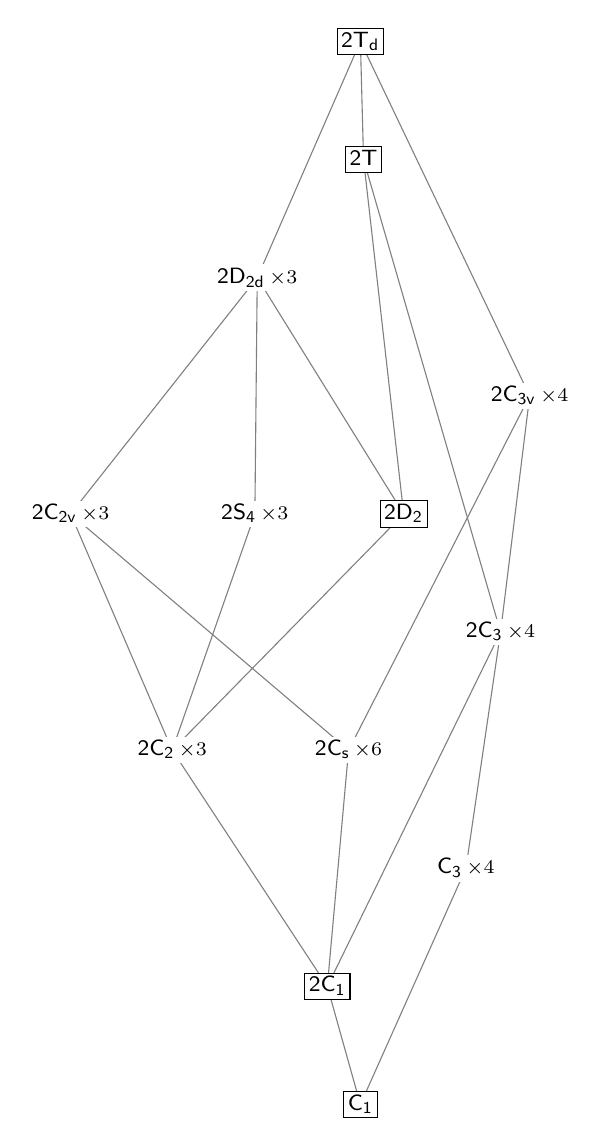
\begin{tikzpicture}[x=1cm, y=1.500cm,
  every node/.style={fill=white, font=\footnotesize, inner xsep=1.5pt, inner ysep=1.2pt, text height=5.6pt, text depth=1.6pt},
  normal/.style={draw, line width=0.4pt}, cover/.style={black!50, line width=0.4pt}]
\draw[cover] (0.00,0) -- (-0.42,1);
\draw[cover] (0.00,0) -- (1.34,2);
\draw[cover] (-0.42,1) -- (-2.39,3);
\draw[cover] (-0.42,1) -- (-0.15,3);
\draw[cover] (-0.42,1) -- (1.78,4);
\draw[cover] (1.34,2) -- (1.78,4);
\draw[cover] (-2.39,3) -- (0.55,5);
\draw[cover] (-2.39,3) -- (-1.34,5);
\draw[cover] (-2.39,3) -- (-3.68,5);
\draw[cover] (-0.15,3) -- (-3.68,5);
\draw[cover] (-0.15,3) -- (2.15,6);
\draw[cover] (1.78,4) -- (2.15,6);
\draw[cover] (1.78,4) -- (0.04,8);
\draw[cover] (0.55,5) -- (-1.31,7);
\draw[cover] (0.55,5) -- (0.04,8);
\draw[cover] (-1.34,5) -- (-1.31,7);
\draw[cover] (-3.68,5) -- (-1.31,7);
\draw[cover] (2.15,6) -- (0.00,9);
\draw[cover] (-1.31,7) -- (0.00,9);
\draw[cover] (0.04,8) -- (0.00,9);
\node[normal] (n00) at (0.00,0) {$\grp{C_{1}}$};
\node[normal] (n01) at (-0.42,1) {$\grp{2C_{1}}$};
\node (n02) at (1.34,2) {$\grp{C_{3}}$\,\nconj{4}};
\node (n03) at (-2.39,3) {$\grp{2C_{2}}$\,\nconj{3}};
\node (n04) at (-0.15,3) {$\grp{2C_{s}}$\,\nconj{6}};
\node (n05) at (1.78,4) {$\grp{2C_{3}}$\,\nconj{4}};
\node[normal] (n06) at (0.55,5) {$\grp{2D_{2}}$};
\node (n07) at (-1.34,5) {$\grp{2S_{4}}$\,\nconj{3}};
\node (n08) at (-3.68,5) {$\grp{2C_{2v}}$\,\nconj{3}};
\node (n09) at (2.15,6) {$\grp{2C_{3v}}$\,\nconj{4}};
\node (n10) at (-1.31,7) {$\grp{2D_{2d}}$\,\nconj{3}};
\node[normal] (n11) at (0.04,8) {$\grp{2T}$};
\node[normal] (n12) at (0.00,9) {$\grp{2T_{d}}$};
\end{tikzpicture}
\end{center}
{\small\setlength{\fillwidth}{\textwidth}\addtolength{\fillwidth}{-12\tabcolsep}\setlength{\colwidth}{0pt}\cellmax{$\grp{2C_{2v}}$ $\samecls$ $\grp{2D_{1h}}$}\cellmax{$\grp{2C_{s}}$ $\samecls$ $\grp{2C_{1h}}$}\cellmax{$\grp{2C_{2}}$ $\samecls$ $\grp{2D_{1}}$}\cellmax{subgrp}\cellmax{$\grp{2C_{3v}}$}\cellmax{$\grp{2D_{2d}}$}\cellmax{$\grp{2C_{1}}$}\cellmax{$\grp{2C_{3}}$}\cellmax{$\grp{2D_{2}}$}\cellmax{$\grp{2S_{4}}$}\cellmax{$\grp{2T_{d}}$}\cellmax{$\grp{2T}$}\cellmax{$\grp{C_{1}}$}\cellmax{$\grp{C_{3}}$}\addtolength{\fillwidth}{-\colwidth}\setlength{\colwidth}{0pt}\cellmax{order}\cellmax{12}\cellmax{16}\cellmax{24}\cellmax{48}\cellmax{1}\cellmax{2}\cellmax{3}\cellmax{4}\cellmax{6}\cellmax{8}\addtolength{\fillwidth}{-\colwidth}\setlength{\colwidth}{0pt}\cellmax{conjugates}\cellmax{1}\cellmax{3}\cellmax{4}\cellmax{6}\addtolength{\fillwidth}{-\colwidth}\setlength{\colwidth}{0pt}\cellmax{normal}\cellmax{yes}\cellmax{no}\addtolength{\fillwidth}{-\colwidth}\setlength{\colwidth}{0pt}\cellmax{$\grp{N}_{\hairsp \grp{2T_{d}}}(\grp{H})$}\cellmax{$\grp{2C_{2v}}$}\cellmax{$\grp{2C_{3v}}$}\cellmax{$\grp{2D_{2d}}$}\cellmax{$\grp{2T_{d}}$}\addtolength{\fillwidth}{-\colwidth}\setlength{\colwidth}{0pt}\cellmax{$\grp{C}_{\hairsp \grp{2T_{d}}}(\grp{H})$}\cellmax{$\grp{2C_{1}}$}\cellmax{$\grp{2C_{3}}$}\cellmax{$\grp{2C_{s}}$}\cellmax{$\grp{2S_{4}}$}\cellmax{$\grp{2T_{d}}$}\addtolength{\fillwidth}{-\colwidth}\setlength{\colwidth}{0pt}\cellmax{$\cls{\barred{E}}$, $\cls{6C_{2}}$, $\cls{6S_{4}}$, $\cls{6\barred{S}_{4}}$, $\cls{12\sigma_{d}}$}\cellmax{$\cls{\barred{E}}$, $\cls{8C_{3}}$, $\cls{8\barred{C}_{3}}$, $\cls{12\sigma_{d}}$}\cellmax{$\cls{\barred{E}}$, $\cls{6C_{2}}$, $\cls{6S_{4}}$, $\cls{6\barred{S}_{4}}$}\cellmax{$\cls{\barred{E}}$, $\cls{8C_{3}}$, $\cls{8\barred{C}_{3}}$, $\cls{6C_{2}}$}\cellmax{$\cls{\barred{E}}$, $\cls{6C_{2}}$, $\cls{12\sigma_{d}}$}\cellmax{$\cls{\barred{E}}$, $\cls{8C_{3}}$, $\cls{8\barred{C}_{3}}$}\cellmax{$\cls{\barred{E}}$, $\cls{12\sigma_{d}}$}\cellmax{classes}\cellmax{$\cls{\barred{E}}$, $\cls{6C_{2}}$}\cellmax{$\cls{8\barred{C}_{3}}$}\cellmax{---}\cellmax{all}\cellmax{$\cls{\barred{E}}$}\fillcap\begin{longtable}{@{}lrrlll>{\RaggedRight\arraybackslash}p{\fillwidth}@{}}\toprule
subgrp & order & conjugates & normal & $\grp{N}_{\hairsp \grp{2T_{d}}}(\grp{H})$ & $\grp{C}_{\hairsp \grp{2T_{d}}}(\grp{H})$ & classes\\\midrule\endhead
\bottomrule\endfoot\endlastfoot
\href{C1.pdf}{$\grp{C_{1}}$} & 1 & 1 & yes & \href{2Td.pdf}{$\grp{2T_{d}}$} & \href{2Td.pdf}{$\grp{2T_{d}}$} & ---\\*
\href{2C1.pdf}{$\grp{2C_{1}}$} & 2 & 1 & yes & \href{2Td.pdf}{$\grp{2T_{d}}$} & \href{2Td.pdf}{$\grp{2T_{d}}$} & $\cls{\barred{E}}$\\
\href{C3.pdf}{$\grp{C_{3}}$} & 3 & 4 & no & \href{2C3v.pdf}{$\grp{2C_{3v}}$} & \href{2C3.pdf}{$\grp{2C_{3}}$} & $\cls{8\barred{C}_{3}}$\\
\href{2C2.pdf}{$\grp{2C_{2}}$} $\samecls$ \href{2D1.pdf}{$\grp{2D_{1}}$} & 4 & 3 & no & \href{2D2d.pdf}{$\grp{2D_{2d}}$} & \href{2S4.pdf}{$\grp{2S_{4}}$} & $\cls{\barred{E}}$, $\cls{6C_{2}}$\\
\href{2C1v.pdf}{$\grp{2C_{s}}$} $\samecls$ \href{2C1h.pdf}{$\grp{2C_{1h}}$} & 4 & 6 & no & \href{2C2v.pdf}{$\grp{2C_{2v}}$} & \href{2C1v.pdf}{$\grp{2C_{s}}$} & $\cls{\barred{E}}$, $\cls{12\sigma_{d}}$\\
\href{2C3.pdf}{$\grp{2C_{3}}$} & 6 & 4 & no & \href{2C3v.pdf}{$\grp{2C_{3v}}$} & \href{2C3.pdf}{$\grp{2C_{3}}$} & $\cls{\barred{E}}$, $\cls{8C_{3}}$, $\cls{8\barred{C}_{3}}$\\
\href{2S4.pdf}{$\grp{2S_{4}}$} & 8 & 3 & no & \href{2D2d.pdf}{$\grp{2D_{2d}}$} & \href{2S4.pdf}{$\grp{2S_{4}}$} & $\cls{\barred{E}}$, $\cls{6C_{2}}$, $\cls{6S_{4}}$, $\cls{6\barred{S}_{4}}$\\
\href{2C2v.pdf}{$\grp{2C_{2v}}$} $\samecls$ \href{2D1h.pdf}{$\grp{2D_{1h}}$} & 8 & 3 & no & \href{2D2d.pdf}{$\grp{2D_{2d}}$} & \href{2C1.pdf}{$\grp{2C_{1}}$} & $\cls{\barred{E}}$, $\cls{6C_{2}}$, $\cls{12\sigma_{d}}$\\
\href{2D2.pdf}{$\grp{2D_{2}}$} & 8 & 1 & yes & \href{2Td.pdf}{$\grp{2T_{d}}$} & \href{2C1.pdf}{$\grp{2C_{1}}$} & $\cls{\barred{E}}$, $\cls{6C_{2}}$\\
\href{2C3v.pdf}{$\grp{2C_{3v}}$} & 12 & 4 & no & \href{2C3v.pdf}{$\grp{2C_{3v}}$} & \href{2C1.pdf}{$\grp{2C_{1}}$} & $\cls{\barred{E}}$, $\cls{8C_{3}}$, $\cls{8\barred{C}_{3}}$, $\cls{12\sigma_{d}}$\\
\href{2D2d.pdf}{$\grp{2D_{2d}}$} & 16 & 3 & no & \href{2D2d.pdf}{$\grp{2D_{2d}}$} & \href{2C1.pdf}{$\grp{2C_{1}}$} & $\cls{\barred{E}}$, $\cls{6C_{2}}$, $\cls{6S_{4}}$, $\cls{6\barred{S}_{4}}$, $\cls{12\sigma_{d}}$\\
\href{2T.pdf}{$\grp{2T}$} & 24 & 1 & yes & \href{2Td.pdf}{$\grp{2T_{d}}$} & \href{2C1.pdf}{$\grp{2C_{1}}$} & $\cls{\barred{E}}$, $\cls{8C_{3}}$, $\cls{8\barred{C}_{3}}$, $\cls{6C_{2}}$\\*
\href{2Td.pdf}{$\grp{2T_{d}}$} & 48 & 1 & yes & \href{2Td.pdf}{$\grp{2T_{d}}$} & \href{2C1.pdf}{$\grp{2C_{1}}$} & all\\
\bottomrule\end{longtable}}
\needspace{103pt}
\section{Descent of symmetry}\label{s:subduction}
Conventions: \href{../../CONVENTIONS.pdf}{CONVENTIONS.pdf}, sections \href{../../../rotation/CONVENTIONS.pdf\#conv.12.2}{12.2}, \href{../../../rotation/CONVENTIONS.pdf\#conv.12.4}{12.4} and \href{../../CONVENTIONS.pdf\#conv.28}{28}.
A column is a class of subgroups $\grp{H}$, in the order of the table of section~\ref{s:subgroups}. The row subgrp names it by its symbol, as in that table. The symbol links to the document of $\grp{H}$. The entry of row $\Gamma$ is $\restr{\Gamma}{\grp{H}}$, the restriction of $\Gamma$ along a monomorphism from the record of $\grp{H}$ onto the subgroup, as a sum of the irreps of $\grp{H}$. The monomorphism identifies the subgroup with its record, and $\grp{H}$ names both. The rows of the vector irreps of a preimage are those of \href{../../../rotation/data/pdf/Td.pdf}{$\grp{T_{d}}$} (\texttt{vector\symbol{95}subduction}). The column of a section, which the record does not store, is that of its preimage with the spinor irreps renamed (\href{../../CONVENTIONS.pdf}{CONVENTIONS.pdf}, section \href{../../CONVENTIONS.pdf\#conv.27}{27}).
{\small\begin{longtable}{@{}lccccc@{}}\toprule
subgrp & \href{2C1.pdf}{$\grp{2C_{1}}$} & \href{C3.pdf}{$\grp{C_{3}}$} & \href{2C2.pdf}{$\grp{2C_{2}}$} & \href{2C1v.pdf}{$\grp{2C_{s}}$} & \href{2C3.pdf}{$\grp{2C_{3}}$}\\\midrule\endhead
\bottomrule\endfoot\endlastfoot
$\irr{a}_{1}$ & $\irr{a}$ & $\irr{a}$ & $\irr{a}$ & $\irr{a}'$ & $\irr{a}$\\*
$\irr{a}_{2}$ & $\irr{a}$ & $\irr{a}$ & $\irr{a}$ & $\irr{a}''$ & $\irr{a}$\\*
$\irr{e}$ & $2\,\irr{a}$ & $\conjpair{1}\irr{e}\oplus \conjpair{2}\irr{e}$ & $2\,\irr{a}$ & $\irr{a}'\oplus \irr{a}''$ & $\conjpair{1}\irr{e}\oplus \conjpair{2}\irr{e}$\\*
$\irr{t}_{1}$ & $3\,\irr{a}$ & $\irr{a}\oplus \conjpair{1}\irr{e}\oplus \conjpair{2}\irr{e}$ & $\irr{a}\oplus 2\,\irr{b}$ & $\irr{a}'\oplus 2\,\irr{a}''$ & $\irr{a}\oplus \conjpair{1}\irr{e}\oplus \conjpair{2}\irr{e}$\\*
$\irr{t}_{2}$ & $3\,\irr{a}$ & $\irr{a}\oplus \conjpair{1}\irr{e}\oplus \conjpair{2}\irr{e}$ & $\irr{a}\oplus 2\,\irr{b}$ & $2\,\irr{a}'\oplus \irr{a}''$ & $\irr{a}\oplus \conjpair{1}\irr{e}\oplus \conjpair{2}\irr{e}$\\*
$\irr{e}_{1/2}$ & $2\,\irr{a}_{1/2}$ & $\conjpair{2}\irr{e}\oplus \conjpair{1}\irr{e}$ & $\conjpair{1}\irr{e}_{1/2}\oplus \conjpair{2}\irr{e}_{1/2}$ & $\conjpair{1}\irr{e}_{1/2}\oplus \conjpair{2}\irr{e}_{1/2}$ & $\conjpair{1}\irr{e}_{1/2}\oplus \conjpair{2}\irr{e}_{1/2}$\\*
$\irr{e}_{5/2}$ & $2\,\irr{a}_{1/2}$ & $\conjpair{2}\irr{e}\oplus \conjpair{1}\irr{e}$ & $\conjpair{1}\irr{e}_{1/2}\oplus \conjpair{2}\irr{e}_{1/2}$ & $\conjpair{1}\irr{e}_{1/2}\oplus \conjpair{2}\irr{e}_{1/2}$ & $\conjpair{1}\irr{e}_{1/2}\oplus \conjpair{2}\irr{e}_{1/2}$\\*
$\irr{g}_{3/2}$ & $4\,\irr{a}_{1/2}$ & $2\,\irr{a}\oplus \conjpair{2}\irr{e}\oplus \conjpair{1}\irr{e}$ & $2\,\conjpair{1}\irr{e}_{1/2}\oplus 2\,\conjpair{2}\irr{e}_{1/2}$ & $2\,\conjpair{1}\irr{e}_{1/2}\oplus 2\,\conjpair{2}\irr{e}_{1/2}$ & $2\,\irr{a}_{3/2}\oplus \conjpair{1}\irr{e}_{1/2}\oplus \conjpair{2}\irr{e}_{1/2}$\\
\bottomrule\end{longtable}}
{\small\begin{longtable}{@{}lcccc@{}}\toprule
subgrp & \href{2S4.pdf}{$\grp{2S_{4}}$} & \href{2C2v.pdf}{$\grp{2C_{2v}}$} & \href{2D2.pdf}{$\grp{2D_{2}}$} & \href{2C3v.pdf}{$\grp{2C_{3v}}$}\\\midrule\endhead
\bottomrule\endfoot\endlastfoot
$\irr{a}_{1}$ & $\irr{a}$ & $\irr{a}_{1}$ & $\irr{a}$ & $\irr{a}_{1}$\\*
$\irr{a}_{2}$ & $\irr{b}$ & $\irr{a}_{2}$ & $\irr{a}$ & $\irr{a}_{2}$\\*
$\irr{e}$ & $\irr{a}\oplus \irr{b}$ & $\irr{a}_{1}\oplus \irr{a}_{2}$ & $2\,\irr{a}$ & $\irr{e}$\\*
$\irr{t}_{1}$ & $\irr{a}\oplus \conjpair{1}\irr{e}\oplus \conjpair{2}\irr{e}$ & $\irr{a}_{2}\oplus \irr{b}_{1}\oplus \irr{b}_{2}$ & $\irr{b}_{1}\oplus \irr{b}_{2}\oplus \irr{b}_{3}$ & $\irr{a}_{2}\oplus \irr{e}$\\*
$\irr{t}_{2}$ & $\irr{b}\oplus \conjpair{1}\irr{e}\oplus \conjpair{2}\irr{e}$ & $\irr{a}_{1}\oplus \irr{b}_{1}\oplus \irr{b}_{2}$ & $\irr{b}_{1}\oplus \irr{b}_{2}\oplus \irr{b}_{3}$ & $\irr{a}_{1}\oplus \irr{e}$\\*
$\irr{e}_{1/2}$ & $\conjpair{1}\irr{e}_{1/2}\oplus \conjpair{2}\irr{e}_{1/2}$ & $\irr{e}_{1/2}$ & $\irr{e}_{1/2}$ & $\irr{e}_{1/2}$\\*
$\irr{e}_{5/2}$ & $\conjpair{1}\irr{e}_{3/2}\oplus \conjpair{2}\irr{e}_{3/2}$ & $\irr{e}_{1/2}$ & $\irr{e}_{1/2}$ & $\irr{e}_{1/2}$\\*
$\irr{g}_{3/2}$ & $\conjpair{1}\irr{e}_{1/2}\oplus \conjpair{2}\irr{e}_{1/2}\oplus \conjpair{1}\irr{e}_{3/2}\oplus \conjpair{2}\irr{e}_{3/2}$ & $2\,\irr{e}_{1/2}$ & $2\,\irr{e}_{1/2}$ & $\irr{e}_{1/2}\oplus \conjpair{1}\irr{e}_{3/2}\oplus \conjpair{2}\irr{e}_{3/2}$\\
\bottomrule\end{longtable}}
{\small\begin{longtable}{@{}lcc@{}}\toprule
subgrp & \href{2D2d.pdf}{$\grp{2D_{2d}}$} & \href{2T.pdf}{$\grp{2T}$}\\\midrule\endhead
\bottomrule\endfoot\endlastfoot
$\irr{a}_{1}$ & $\irr{a}_{1}$ & $\irr{a}$\\*
$\irr{a}_{2}$ & $\irr{b}_{1}$ & $\irr{a}$\\*
$\irr{e}$ & $\irr{a}_{1}\oplus \irr{b}_{1}$ & $\conjpair{1}\irr{e}\oplus \conjpair{2}\irr{e}$\\*
$\irr{t}_{1}$ & $\irr{a}_{2}\oplus \irr{e}$ & $\irr{t}$\\*
$\irr{t}_{2}$ & $\irr{b}_{2}\oplus \irr{e}$ & $\irr{t}$\\*
$\irr{e}_{1/2}$ & $\irr{e}_{1/2}$ & $\irr{e}_{1/2}$\\*
$\irr{e}_{5/2}$ & $\irr{e}_{3/2}$ & $\irr{e}_{1/2}$\\*
$\irr{g}_{3/2}$ & $\irr{e}_{1/2}\oplus \irr{e}_{3/2}$ & $\conjpair{1}\irr{g}_{3/2}\oplus \conjpair{2}\irr{g}_{3/2}$\\
\bottomrule\end{longtable}}
\leavevmode\label{n:irrep.Delta}Read down a column, a table gives induction (Frobenius reciprocity): $\Gamma$ occurs in $\Ind{\grp{H}}{\grp{2T_{d}}} \Lambda$ as often as $\Lambda$ occurs in the entry of row $\Gamma$. For every entry of a spinor irrep, the record holds the unitary matrix that carries $\restr{\Gamma}{\grp{H}}$ into the direct sum of the matrices of $\grp{H}$ (\texttt{subduction[].blocks}). For every class $\grp{H}$ it holds the left coset representatives (\texttt{transversal}). From both, $\Ind{\grp{H}}{\grp{2T_{d}}} \Lambda$ and its intertwiners follow as in \href{../../CONVENTIONS.pdf}{CONVENTIONS.pdf}, section \href{../../../rotation/CONVENTIONS.pdf\#conv.12.4}{12.4}.
\needspace{190pt}
\partbox{Angular momentum}
\section{Subduction from \texorpdfstring{$\grp{Pin^{-}(3)}$}{Pin\unichar{8315}(3)}}\label{s:subduction_parent}
Conventions: \href{../../CONVENTIONS.pdf}{CONVENTIONS.pdf}, sections \href{../../../rotation/CONVENTIONS.pdf\#conv.11}{11} and \href{../../CONVENTIONS.pdf\#conv.25.1}{25.1}.
\leavevmode\label{n:index.J}\label{n:index.parity}\label{n:irrep.o3}The irrep $\irrJp{J}{p}$ of $\grp{Pin^{-}(3)}$ has angular momentum $J$ ($J = 0, \nicefrac{1}{2}, 1, \dots$) and parity $p = \pm 1$. An element $(U, \varepsilon)$ acts on it as $\varepsilon^{[p = -1]}$ times $U$ acting on the kets of angular momentum $J$, and $\elt{\barred{E}}$ as $(-1)^{2J}$. \label{n:function.character.parent}\label{n:function.multiplicity}An element whose $\grp{SU(2)}$ part is $\lift{R}_{\vv}(\omega)$ (section~\ref{s:elements}) has the character
\begin{equation}\label{e:chi}\chi^{(J,p)}(g) = p^{\iverson{\det g = -1}}\sum_{m=-J}^{J} \expe^{\iunit m\omega},\end{equation}
and $b_\Gamma(J, p)$ is the multiplicity of $\Gamma$ in
\begin{equation}\label{e:parent}\restr{\irrJp{J}{p}}{\grp{2T_{d}}}.\end{equation}
At integer $J$ only the vector irreps occur, and $b_\Gamma(J, p)$ is the multiplicity in the subduction from $\grp{O(3)}$ to \href{../../../rotation/data/pdf/Td.pdf}{$\grp{T_{d}}$} (\texttt{integer\symbol{95}J}). \label{n:index.increment}At half-integer $J$ only the spinor irreps occur: each table gives $b_\Gamma(J, p)$ for $2J \le 41$, and $b_\Gamma(J + 12, p) = b_\Gamma(J, p) + \Delta_\Gamma$ for every $J$, where $\Delta_\Gamma$ is the last row of the table of parity $p$. A table leaves out irreps of multiplicity 0 at every $J$.
\leavevmode\label{n:operator.determinant.character}The determinant exchanges the parities: $\irrJp{J}{-1} = \irrJp{J}{+1} \irrprod \det$, so that $b_\Gamma(J, -1) = b_{\Gamma \irrprod \det_{\grp{2T_{d}}}}(J, +1)$.
\needspace{182pt}
\paragraph{Half-integer $J$, $p = +1$.}
{\small\begin{longtable}{@{}rrrr@{\hspace{18pt}}rrrr@{\hspace{18pt}}rrrr@{}}\toprule
$J$ & $\irr{e}_{1/2}$ & $\irr{e}_{5/2}$ & $\irr{g}_{3/2}$ & $J$ & $\irr{e}_{1/2}$ & $\irr{e}_{5/2}$ & $\irr{g}_{3/2}$ & $J$ & $\irr{e}_{1/2}$ & $\irr{e}_{5/2}$ & $\irr{g}_{3/2}$\\\midrule\endhead
\bottomrule\endfoot\endlastfoot
$\nicefrac{1}{2}$ & 1 & 0 & 0 & $\nicefrac{17}{2}$ & 2 & 1 & 3 & $\nicefrac{33}{2}$ & 3 & 2 & 6\\*
$\nicefrac{3}{2}$ & 0 & 0 & 1 & $\nicefrac{19}{2}$ & 2 & 2 & 3 & $\nicefrac{35}{2}$ & 3 & 3 & 6\\*
$\nicefrac{5}{2}$ & 0 & 1 & 1 & $\nicefrac{21}{2}$ & 1 & 2 & 4 & $\nicefrac{37}{2}$ & 3 & 4 & 6\\*
$\nicefrac{7}{2}$ & 1 & 1 & 1 & $\nicefrac{23}{2}$ & 2 & 2 & 4 & $\nicefrac{39}{2}$ & 3 & 3 & 7\\*
$\nicefrac{9}{2}$ & 1 & 0 & 2 & $\nicefrac{25}{2}$ & 3 & 2 & 4 & $\nicefrac{41}{2}$ & 4 & 3 & 7\\*\noalign{\vskip 1.5pt}\multispan{4} & \multispan{4} & \multispan{4}\leaders\hrule height\cmidrulewidth\hfill\kern0pt\\*\noalign{\vskip 1.5pt}
$\nicefrac{11}{2}$ & 1 & 1 & 2 & $\nicefrac{27}{2}$ & 2 & 2 & 5 & $\Delta_\Gamma$ & 2 & 2 & 4\\*
$\nicefrac{13}{2}$ & 1 & 2 & 2 & $\nicefrac{29}{2}$ & 2 & 3 & 5 &  &  &  & \\*
$\nicefrac{15}{2}$ & 1 & 1 & 3 & $\nicefrac{31}{2}$ & 3 & 3 & 5 &  &  &  & \\
\bottomrule\end{longtable}}
\needspace{182pt}
\paragraph{Half-integer $J$, $p = -1$.}
{\small\begin{longtable}{@{}rrrr@{\hspace{18pt}}rrrr@{\hspace{18pt}}rrrr@{}}\toprule
$J$ & $\irr{e}_{1/2}$ & $\irr{e}_{5/2}$ & $\irr{g}_{3/2}$ & $J$ & $\irr{e}_{1/2}$ & $\irr{e}_{5/2}$ & $\irr{g}_{3/2}$ & $J$ & $\irr{e}_{1/2}$ & $\irr{e}_{5/2}$ & $\irr{g}_{3/2}$\\\midrule\endhead
\bottomrule\endfoot\endlastfoot
$\nicefrac{1}{2}$ & 0 & 1 & 0 & $\nicefrac{17}{2}$ & 1 & 2 & 3 & $\nicefrac{33}{2}$ & 2 & 3 & 6\\*
$\nicefrac{3}{2}$ & 0 & 0 & 1 & $\nicefrac{19}{2}$ & 2 & 2 & 3 & $\nicefrac{35}{2}$ & 3 & 3 & 6\\*
$\nicefrac{5}{2}$ & 1 & 0 & 1 & $\nicefrac{21}{2}$ & 2 & 1 & 4 & $\nicefrac{37}{2}$ & 4 & 3 & 6\\*
$\nicefrac{7}{2}$ & 1 & 1 & 1 & $\nicefrac{23}{2}$ & 2 & 2 & 4 & $\nicefrac{39}{2}$ & 3 & 3 & 7\\*
$\nicefrac{9}{2}$ & 0 & 1 & 2 & $\nicefrac{25}{2}$ & 2 & 3 & 4 & $\nicefrac{41}{2}$ & 3 & 4 & 7\\*\noalign{\vskip 1.5pt}\multispan{4} & \multispan{4} & \multispan{4}\leaders\hrule height\cmidrulewidth\hfill\kern0pt\\*\noalign{\vskip 1.5pt}
$\nicefrac{11}{2}$ & 1 & 1 & 2 & $\nicefrac{27}{2}$ & 2 & 2 & 5 & $\Delta_\Gamma$ & 2 & 2 & 4\\*
$\nicefrac{13}{2}$ & 2 & 1 & 2 & $\nicefrac{29}{2}$ & 3 & 2 & 5 &  &  &  & \\*
$\nicefrac{15}{2}$ & 1 & 1 & 3 & $\nicefrac{31}{2}$ & 3 & 3 & 5 &  &  &  & \\
\bottomrule\end{longtable}}
\needspace{110pt}
\section{Multiplicities and allowed \texorpdfstring{$m$}{m}}\label{s:multiplicities}
Conventions: \href{../../CONVENTIONS.pdf}{CONVENTIONS.pdf}, sections \href{../../../rotation/CONVENTIONS.pdf\#conv.14}{14} and \href{../../CONVENTIONS.pdf\#conv.26}{26}.
\leavevmode\label{n:function.generating}\label{n:index.generating.variable}\label{n:function.generating.numerator}The multiplicity $b_\Gamma(J) = b_\Gamma(J, +1)$ is the number of blocks of $\Gamma$ at $J$, with the generating function
\begin{equation}\label{e:gf}H_\Gamma(t) = \sum_{J\ge1/2} b_\Gamma(J)\,t^{2J} = P_\Gamma(t)/((1-t^{6})(1-t^{8})),\end{equation}
summed over the half-integer $J$. The listed residues are the $2m \bmod 8$ of the nonzero components of the vectors of $\Gamma$.
{\small\begin{longtable}{@{}lll@{}}\toprule
$\Gamma$ & $P_\Gamma(t)$ & $2m \bmod 8$\\\midrule\endhead
\bottomrule\endfoot\endlastfoot
$\irr{e}_{1/2}$ & $t + t^{11}$ & 1, 7\\*
$\irr{e}_{5/2}$ & $t^{5} + t^{7}$ & 3, 5\\*
$\irr{g}_{3/2}$ & $t^{3} + t^{5} + t^{7} + t^{9}$ & 1, 3, 5, 7\\
\bottomrule\end{longtable}}
\needspace{122pt}
\section{Symmetry-adapted bases}\label{s:bases}
Conventions: \href{../../CONVENTIONS.pdf}{CONVENTIONS.pdf}, sections \href{../../../rotation/CONVENTIONS.pdf\#conv.14}{14}, \href{../../../rotation/CONVENTIONS.pdf\#conv.14.2}{14.2} and \href{../../CONVENTIONS.pdf\#conv.26}{26}.
\leavevmode\label{n:index.m}\label{n:vector.ket}The bases at integer $J$ are those of \href{../../../rotation/data/pdf/Td.pdf}{$\grp{T_{d}}$} (\texttt{integer\symbol{95}J}), and at half-integer $J$ the kets $\jm{J}{m}$, $m = J, J-1, \dots, -J$, carry $\irrJp{J}{+1}$. \label{n:matrix.wigner}The Wigner matrix $\wignerD{J}$ of $\grp{SU(2)}$ satisfies $\wignerD{1/2}(U) = U$ on $\jm{1/2}{1/2}$, $\jm{1/2}{-1/2}$. The element $g$ of $\grp{2T_{d}}$ whose $\grp{SU(2)}$ part is $U$ acts as
\begin{equation}\label{e:action}g\,\jm{J}{m} = \sum_{m'} \jm{J}{m'}\; \conj{\wignerD{J}_{m m'}(U)},\end{equation}
so $\lift{R}_{z}(\omega)$ multiplies $\jm{J}{m}$ by $\expe^{\iunit m\omega}$, $0 \le \omega < 4\pi$, and $\elt{\barred{E}}$ by $-1$. \label{n:index.ketcoefficient}\label{n:vector.basis.symmetry}\label{n:index.ketweight}\label{n:index.total}A vector is listed by its coefficients $e_m$:
\begin{equation}\label{e:ket}v = \frac{1}{\sqrt{\mathrm{tot}}}\sum_m e_m\sqrt{F_m}\;\jm{J}{m},\qquad F_m = (J+m)!\,(J-m)!,\qquad \mathrm{tot} = \sum_m |e_m|^2F_m;\end{equation}
\leavevmode\label{n:index.factor.c}the amplitude of $\jm{J}{m}$ is $e_m\sqrt{F_m/\mathrm{tot}}$, and a vector written $c\sum_m q_m\jm{J}{m}$ has $e_m = c\,q_m$.
At half-integer $J$ the bases are those of $\grp{2O}$. At the parity $+1$ an element acts on the kets as the element of $\grp{2O}$ with the same $\grp{SU(2)}$ part. Each spinor irrep of $\grp{2O}$ then has the matrices of a spinor irrep of $\grp{2T_{d}}$, as in this table.
\begin{center}\begin{tabular}{@{}ll@{}}\toprule
$\grp{2O}$ & $\grp{2T_{d}}$\\\midrule
$\irr{e}_{1/2}$ & $\irr{e}_{1/2}$\\
$\irr{e}_{5/2}$ & $\irr{e}_{5/2}$\\
$\irr{g}_{3/2}$ & $\irr{g}_{3/2}$\\
\bottomrule\end{tabular}\end{center}
At the parity $p = -1$ a block keeps its kets, and its irrep $\Gamma$ becomes $\Gamma \irrprod \det_{\grp{2T_{d}}}$: $\irr{e}_{1/2} \to \irr{e}_{5/2}$, $\irr{e}_{5/2} \to \irr{e}_{1/2}$.
The bases have 44 blocks and 132 vectors at $J = \nicefrac{1}{2}, \nicefrac{3}{2}, \dots, \nicefrac{21}{2}$. \label{n:head.vector}A row gives a vector of a block at $J$: the block's irrep and copy index $\mult$, the partner index $\intx$ and the vector. The full set $J \le \nicefrac{121}{2}$ (1261 blocks, 3782 vectors) is in \texttt{data/symmetry\symbol{95}adapted\symbol{95}bases/2Td/}. The repository holds $J \le \nicefrac{21}{2}$, and the release archive \texttt{2Td\symbol{95}2J023-2J121.tar} holds $J = \nicefrac{23}{2}, \nicefrac{25}{2}, \dots, \nicefrac{121}{2}$ and unpacks in the folder \texttt{double/} (README.md).
{\small\setlength{\tabcolsep}{3pt}\setlength{\fillwidth}{\textwidth}\addtolength{\fillwidth}{-\dimexpr 6\tabcolsep+4pt\relax}\setlength{\colwidth}{0pt}\cellmax{11/2}\cellmax{13/2}\cellmax{15/2}\cellmax{17/2}\cellmax{19/2}\cellmax{21/2}\cellmax{1/2}\cellmax{3/2}\cellmax{5/2}\cellmax{7/2}\cellmax{9/2}\cellmax{$J$}\addtolength{\fillwidth}{-\colwidth}\setlength{\colwidth}{0pt}\cellmax{$\irr{e}_{1/2}$}\cellmax{$\irr{e}_{5/2}$}\cellmax{$\irr{g}_{3/2}$}\cellmax{irrep}\addtolength{\fillwidth}{-\colwidth}\setlength{\colwidth}{0pt}\cellmax{$\mult$}\cellmax{1}\cellmax{2}\cellmax{3}\cellmax{4}\addtolength{\fillwidth}{-\colwidth}\setlength{\colwidth}{0pt}\cellmax{$\intx$}\cellmax{1}\cellmax{2}\cellmax{3}\cellmax{4}\addtolength{\fillwidth}{-\colwidth}\setlength{\colwidth}{0pt}\cellmax{$-\sqrt{3}\,(37235\,\jm{\nicefrac{21}{2}}{-\nicefrac{15}{2}}$ $-$ $410040\,\jm{\nicefrac{21}{2}}{-\nicefrac{7}{2}}$ $+$ $803998\,\jm{\nicefrac{21}{2}}{\nicefrac{1}{2}}$ $-$ $56032\,\jm{\nicefrac{21}{2}}{\nicefrac{9}{2}}$ $+$ $18055\,\jm{\nicefrac{21}{2}}{\nicefrac{17}{2}})$}\cellmax{$\sqrt{3}\,(18055\,\jm{\nicefrac{21}{2}}{-\nicefrac{17}{2}}$ $-$ $56032\,\jm{\nicefrac{21}{2}}{-\nicefrac{9}{2}}$ $+$ $803998\,\jm{\nicefrac{21}{2}}{-\nicefrac{1}{2}}$ $-$ $410040\,\jm{\nicefrac{21}{2}}{\nicefrac{7}{2}}$ $+$ $37235\,\jm{\nicefrac{21}{2}}{\nicefrac{15}{2}})$}\cellmax{$\sqrt{3}\,(2485\,\jm{\nicefrac{21}{2}}{-\nicefrac{17}{2}}$ $-$ $54264\,\jm{\nicefrac{21}{2}}{-\nicefrac{9}{2}}$ $+$ $58786\,\jm{\nicefrac{21}{2}}{-\nicefrac{1}{2}}$ $+$ $77520\,\jm{\nicefrac{21}{2}}{\nicefrac{7}{2}}$ $-$ $4655\,\jm{\nicefrac{21}{2}}{\nicefrac{15}{2}})$}\cellmax{$-\jm{\nicefrac{21}{2}}{-\nicefrac{21}{2}}$ $-65\,\jm{\nicefrac{21}{2}}{-\nicefrac{13}{2}}$ $-610\,\jm{\nicefrac{21}{2}}{-\nicefrac{5}{2}}$ $+$ $1430\,\jm{\nicefrac{21}{2}}{\nicefrac{3}{2}}$ $+$ $259\,\jm{\nicefrac{21}{2}}{\nicefrac{11}{2}}$ $+$ $11\,\jm{\nicefrac{21}{2}}{\nicefrac{19}{2}}$}\cellmax{$\sqrt{3}\,(4655\,\jm{\nicefrac{21}{2}}{-\nicefrac{15}{2}}$ $-$ $77520\,\jm{\nicefrac{21}{2}}{-\nicefrac{7}{2}}$ $-$ $58786\,\jm{\nicefrac{21}{2}}{\nicefrac{1}{2}}$ $+$ $54264\,\jm{\nicefrac{21}{2}}{\nicefrac{9}{2}}$ $-$ $2485\,\jm{\nicefrac{21}{2}}{\nicefrac{17}{2}})$}\cellmax{$11\,\jm{\nicefrac{21}{2}}{-\nicefrac{19}{2}}$ $+$ $259\,\jm{\nicefrac{21}{2}}{-\nicefrac{11}{2}}$ $+$ $1430\,\jm{\nicefrac{21}{2}}{-\nicefrac{3}{2}}$ $-610\,\jm{\nicefrac{21}{2}}{\nicefrac{5}{2}}$ $-65\,\jm{\nicefrac{21}{2}}{\nicefrac{13}{2}}$ $-\jm{\nicefrac{21}{2}}{\nicefrac{21}{2}}$}\cellmax{$\sqrt{3}\,(23\,\jm{\nicefrac{21}{2}}{-\nicefrac{17}{2}}$ $+$ $8668\,\jm{\nicefrac{21}{2}}{-\nicefrac{9}{2}}$ $+$ $19474\,\jm{\nicefrac{21}{2}}{-\nicefrac{1}{2}}$ $+$ $2092\,\jm{\nicefrac{21}{2}}{\nicefrac{7}{2}}$ $-$ $1073\,\jm{\nicefrac{21}{2}}{\nicefrac{15}{2}})$}\cellmax{$\sqrt{3}\,(1073\,\jm{\nicefrac{21}{2}}{-\nicefrac{15}{2}}$ $-$ $2092\,\jm{\nicefrac{21}{2}}{-\nicefrac{7}{2}}$ $-$ $19474\,\jm{\nicefrac{21}{2}}{\nicefrac{1}{2}}$ $-$ $8668\,\jm{\nicefrac{21}{2}}{\nicefrac{9}{2}}$ $-$ $23\,\jm{\nicefrac{21}{2}}{\nicefrac{17}{2}})$}\cellmax{$3\,\jm{\nicefrac{21}{2}}{-\nicefrac{19}{2}}$ $+$ $99\,\jm{\nicefrac{21}{2}}{-\nicefrac{11}{2}}$ $-730\,\jm{\nicefrac{21}{2}}{-\nicefrac{3}{2}}$ $+$ $126\,\jm{\nicefrac{21}{2}}{\nicefrac{5}{2}}$ $-9\,\jm{\nicefrac{21}{2}}{\nicefrac{13}{2}}$ $-\jm{\nicefrac{21}{2}}{\nicefrac{21}{2}}$}\cellmax{$\jm{\nicefrac{21}{2}}{-\nicefrac{21}{2}}$ $+$ $9\,\jm{\nicefrac{21}{2}}{-\nicefrac{13}{2}}$ $-126\,\jm{\nicefrac{21}{2}}{-\nicefrac{5}{2}}$ $+$ $730\,\jm{\nicefrac{21}{2}}{\nicefrac{3}{2}}$ $-99\,\jm{\nicefrac{21}{2}}{\nicefrac{11}{2}}$ $-3\,\jm{\nicefrac{21}{2}}{\nicefrac{19}{2}}$}\cellmax{$-194\,\jm{\nicefrac{21}{2}}{-\nicefrac{19}{2}}$ $-1657\,\jm{\nicefrac{21}{2}}{-\nicefrac{11}{2}}$ $-29318\,\jm{\nicefrac{21}{2}}{\nicefrac{5}{2}}$ $+$ $2042\,\jm{\nicefrac{21}{2}}{\nicefrac{13}{2}}$ $-57\,\jm{\nicefrac{21}{2}}{\nicefrac{21}{2}}$}\cellmax{$-\sqrt{3}\,(229\,\jm{\nicefrac{17}{2}}{-\nicefrac{15}{2}}$ $+$ $988\,\jm{\nicefrac{17}{2}}{-\nicefrac{7}{2}}$ $-$ $4290\,\jm{\nicefrac{17}{2}}{\nicefrac{1}{2}}$ $-$ $1700\,\jm{\nicefrac{17}{2}}{\nicefrac{9}{2}}$ $+$ $37\,\jm{\nicefrac{17}{2}}{\nicefrac{17}{2}})$}\cellmax{$57\,\jm{\nicefrac{21}{2}}{-\nicefrac{21}{2}}$ $-2042\,\jm{\nicefrac{21}{2}}{-\nicefrac{13}{2}}$ $+$ $29318\,\jm{\nicefrac{21}{2}}{-\nicefrac{5}{2}}$ $+$ $1657\,\jm{\nicefrac{21}{2}}{\nicefrac{11}{2}}$ $+$ $194\,\jm{\nicefrac{21}{2}}{\nicefrac{19}{2}}$}\cellmax{$\sqrt{3}\,(25\,\jm{\nicefrac{19}{2}}{-\nicefrac{17}{2}}$ $-$ $612\,\jm{\nicefrac{19}{2}}{-\nicefrac{9}{2}}$ $+$ $4862\,\jm{\nicefrac{19}{2}}{-\nicefrac{1}{2}}$ $-$ $1428\,\jm{\nicefrac{19}{2}}{\nicefrac{7}{2}}$ $+$ $225\,\jm{\nicefrac{19}{2}}{\nicefrac{15}{2}})$}\cellmax{$\sqrt{3}\,(37\,\jm{\nicefrac{17}{2}}{-\nicefrac{17}{2}}$ $-$ $1700\,\jm{\nicefrac{17}{2}}{-\nicefrac{9}{2}}$ $-$ $4290\,\jm{\nicefrac{17}{2}}{-\nicefrac{1}{2}}$ $+$ $988\,\jm{\nicefrac{17}{2}}{\nicefrac{7}{2}}$ $+$ $229\,\jm{\nicefrac{17}{2}}{\nicefrac{15}{2}})$}\cellmax{$\sqrt{3}\,(225\,\jm{\nicefrac{19}{2}}{-\nicefrac{15}{2}}$ $-$ $1428\,\jm{\nicefrac{19}{2}}{-\nicefrac{7}{2}}$ $+$ $4862\,\jm{\nicefrac{19}{2}}{\nicefrac{1}{2}}$ $-$ $612\,\jm{\nicefrac{19}{2}}{\nicefrac{9}{2}}$ $+$ $25\,\jm{\nicefrac{19}{2}}{\nicefrac{17}{2}})$}\cellmax{$-\sqrt{3}\,(15\,\jm{\nicefrac{19}{2}}{-\nicefrac{17}{2}}$ $-$ $11\,\jm{\nicefrac{19}{2}}{-\nicefrac{9}{2}}$ $-$ $1001\,\jm{\nicefrac{19}{2}}{-\nicefrac{1}{2}}$ $-$ $665\,\jm{\nicefrac{19}{2}}{\nicefrac{7}{2}}$ $-$ $2\,\jm{\nicefrac{19}{2}}{\nicefrac{15}{2}})$}\cellmax{$20\,\jm{\nicefrac{21}{2}}{-\nicefrac{21}{2}}$ $-513\,\jm{\nicefrac{21}{2}}{-\nicefrac{13}{2}}$ $-11628\,\jm{\nicefrac{21}{2}}{-\nicefrac{5}{2}}$ $-8398\,\jm{\nicefrac{21}{2}}{\nicefrac{3}{2}}$ $+$ $39\,\jm{\nicefrac{21}{2}}{\nicefrac{19}{2}}$}\cellmax{$-\sqrt{3}\,(3\,\jm{\nicefrac{21}{2}}{-\nicefrac{17}{2}}$ $-$ $12\,\jm{\nicefrac{21}{2}}{-\nicefrac{9}{2}}$ $-$ $126\,\jm{\nicefrac{21}{2}}{-\nicefrac{1}{2}}$ $-$ $108\,\jm{\nicefrac{21}{2}}{\nicefrac{7}{2}}$ $-$ $13\,\jm{\nicefrac{21}{2}}{\nicefrac{15}{2}})$}\cellmax{$39\,\jm{\nicefrac{21}{2}}{-\nicefrac{19}{2}}$ $-8398\,\jm{\nicefrac{21}{2}}{-\nicefrac{3}{2}}$ $-11628\,\jm{\nicefrac{21}{2}}{\nicefrac{5}{2}}$ $-513\,\jm{\nicefrac{21}{2}}{\nicefrac{13}{2}}$ $+$ $20\,\jm{\nicefrac{21}{2}}{\nicefrac{21}{2}}$}\cellmax{$-\sqrt{3}\,(13\,\jm{\nicefrac{21}{2}}{-\nicefrac{15}{2}}$ $+$ $108\,\jm{\nicefrac{21}{2}}{-\nicefrac{7}{2}}$ $+$ $126\,\jm{\nicefrac{21}{2}}{\nicefrac{1}{2}}$ $+$ $12\,\jm{\nicefrac{21}{2}}{\nicefrac{9}{2}}$ $-$ $3\,\jm{\nicefrac{21}{2}}{\nicefrac{17}{2}})$}\cellmax{$\sqrt{3}\,(2\,\jm{\nicefrac{19}{2}}{-\nicefrac{15}{2}}$ $+$ $665\,\jm{\nicefrac{19}{2}}{-\nicefrac{7}{2}}$ $+$ $1001\,\jm{\nicefrac{19}{2}}{\nicefrac{1}{2}}$ $+$ $11\,\jm{\nicefrac{19}{2}}{\nicefrac{9}{2}}$ $-$ $15\,\jm{\nicefrac{19}{2}}{\nicefrac{17}{2}})$}\cellmax{$-\jm{\nicefrac{19}{2}}{-\nicefrac{19}{2}}$ $+$ $140\,\jm{\nicefrac{19}{2}}{-\nicefrac{11}{2}}$ $-78\,\jm{\nicefrac{19}{2}}{-\nicefrac{3}{2}}$ $+$ $572\,\jm{\nicefrac{19}{2}}{\nicefrac{5}{2}}$ $-121\,\jm{\nicefrac{19}{2}}{\nicefrac{13}{2}}$}\cellmax{$-\sqrt{3}\,(5\,\jm{\nicefrac{19}{2}}{-\nicefrac{15}{2}}$ $-$ $28\,\jm{\nicefrac{19}{2}}{-\nicefrac{7}{2}}$ $-$ $154\,\jm{\nicefrac{19}{2}}{\nicefrac{1}{2}}$ $-$ $76\,\jm{\nicefrac{19}{2}}{\nicefrac{9}{2}}$ $-$ $3\,\jm{\nicefrac{19}{2}}{\nicefrac{17}{2}})$}\cellmax{$-\sqrt{3}\,(\jm{\nicefrac{17}{2}}{-\nicefrac{15}{2}}$ $+$ $364\,\jm{\nicefrac{17}{2}}{-\nicefrac{7}{2}}$ $-$ $858\,\jm{\nicefrac{17}{2}}{\nicefrac{1}{2}}$ $+$ $364\,\jm{\nicefrac{17}{2}}{\nicefrac{9}{2}}$ $+$ $\jm{\nicefrac{17}{2}}{\nicefrac{17}{2}})$}\cellmax{$\sqrt{3}\,(3\,\jm{\nicefrac{19}{2}}{-\nicefrac{17}{2}}$ $+$ $76\,\jm{\nicefrac{19}{2}}{-\nicefrac{9}{2}}$ $+$ $154\,\jm{\nicefrac{19}{2}}{-\nicefrac{1}{2}}$ $+$ $28\,\jm{\nicefrac{19}{2}}{\nicefrac{7}{2}}$ $-$ $5\,\jm{\nicefrac{19}{2}}{\nicefrac{15}{2}})$}\cellmax{$\sqrt{3}\,(\jm{\nicefrac{17}{2}}{-\nicefrac{17}{2}}$ $+$ $364\,\jm{\nicefrac{17}{2}}{-\nicefrac{9}{2}}$ $-$ $858\,\jm{\nicefrac{17}{2}}{-\nicefrac{1}{2}}$ $+$ $364\,\jm{\nicefrac{17}{2}}{\nicefrac{7}{2}}$ $+$ $\jm{\nicefrac{17}{2}}{\nicefrac{15}{2}})$}\cellmax{$-7\,\jm{\nicefrac{19}{2}}{-\nicefrac{17}{2}}$ $+$ $84\,\jm{\nicefrac{19}{2}}{-\nicefrac{9}{2}}$ $+$ $286\,\jm{\nicefrac{19}{2}}{-\nicefrac{1}{2}}$ $-348\,\jm{\nicefrac{19}{2}}{\nicefrac{7}{2}}$ $-15\,\jm{\nicefrac{19}{2}}{\nicefrac{15}{2}}$}\cellmax{$121\,\jm{\nicefrac{19}{2}}{-\nicefrac{13}{2}}$ $-572\,\jm{\nicefrac{19}{2}}{-\nicefrac{5}{2}}$ $+$ $78\,\jm{\nicefrac{19}{2}}{\nicefrac{3}{2}}$ $-140\,\jm{\nicefrac{19}{2}}{\nicefrac{11}{2}}$ $+$ $\jm{\nicefrac{19}{2}}{\nicefrac{19}{2}}$}\cellmax{$-23\,\jm{\nicefrac{19}{2}}{-\nicefrac{13}{2}}$ $-140\,\jm{\nicefrac{19}{2}}{-\nicefrac{5}{2}}$ $+$ $414\,\jm{\nicefrac{19}{2}}{\nicefrac{3}{2}}$ $+$ $4\,\jm{\nicefrac{19}{2}}{\nicefrac{11}{2}}$ $+$ $\jm{\nicefrac{19}{2}}{\nicefrac{19}{2}}$}\cellmax{$15\,\jm{\nicefrac{19}{2}}{-\nicefrac{15}{2}}$ $+$ $348\,\jm{\nicefrac{19}{2}}{-\nicefrac{7}{2}}$ $-286\,\jm{\nicefrac{19}{2}}{\nicefrac{1}{2}}$ $-84\,\jm{\nicefrac{19}{2}}{\nicefrac{9}{2}}$ $+$ $7\,\jm{\nicefrac{19}{2}}{\nicefrac{17}{2}}$}\cellmax{$\jm{\nicefrac{19}{2}}{-\nicefrac{19}{2}}$ $+$ $4\,\jm{\nicefrac{19}{2}}{-\nicefrac{11}{2}}$ $+$ $414\,\jm{\nicefrac{19}{2}}{-\nicefrac{3}{2}}$ $-140\,\jm{\nicefrac{19}{2}}{\nicefrac{5}{2}}$ $-23\,\jm{\nicefrac{19}{2}}{\nicefrac{13}{2}}$}\cellmax{$-7\,\jm{\nicefrac{17}{2}}{-\nicefrac{15}{2}}$ $+$ $212\,\jm{\nicefrac{17}{2}}{-\nicefrac{7}{2}}$ $+$ $110\,\jm{\nicefrac{17}{2}}{\nicefrac{1}{2}}$ $-60\,\jm{\nicefrac{17}{2}}{\nicefrac{9}{2}}$ $+$ $\jm{\nicefrac{17}{2}}{\nicefrac{17}{2}}$}\cellmax{$\jm{\nicefrac{17}{2}}{-\nicefrac{17}{2}}$ $-60\,\jm{\nicefrac{17}{2}}{-\nicefrac{9}{2}}$ $+$ $110\,\jm{\nicefrac{17}{2}}{-\nicefrac{1}{2}}$ $+$ $212\,\jm{\nicefrac{17}{2}}{\nicefrac{7}{2}}$ $-7\,\jm{\nicefrac{17}{2}}{\nicefrac{15}{2}}$}\cellmax{$-475\,\jm{\nicefrac{21}{2}}{-\nicefrac{19}{2}}$ $-7004\,\jm{\nicefrac{21}{2}}{-\nicefrac{11}{2}}$ $-25225\,\jm{\nicefrac{21}{2}}{\nicefrac{13}{2}}$ $-64\,\jm{\nicefrac{21}{2}}{\nicefrac{21}{2}}$}\cellmax{$64\,\jm{\nicefrac{21}{2}}{-\nicefrac{21}{2}}$ $+$ $25225\,\jm{\nicefrac{21}{2}}{-\nicefrac{13}{2}}$ $+$ $7004\,\jm{\nicefrac{21}{2}}{\nicefrac{11}{2}}$ $+$ $475\,\jm{\nicefrac{21}{2}}{\nicefrac{19}{2}}$}\cellmax{$\jm{\nicefrac{21}{2}}{-\nicefrac{17}{2}}$ $+$ $12\,\jm{\nicefrac{21}{2}}{-\nicefrac{9}{2}}$ $-26\,\jm{\nicefrac{21}{2}}{-\nicefrac{1}{2}}$ $+$ $12\,\jm{\nicefrac{21}{2}}{\nicefrac{7}{2}}$ $+$ $\jm{\nicefrac{21}{2}}{\nicefrac{15}{2}}$}\cellmax{$\jm{\nicefrac{21}{2}}{-\nicefrac{15}{2}}$ $+$ $12\,\jm{\nicefrac{21}{2}}{-\nicefrac{7}{2}}$ $-26\,\jm{\nicefrac{21}{2}}{\nicefrac{1}{2}}$ $+$ $12\,\jm{\nicefrac{21}{2}}{\nicefrac{9}{2}}$ $+$ $\jm{\nicefrac{21}{2}}{\nicefrac{17}{2}}$}\cellmax{$\sqrt{3}\,(11\,\jm{\nicefrac{15}{2}}{-\nicefrac{15}{2}}$ $-$ $645\,\jm{\nicefrac{15}{2}}{-\nicefrac{7}{2}}$ $-$ $495\,\jm{\nicefrac{15}{2}}{\nicefrac{1}{2}}$ $+$ $425\,\jm{\nicefrac{15}{2}}{\nicefrac{9}{2}})$}\cellmax{$\sqrt{3}\,(425\,\jm{\nicefrac{15}{2}}{-\nicefrac{9}{2}}$ $-$ $495\,\jm{\nicefrac{15}{2}}{-\nicefrac{1}{2}}$ $-$ $645\,\jm{\nicefrac{15}{2}}{\nicefrac{7}{2}}$ $+$ $11\,\jm{\nicefrac{15}{2}}{\nicefrac{15}{2}})$}\cellmax{$115\,\jm{\nicefrac{19}{2}}{-\nicefrac{13}{2}}$ $+$ $3562\,\jm{\nicefrac{19}{2}}{-\nicefrac{5}{2}}$ $-362\,\jm{\nicefrac{19}{2}}{\nicefrac{11}{2}}$ $+$ $13\,\jm{\nicefrac{19}{2}}{\nicefrac{19}{2}}$}\cellmax{$13\,\jm{\nicefrac{19}{2}}{-\nicefrac{19}{2}}$ $-362\,\jm{\nicefrac{19}{2}}{-\nicefrac{11}{2}}$ $+$ $3562\,\jm{\nicefrac{19}{2}}{\nicefrac{5}{2}}$ $+$ $115\,\jm{\nicefrac{19}{2}}{\nicefrac{13}{2}}$}\cellmax{$23\,\jm{\nicefrac{17}{2}}{-\nicefrac{17}{2}}$ $+$ $952\,\jm{\nicefrac{17}{2}}{-\nicefrac{9}{2}}$ $+$ $4862\,\jm{\nicefrac{17}{2}}{-\nicefrac{1}{2}}$ $+$ $51\,\jm{\nicefrac{17}{2}}{\nicefrac{15}{2}}$}\cellmax{$\sqrt{3}\,(91\,\jm{\nicefrac{15}{2}}{-\nicefrac{9}{2}}$ $-$ $429\,\jm{\nicefrac{15}{2}}{-\nicefrac{1}{2}}$ $+$ $273\,\jm{\nicefrac{15}{2}}{\nicefrac{7}{2}}$ $+$ $\jm{\nicefrac{15}{2}}{\nicefrac{15}{2}})$}\cellmax{$\sqrt{3}\,(\jm{\nicefrac{15}{2}}{-\nicefrac{15}{2}}$ $+$ $273\,\jm{\nicefrac{15}{2}}{-\nicefrac{7}{2}}$ $-$ $429\,\jm{\nicefrac{15}{2}}{\nicefrac{1}{2}}$ $+$ $91\,\jm{\nicefrac{15}{2}}{\nicefrac{9}{2}})$}\cellmax{$51\,\jm{\nicefrac{17}{2}}{-\nicefrac{15}{2}}$ $+$ $4862\,\jm{\nicefrac{17}{2}}{\nicefrac{1}{2}}$ $+$ $952\,\jm{\nicefrac{17}{2}}{\nicefrac{9}{2}}$ $+$ $23\,\jm{\nicefrac{17}{2}}{\nicefrac{17}{2}}$}\cellmax{$5\,\jm{\nicefrac{19}{2}}{-\nicefrac{17}{2}}$ $-408\,\jm{\nicefrac{19}{2}}{-\nicefrac{9}{2}}$ $+$ $442\,\jm{\nicefrac{19}{2}}{-\nicefrac{1}{2}}$ $-39\,\jm{\nicefrac{19}{2}}{\nicefrac{15}{2}}$}\cellmax{$-\sqrt{3}\,(17\,\jm{\nicefrac{15}{2}}{-\nicefrac{9}{2}}$ $+$ $45\,\jm{\nicefrac{15}{2}}{-\nicefrac{1}{2}}$ $+$ $3\,\jm{\nicefrac{15}{2}}{\nicefrac{7}{2}}$ $-$ $\jm{\nicefrac{15}{2}}{\nicefrac{15}{2}})$}\cellmax{$\sqrt{3}\,(3\,\jm{\nicefrac{17}{2}}{-\nicefrac{15}{2}}$ $+$ $56\,\jm{\nicefrac{17}{2}}{-\nicefrac{7}{2}}$ $+$ $70\,\jm{\nicefrac{17}{2}}{\nicefrac{1}{2}}$ $-$ $\jm{\nicefrac{17}{2}}{\nicefrac{17}{2}})$}\cellmax{$\sqrt{3}\,(\jm{\nicefrac{17}{2}}{-\nicefrac{17}{2}}$ $-$ $70\,\jm{\nicefrac{17}{2}}{-\nicefrac{1}{2}}$ $-$ $56\,\jm{\nicefrac{17}{2}}{\nicefrac{7}{2}}$ $-$ $3\,\jm{\nicefrac{17}{2}}{\nicefrac{15}{2}})$}\cellmax{$19\,\jm{\nicefrac{19}{2}}{-\nicefrac{13}{2}}$ $+$ $152\,\jm{\nicefrac{19}{2}}{-\nicefrac{5}{2}}$ $+$ $342\,\jm{\nicefrac{19}{2}}{\nicefrac{3}{2}}$ $-\jm{\nicefrac{19}{2}}{\nicefrac{19}{2}}$}\cellmax{$39\,\jm{\nicefrac{19}{2}}{-\nicefrac{15}{2}}$ $-442\,\jm{\nicefrac{19}{2}}{\nicefrac{1}{2}}$ $+$ $408\,\jm{\nicefrac{19}{2}}{\nicefrac{9}{2}}$ $-5\,\jm{\nicefrac{19}{2}}{\nicefrac{17}{2}}$}\cellmax{$\jm{\nicefrac{19}{2}}{-\nicefrac{19}{2}}$ $-342\,\jm{\nicefrac{19}{2}}{-\nicefrac{3}{2}}$ $-152\,\jm{\nicefrac{19}{2}}{\nicefrac{5}{2}}$ $-19\,\jm{\nicefrac{19}{2}}{\nicefrac{13}{2}}$}\cellmax{$\sqrt{3}\,(\jm{\nicefrac{15}{2}}{-\nicefrac{15}{2}}$ $-$ $3\,\jm{\nicefrac{15}{2}}{-\nicefrac{7}{2}}$ $-$ $45\,\jm{\nicefrac{15}{2}}{\nicefrac{1}{2}}$ $-$ $17\,\jm{\nicefrac{15}{2}}{\nicefrac{9}{2}})$}\cellmax{$-5\,\jm{\nicefrac{13}{2}}{-\nicefrac{11}{2}}$ $+$ $9\,\jm{\nicefrac{13}{2}}{-\nicefrac{3}{2}}$ $-35\,\jm{\nicefrac{13}{2}}{\nicefrac{5}{2}}$ $-\jm{\nicefrac{13}{2}}{\nicefrac{13}{2}}$}\cellmax{$-5\,\jm{\nicefrac{17}{2}}{-\nicefrac{11}{2}}$ $-85\,\jm{\nicefrac{17}{2}}{-\nicefrac{3}{2}}$ $-7\,\jm{\nicefrac{17}{2}}{\nicefrac{5}{2}}$ $+$ $\jm{\nicefrac{17}{2}}{\nicefrac{13}{2}}$}\cellmax{$-7\,\jm{\nicefrac{15}{2}}{-\nicefrac{9}{2}}$ $-99\,\jm{\nicefrac{15}{2}}{-\nicefrac{1}{2}}$ $-21\,\jm{\nicefrac{15}{2}}{\nicefrac{7}{2}}$ $-\jm{\nicefrac{15}{2}}{\nicefrac{15}{2}}$}\cellmax{$-\jm{\nicefrac{13}{2}}{-\nicefrac{13}{2}}$ $+$ $5\,\jm{\nicefrac{13}{2}}{-\nicefrac{5}{2}}$ $+$ $57\,\jm{\nicefrac{13}{2}}{\nicefrac{3}{2}}$ $+$ $3\,\jm{\nicefrac{13}{2}}{\nicefrac{11}{2}}$}\cellmax{$-\jm{\nicefrac{15}{2}}{-\nicefrac{11}{2}}$ $+$ $51\,\jm{\nicefrac{15}{2}}{-\nicefrac{3}{2}}$ $+$ $13\,\jm{\nicefrac{15}{2}}{\nicefrac{5}{2}}$ $+$ $\jm{\nicefrac{15}{2}}{\nicefrac{13}{2}}$}\cellmax{$-\jm{\nicefrac{17}{2}}{-\nicefrac{13}{2}}$ $+$ $7\,\jm{\nicefrac{17}{2}}{-\nicefrac{5}{2}}$ $+$ $85\,\jm{\nicefrac{17}{2}}{\nicefrac{3}{2}}$ $+$ $5\,\jm{\nicefrac{17}{2}}{\nicefrac{11}{2}}$}\cellmax{$-\jm{\nicefrac{17}{2}}{-\nicefrac{13}{2}}$ $+$ $7\,\jm{\nicefrac{17}{2}}{-\nicefrac{5}{2}}$ $-11\,\jm{\nicefrac{17}{2}}{\nicefrac{3}{2}}$ $+$ $5\,\jm{\nicefrac{17}{2}}{\nicefrac{11}{2}}$}\cellmax{$3\,\jm{\nicefrac{13}{2}}{-\nicefrac{11}{2}}$ $+$ $57\,\jm{\nicefrac{13}{2}}{-\nicefrac{3}{2}}$ $+$ $5\,\jm{\nicefrac{13}{2}}{\nicefrac{5}{2}}$ $-\jm{\nicefrac{13}{2}}{\nicefrac{13}{2}}$}\cellmax{$5\,\jm{\nicefrac{17}{2}}{-\nicefrac{11}{2}}$ $-11\,\jm{\nicefrac{17}{2}}{-\nicefrac{3}{2}}$ $+$ $7\,\jm{\nicefrac{17}{2}}{\nicefrac{5}{2}}$ $-\jm{\nicefrac{17}{2}}{\nicefrac{13}{2}}$}\cellmax{$\jm{\nicefrac{13}{2}}{-\nicefrac{13}{2}}$ $+$ $35\,\jm{\nicefrac{13}{2}}{-\nicefrac{5}{2}}$ $-9\,\jm{\nicefrac{13}{2}}{\nicefrac{3}{2}}$ $+$ $5\,\jm{\nicefrac{13}{2}}{\nicefrac{11}{2}}$}\cellmax{$\jm{\nicefrac{15}{2}}{-\nicefrac{11}{2}}$ $+$ $13\,\jm{\nicefrac{15}{2}}{-\nicefrac{3}{2}}$ $-13\,\jm{\nicefrac{15}{2}}{\nicefrac{5}{2}}$ $-\jm{\nicefrac{15}{2}}{\nicefrac{13}{2}}$}\cellmax{$\jm{\nicefrac{15}{2}}{-\nicefrac{13}{2}}$ $+$ $13\,\jm{\nicefrac{15}{2}}{-\nicefrac{5}{2}}$ $+$ $51\,\jm{\nicefrac{15}{2}}{\nicefrac{3}{2}}$ $-\jm{\nicefrac{15}{2}}{\nicefrac{11}{2}}$}\cellmax{$\jm{\nicefrac{15}{2}}{-\nicefrac{13}{2}}$ $+$ $13\,\jm{\nicefrac{15}{2}}{-\nicefrac{5}{2}}$ $-13\,\jm{\nicefrac{15}{2}}{\nicefrac{3}{2}}$ $-\jm{\nicefrac{15}{2}}{\nicefrac{11}{2}}$}\cellmax{$\jm{\nicefrac{15}{2}}{-\nicefrac{15}{2}}$ $+$ $21\,\jm{\nicefrac{15}{2}}{-\nicefrac{7}{2}}$ $+$ $99\,\jm{\nicefrac{15}{2}}{\nicefrac{1}{2}}$ $+$ $7\,\jm{\nicefrac{15}{2}}{\nicefrac{9}{2}}$}\cellmax{$140\,\jm{\nicefrac{21}{2}}{-\nicefrac{19}{2}}$ $-6783\,\jm{\nicefrac{21}{2}}{-\nicefrac{11}{2}}$ $-13\,\jm{\nicefrac{21}{2}}{\nicefrac{21}{2}}$}\cellmax{$13\,\jm{\nicefrac{21}{2}}{-\nicefrac{21}{2}}$ $+$ $6783\,\jm{\nicefrac{21}{2}}{\nicefrac{11}{2}}$ $-140\,\jm{\nicefrac{21}{2}}{\nicefrac{19}{2}}$}\cellmax{$-\sqrt{3}\,(2\,\jm{\nicefrac{11}{2}}{-\nicefrac{9}{2}}$ $-$ $21\,\jm{\nicefrac{11}{2}}{-\nicefrac{1}{2}}$ $-$ $5\,\jm{\nicefrac{11}{2}}{\nicefrac{7}{2}})$}\cellmax{$-\sqrt{3}\,(\jm{\nicefrac{13}{2}}{-\nicefrac{9}{2}}$ $-$ $22\,\jm{\nicefrac{13}{2}}{-\nicefrac{1}{2}}$ $-$ $11\,\jm{\nicefrac{13}{2}}{\nicefrac{7}{2}})$}\cellmax{$-\sqrt{3}\,(11\,\jm{\nicefrac{13}{2}}{-\nicefrac{7}{2}}$ $+$ $22\,\jm{\nicefrac{13}{2}}{\nicefrac{1}{2}}$ $-$ $\jm{\nicefrac{13}{2}}{\nicefrac{9}{2}})$}\cellmax{$2\,\jm{\nicefrac{13}{2}}{-\nicefrac{13}{2}}$ $-143\,\jm{\nicefrac{13}{2}}{-\nicefrac{5}{2}}$ $+$ $13\,\jm{\nicefrac{13}{2}}{\nicefrac{11}{2}}$}\cellmax{$\jm{\nicefrac{19}{2}}{-\nicefrac{19}{2}}$ $+$ $204\,\jm{\nicefrac{19}{2}}{-\nicefrac{11}{2}}$ $+$ $51\,\jm{\nicefrac{19}{2}}{\nicefrac{13}{2}}$}\cellmax{$\sqrt{3}\,(3\,\jm{\nicefrac{13}{2}}{-\nicefrac{9}{2}}$ $+$ $18\,\jm{\nicefrac{13}{2}}{-\nicefrac{1}{2}}$ $-$ $5\,\jm{\nicefrac{13}{2}}{\nicefrac{7}{2}})$}\cellmax{$-5\,\jm{\nicefrac{15}{2}}{-\nicefrac{13}{2}}$ $+$ $88\,\jm{\nicefrac{15}{2}}{-\nicefrac{5}{2}}$ $+$ $5\,\jm{\nicefrac{15}{2}}{\nicefrac{11}{2}}$}\cellmax{$-\sqrt{3}\,(\jm{\nicefrac{11}{2}}{-\nicefrac{7}{2}}$ $-$ $14\,\jm{\nicefrac{11}{2}}{\nicefrac{1}{2}}$ $-$ $3\,\jm{\nicefrac{11}{2}}{\nicefrac{9}{2}})$}\cellmax{$13\,\jm{\nicefrac{13}{2}}{-\nicefrac{11}{2}}$ $-143\,\jm{\nicefrac{13}{2}}{\nicefrac{5}{2}}$ $+$ $2\,\jm{\nicefrac{13}{2}}{\nicefrac{13}{2}}$}\cellmax{$51\,\jm{\nicefrac{19}{2}}{-\nicefrac{13}{2}}$ $+$ $204\,\jm{\nicefrac{19}{2}}{\nicefrac{11}{2}}$ $+$ $\jm{\nicefrac{19}{2}}{\nicefrac{19}{2}}$}\cellmax{$\sqrt{3}\,(3\,\jm{\nicefrac{11}{2}}{-\nicefrac{9}{2}}$ $+$ $14\,\jm{\nicefrac{11}{2}}{-\nicefrac{1}{2}}$ $-$ $\jm{\nicefrac{11}{2}}{\nicefrac{7}{2}})$}\cellmax{$\sqrt{3}\,(5\,\jm{\nicefrac{11}{2}}{-\nicefrac{7}{2}}$ $+$ $21\,\jm{\nicefrac{11}{2}}{\nicefrac{1}{2}}$ $-$ $2\,\jm{\nicefrac{11}{2}}{\nicefrac{9}{2}})$}\cellmax{$\sqrt{3}\,(5\,\jm{\nicefrac{13}{2}}{-\nicefrac{7}{2}}$ $-$ $18\,\jm{\nicefrac{13}{2}}{\nicefrac{1}{2}}$ $-$ $3\,\jm{\nicefrac{13}{2}}{\nicefrac{9}{2}})$}\cellmax{$-11\,\jm{\nicefrac{11}{2}}{-\nicefrac{5}{2}}$ $+$ $26\,\jm{\nicefrac{11}{2}}{\nicefrac{3}{2}}$ $+$ $\jm{\nicefrac{11}{2}}{\nicefrac{11}{2}}$}\cellmax{$2\,\jm{\nicefrac{13}{2}}{-\nicefrac{11}{2}}$ $-33\,\jm{\nicefrac{13}{2}}{-\nicefrac{3}{2}}$ $-\jm{\nicefrac{13}{2}}{\nicefrac{13}{2}}$}\cellmax{$5\,\jm{\nicefrac{15}{2}}{-\nicefrac{11}{2}}$ $+$ $88\,\jm{\nicefrac{15}{2}}{\nicefrac{5}{2}}$ $-5\,\jm{\nicefrac{15}{2}}{\nicefrac{13}{2}}$}\cellmax{$\jm{\nicefrac{11}{2}}{-\nicefrac{11}{2}}$ $+$ $26\,\jm{\nicefrac{11}{2}}{-\nicefrac{3}{2}}$ $-11\,\jm{\nicefrac{11}{2}}{\nicefrac{5}{2}}$}\cellmax{$\jm{\nicefrac{11}{2}}{-\nicefrac{11}{2}}$ $-22\,\jm{\nicefrac{11}{2}}{-\nicefrac{3}{2}}$ $-11\,\jm{\nicefrac{11}{2}}{\nicefrac{5}{2}}$}\cellmax{$\jm{\nicefrac{17}{2}}{-\nicefrac{13}{2}}$ $+$ $78\,\jm{\nicefrac{17}{2}}{-\nicefrac{5}{2}}$ $-5\,\jm{\nicefrac{17}{2}}{\nicefrac{11}{2}}$}\cellmax{$-\sqrt{3}\,(5\,\jm{\nicefrac{9}{2}}{-\nicefrac{7}{2}}$ $-$ $14\,\jm{\nicefrac{9}{2}}{\nicefrac{1}{2}}$ $+$ $\jm{\nicefrac{9}{2}}{\nicefrac{9}{2}})$}\cellmax{$11\,\jm{\nicefrac{11}{2}}{-\nicefrac{5}{2}}$ $+$ $22\,\jm{\nicefrac{11}{2}}{\nicefrac{3}{2}}$ $-\jm{\nicefrac{11}{2}}{\nicefrac{11}{2}}$}\cellmax{$5\,\jm{\nicefrac{17}{2}}{-\nicefrac{11}{2}}$ $-78\,\jm{\nicefrac{17}{2}}{\nicefrac{5}{2}}$ $-\jm{\nicefrac{17}{2}}{\nicefrac{13}{2}}$}\cellmax{$\jm{\nicefrac{13}{2}}{-\nicefrac{13}{2}}$ $+$ $33\,\jm{\nicefrac{13}{2}}{\nicefrac{3}{2}}$ $-2\,\jm{\nicefrac{13}{2}}{\nicefrac{11}{2}}$}\cellmax{$\sqrt{3}\,(\jm{\nicefrac{9}{2}}{-\nicefrac{9}{2}}$ $-$ $14\,\jm{\nicefrac{9}{2}}{-\nicefrac{1}{2}}$ $+$ $5\,\jm{\nicefrac{9}{2}}{\nicefrac{7}{2}})$}\cellmax{$-\jm{\nicefrac{11}{2}}{-\nicefrac{9}{2}}$ $+$ $6\,\jm{\nicefrac{11}{2}}{-\nicefrac{1}{2}}$ $-5\,\jm{\nicefrac{11}{2}}{\nicefrac{7}{2}}$}\cellmax{$\sqrt{3}\,(\jm{\nicefrac{9}{2}}{-\nicefrac{9}{2}}$ $-$ $6\,\jm{\nicefrac{9}{2}}{-\nicefrac{1}{2}}$ $-$ $3\,\jm{\nicefrac{9}{2}}{\nicefrac{7}{2}})$}\cellmax{$\sqrt{3}\,(3\,\jm{\nicefrac{9}{2}}{-\nicefrac{7}{2}}$ $+$ $6\,\jm{\nicefrac{9}{2}}{\nicefrac{1}{2}}$ $-$ $\jm{\nicefrac{9}{2}}{\nicefrac{9}{2}})$}\cellmax{$5\,\jm{\nicefrac{11}{2}}{-\nicefrac{7}{2}}$ $-6\,\jm{\nicefrac{11}{2}}{\nicefrac{1}{2}}$ $+$ $\jm{\nicefrac{11}{2}}{\nicefrac{9}{2}}$}\cellmax{$\jm{\nicefrac{13}{2}}{-\nicefrac{9}{2}}$ $-2\,\jm{\nicefrac{13}{2}}{-\nicefrac{1}{2}}$ $+$ $\jm{\nicefrac{13}{2}}{\nicefrac{7}{2}}$}\cellmax{$\jm{\nicefrac{13}{2}}{-\nicefrac{7}{2}}$ $-2\,\jm{\nicefrac{13}{2}}{\nicefrac{1}{2}}$ $+$ $\jm{\nicefrac{13}{2}}{\nicefrac{9}{2}}$}\cellmax{$\jm{\nicefrac{9}{2}}{-\nicefrac{9}{2}}$ $+$ $14\,\jm{\nicefrac{9}{2}}{-\nicefrac{1}{2}}$ $+$ $\jm{\nicefrac{9}{2}}{\nicefrac{7}{2}}$}\cellmax{$\jm{\nicefrac{9}{2}}{-\nicefrac{7}{2}}$ $+$ $14\,\jm{\nicefrac{9}{2}}{\nicefrac{1}{2}}$ $+$ $\jm{\nicefrac{9}{2}}{\nicefrac{9}{2}}$}\cellmax{$-\sqrt{3}\,(5\,\jm{\nicefrac{7}{2}}{-\nicefrac{1}{2}}$ $-$ $\jm{\nicefrac{7}{2}}{\nicefrac{7}{2}})$}\cellmax{$-\jm{\nicefrac{17}{2}}{-\nicefrac{11}{2}}$ $-\jm{\nicefrac{17}{2}}{\nicefrac{13}{2}}$}\cellmax{$15\,\jm{\nicefrac{11}{2}}{-\nicefrac{5}{2}}$ $+$ $\jm{\nicefrac{11}{2}}{\nicefrac{11}{2}}$}\cellmax{$7\,\jm{\nicefrac{15}{2}}{-\nicefrac{11}{2}}$ $+$ $\jm{\nicefrac{15}{2}}{\nicefrac{13}{2}}$}\cellmax{$\jm{\nicefrac{11}{2}}{-\nicefrac{11}{2}}$ $+$ $15\,\jm{\nicefrac{11}{2}}{\nicefrac{5}{2}}$}\cellmax{$\jm{\nicefrac{15}{2}}{-\nicefrac{13}{2}}$ $+$ $7\,\jm{\nicefrac{15}{2}}{\nicefrac{11}{2}}$}\cellmax{$\sqrt{3}\,(\jm{\nicefrac{7}{2}}{-\nicefrac{7}{2}}$ $-$ $5\,\jm{\nicefrac{7}{2}}{\nicefrac{1}{2}})$}\cellmax{$\jm{\nicefrac{17}{2}}{-\nicefrac{13}{2}}$ $+$ $\jm{\nicefrac{17}{2}}{\nicefrac{11}{2}}$}\cellmax{$-7\,\jm{\nicefrac{7}{2}}{-\nicefrac{1}{2}}$ $-\jm{\nicefrac{7}{2}}{\nicefrac{7}{2}}$}\cellmax{$-\jm{\nicefrac{5}{2}}{-\nicefrac{5}{2}}$ $+$ $5\,\jm{\nicefrac{5}{2}}{\nicefrac{3}{2}}$}\cellmax{$-\jm{\nicefrac{5}{2}}{-\nicefrac{3}{2}}$ $-\jm{\nicefrac{5}{2}}{\nicefrac{5}{2}}$}\cellmax{$3\,\jm{\nicefrac{7}{2}}{-\nicefrac{3}{2}}$ $+$ $\jm{\nicefrac{7}{2}}{\nicefrac{5}{2}}$}\cellmax{$5\,\jm{\nicefrac{5}{2}}{-\nicefrac{3}{2}}$ $-\jm{\nicefrac{5}{2}}{\nicefrac{5}{2}}$}\cellmax{$\jm{\nicefrac{7}{2}}{-\nicefrac{5}{2}}$ $+$ $3\,\jm{\nicefrac{7}{2}}{\nicefrac{3}{2}}$}\cellmax{$\jm{\nicefrac{7}{2}}{-\nicefrac{7}{2}}$ $+$ $7\,\jm{\nicefrac{7}{2}}{\nicefrac{1}{2}}$}\cellmax{$\jm{\nicefrac{5}{2}}{-\nicefrac{5}{2}}$ $+$ $\jm{\nicefrac{5}{2}}{\nicefrac{3}{2}}$}\cellmax{$\jm{\nicefrac{7}{2}}{-\nicefrac{3}{2}}$ $-\jm{\nicefrac{7}{2}}{\nicefrac{5}{2}}$}\cellmax{$\jm{\nicefrac{7}{2}}{-\nicefrac{5}{2}}$ $-\jm{\nicefrac{7}{2}}{\nicefrac{3}{2}}$}\cellmax{$-\sqrt{3}\,\jm{\nicefrac{5}{2}}{\nicefrac{1}{2}}$}\cellmax{$\sqrt{3}\,\jm{\nicefrac{3}{2}}{-\nicefrac{1}{2}}$}\cellmax{$\sqrt{3}\,\jm{\nicefrac{5}{2}}{-\nicefrac{1}{2}}$}\cellmax{$-\jm{\nicefrac{9}{2}}{-\nicefrac{3}{2}}$}\cellmax{$\sqrt{3}\,\jm{\nicefrac{3}{2}}{\nicefrac{1}{2}}$}\cellmax{$-\jm{\nicefrac{9}{2}}{\nicefrac{5}{2}}$}\cellmax{$\jm{\nicefrac{1}{2}}{-\nicefrac{1}{2}}$}\cellmax{$\jm{\nicefrac{3}{2}}{-\nicefrac{3}{2}}$}\cellmax{$\jm{\nicefrac{9}{2}}{-\nicefrac{5}{2}}$}\cellmax{$\jm{\nicefrac{1}{2}}{\nicefrac{1}{2}}$}\cellmax{$\jm{\nicefrac{3}{2}}{\nicefrac{3}{2}}$}\cellmax{$\jm{\nicefrac{9}{2}}{\nicefrac{3}{2}}$}\cellmax{vector}\fillcap\begin{longtable}{@{}rlrr@{\hspace{4pt}}>{\RaggedRight\arraybackslash}p{\fillwidth}@{}}\toprule
$J$ & irrep & $\mult$ & $\intx$ & vector\\\midrule\endhead
\bottomrule\endfoot\endlastfoot
$\nicefrac{1}{2}$ & $\irr{e}_{1/2}$ & 1 & 1 & $\jm{\nicefrac{1}{2}}{\nicefrac{1}{2}}$\\*
$\nicefrac{1}{2}$ & $\irr{e}_{1/2}$ & 1 & 2 & $\jm{\nicefrac{1}{2}}{-\nicefrac{1}{2}}$\\
\grouprule{0pt}{\lightrulewidth}
$\nicefrac{3}{2}$ & $\irr{g}_{3/2}$ & 1 & 1 & $\jm{\nicefrac{3}{2}}{\nicefrac{3}{2}}$\\*
$\nicefrac{3}{2}$ & $\irr{g}_{3/2}$ & 1 & 2 & $\sqrt{3}\,\jm{\nicefrac{3}{2}}{\nicefrac{1}{2}}$\\*
$\nicefrac{3}{2}$ & $\irr{g}_{3/2}$ & 1 & 3 & $\sqrt{3}\,\jm{\nicefrac{3}{2}}{-\nicefrac{1}{2}}$\\*
$\nicefrac{3}{2}$ & $\irr{g}_{3/2}$ & 1 & 4 & $\jm{\nicefrac{3}{2}}{-\nicefrac{3}{2}}$\\
\grouprule{0pt}{\lightrulewidth}
$\nicefrac{5}{2}$ & $\irr{e}_{5/2}$ & 1 & 1 & $5\,\jm{\nicefrac{5}{2}}{-\nicefrac{3}{2}}$ $-\jm{\nicefrac{5}{2}}{\nicefrac{5}{2}}$\\*
$\nicefrac{5}{2}$ & $\irr{e}_{5/2}$ & 1 & 2 & $-\jm{\nicefrac{5}{2}}{-\nicefrac{5}{2}}$ $+$ $5\,\jm{\nicefrac{5}{2}}{\nicefrac{3}{2}}$\\
$\nicefrac{5}{2}$ & $\irr{g}_{3/2}$ & 1 & 1 & $\jm{\nicefrac{5}{2}}{-\nicefrac{5}{2}}$ $+$ $\jm{\nicefrac{5}{2}}{\nicefrac{3}{2}}$\\*
$\nicefrac{5}{2}$ & $\irr{g}_{3/2}$ & 1 & 2 & $-\sqrt{3}\,\jm{\nicefrac{5}{2}}{\nicefrac{1}{2}}$\\*
$\nicefrac{5}{2}$ & $\irr{g}_{3/2}$ & 1 & 3 & $\sqrt{3}\,\jm{\nicefrac{5}{2}}{-\nicefrac{1}{2}}$\\*
$\nicefrac{5}{2}$ & $\irr{g}_{3/2}$ & 1 & 4 & $-\jm{\nicefrac{5}{2}}{-\nicefrac{3}{2}}$ $-\jm{\nicefrac{5}{2}}{\nicefrac{5}{2}}$\\
\grouprule{0pt}{\lightrulewidth}
$\nicefrac{7}{2}$ & $\irr{e}_{1/2}$ & 1 & 1 & $\jm{\nicefrac{7}{2}}{-\nicefrac{7}{2}}$ $+$ $7\,\jm{\nicefrac{7}{2}}{\nicefrac{1}{2}}$\\*
$\nicefrac{7}{2}$ & $\irr{e}_{1/2}$ & 1 & 2 & $-7\,\jm{\nicefrac{7}{2}}{-\nicefrac{1}{2}}$ $-\jm{\nicefrac{7}{2}}{\nicefrac{7}{2}}$\\
$\nicefrac{7}{2}$ & $\irr{e}_{5/2}$ & 1 & 1 & $\jm{\nicefrac{7}{2}}{-\nicefrac{3}{2}}$ $-\jm{\nicefrac{7}{2}}{\nicefrac{5}{2}}$\\*
$\nicefrac{7}{2}$ & $\irr{e}_{5/2}$ & 1 & 2 & $\jm{\nicefrac{7}{2}}{-\nicefrac{5}{2}}$ $-\jm{\nicefrac{7}{2}}{\nicefrac{3}{2}}$\\
$\nicefrac{7}{2}$ & $\irr{g}_{3/2}$ & 1 & 1 & $\jm{\nicefrac{7}{2}}{-\nicefrac{5}{2}}$ $+$ $3\,\jm{\nicefrac{7}{2}}{\nicefrac{3}{2}}$\\*
$\nicefrac{7}{2}$ & $\irr{g}_{3/2}$ & 1 & 2 & $\sqrt{3}\,(\jm{\nicefrac{7}{2}}{-\nicefrac{7}{2}}$ $-$ $5\,\jm{\nicefrac{7}{2}}{\nicefrac{1}{2}})$\\*
$\nicefrac{7}{2}$ & $\irr{g}_{3/2}$ & 1 & 3 & $-\sqrt{3}\,(5\,\jm{\nicefrac{7}{2}}{-\nicefrac{1}{2}}$ $-$ $\jm{\nicefrac{7}{2}}{\nicefrac{7}{2}})$\\*
$\nicefrac{7}{2}$ & $\irr{g}_{3/2}$ & 1 & 4 & $3\,\jm{\nicefrac{7}{2}}{-\nicefrac{3}{2}}$ $+$ $\jm{\nicefrac{7}{2}}{\nicefrac{5}{2}}$\\
\grouprule{0pt}{\lightrulewidth}
$\nicefrac{9}{2}$ & $\irr{e}_{1/2}$ & 1 & 1 & $\jm{\nicefrac{9}{2}}{-\nicefrac{7}{2}}$ $+$ $14\,\jm{\nicefrac{9}{2}}{\nicefrac{1}{2}}$ $+$ $\jm{\nicefrac{9}{2}}{\nicefrac{9}{2}}$\\*
$\nicefrac{9}{2}$ & $\irr{e}_{1/2}$ & 1 & 2 & $\jm{\nicefrac{9}{2}}{-\nicefrac{9}{2}}$ $+$ $14\,\jm{\nicefrac{9}{2}}{-\nicefrac{1}{2}}$ $+$ $\jm{\nicefrac{9}{2}}{\nicefrac{7}{2}}$\\
$\nicefrac{9}{2}$ & $\irr{g}_{3/2}$ & 1 & 1 & $\jm{\nicefrac{9}{2}}{-\nicefrac{5}{2}}$\\*
$\nicefrac{9}{2}$ & $\irr{g}_{3/2}$ & 1 & 2 & $-\sqrt{3}\,(5\,\jm{\nicefrac{9}{2}}{-\nicefrac{7}{2}}$ $-$ $14\,\jm{\nicefrac{9}{2}}{\nicefrac{1}{2}}$ $+$ $\jm{\nicefrac{9}{2}}{\nicefrac{9}{2}})$\\*
$\nicefrac{9}{2}$ & $\irr{g}_{3/2}$ & 1 & 3 & $\sqrt{3}\,(\jm{\nicefrac{9}{2}}{-\nicefrac{9}{2}}$ $-$ $14\,\jm{\nicefrac{9}{2}}{-\nicefrac{1}{2}}$ $+$ $5\,\jm{\nicefrac{9}{2}}{\nicefrac{7}{2}})$\\*
$\nicefrac{9}{2}$ & $\irr{g}_{3/2}$ & 1 & 4 & $-\jm{\nicefrac{9}{2}}{\nicefrac{5}{2}}$\\
$\nicefrac{9}{2}$ & $\irr{g}_{3/2}$ & 2 & 1 & $\jm{\nicefrac{9}{2}}{\nicefrac{3}{2}}$\\*
$\nicefrac{9}{2}$ & $\irr{g}_{3/2}$ & 2 & 2 & $\sqrt{3}\,(3\,\jm{\nicefrac{9}{2}}{-\nicefrac{7}{2}}$ $+$ $6\,\jm{\nicefrac{9}{2}}{\nicefrac{1}{2}}$ $-$ $\jm{\nicefrac{9}{2}}{\nicefrac{9}{2}})$\\*
$\nicefrac{9}{2}$ & $\irr{g}_{3/2}$ & 2 & 3 & $\sqrt{3}\,(\jm{\nicefrac{9}{2}}{-\nicefrac{9}{2}}$ $-$ $6\,\jm{\nicefrac{9}{2}}{-\nicefrac{1}{2}}$ $-$ $3\,\jm{\nicefrac{9}{2}}{\nicefrac{7}{2}})$\\*
$\nicefrac{9}{2}$ & $\irr{g}_{3/2}$ & 2 & 4 & $-\jm{\nicefrac{9}{2}}{-\nicefrac{3}{2}}$\\
\grouprule{0pt}{\lightrulewidth}
$\nicefrac{11}{2}$ & $\irr{e}_{1/2}$ & 1 & 1 & $5\,\jm{\nicefrac{11}{2}}{-\nicefrac{7}{2}}$ $-6\,\jm{\nicefrac{11}{2}}{\nicefrac{1}{2}}$ $+$ $\jm{\nicefrac{11}{2}}{\nicefrac{9}{2}}$\\*
$\nicefrac{11}{2}$ & $\irr{e}_{1/2}$ & 1 & 2 & $-\jm{\nicefrac{11}{2}}{-\nicefrac{9}{2}}$ $+$ $6\,\jm{\nicefrac{11}{2}}{-\nicefrac{1}{2}}$ $-5\,\jm{\nicefrac{11}{2}}{\nicefrac{7}{2}}$\\
$\nicefrac{11}{2}$ & $\irr{e}_{5/2}$ & 1 & 1 & $\jm{\nicefrac{11}{2}}{-\nicefrac{11}{2}}$ $-22\,\jm{\nicefrac{11}{2}}{-\nicefrac{3}{2}}$ $-11\,\jm{\nicefrac{11}{2}}{\nicefrac{5}{2}}$\\*
$\nicefrac{11}{2}$ & $\irr{e}_{5/2}$ & 1 & 2 & $11\,\jm{\nicefrac{11}{2}}{-\nicefrac{5}{2}}$ $+$ $22\,\jm{\nicefrac{11}{2}}{\nicefrac{3}{2}}$ $-\jm{\nicefrac{11}{2}}{\nicefrac{11}{2}}$\\
$\nicefrac{11}{2}$ & $\irr{g}_{3/2}$ & 1 & 1 & $15\,\jm{\nicefrac{11}{2}}{-\nicefrac{5}{2}}$ $+$ $\jm{\nicefrac{11}{2}}{\nicefrac{11}{2}}$\\*
$\nicefrac{11}{2}$ & $\irr{g}_{3/2}$ & 1 & 2 & $\sqrt{3}\,(5\,\jm{\nicefrac{11}{2}}{-\nicefrac{7}{2}}$ $+$ $21\,\jm{\nicefrac{11}{2}}{\nicefrac{1}{2}}$ $-$ $2\,\jm{\nicefrac{11}{2}}{\nicefrac{9}{2}})$\\*
$\nicefrac{11}{2}$ & $\irr{g}_{3/2}$ & 1 & 3 & $-\sqrt{3}\,(2\,\jm{\nicefrac{11}{2}}{-\nicefrac{9}{2}}$ $-$ $21\,\jm{\nicefrac{11}{2}}{-\nicefrac{1}{2}}$ $-$ $5\,\jm{\nicefrac{11}{2}}{\nicefrac{7}{2}})$\\*
$\nicefrac{11}{2}$ & $\irr{g}_{3/2}$ & 1 & 4 & $\jm{\nicefrac{11}{2}}{-\nicefrac{11}{2}}$ $+$ $15\,\jm{\nicefrac{11}{2}}{\nicefrac{5}{2}}$\\
$\nicefrac{11}{2}$ & $\irr{g}_{3/2}$ & 2 & 1 & $-11\,\jm{\nicefrac{11}{2}}{-\nicefrac{5}{2}}$ $+$ $26\,\jm{\nicefrac{11}{2}}{\nicefrac{3}{2}}$ $+$ $\jm{\nicefrac{11}{2}}{\nicefrac{11}{2}}$\\*
$\nicefrac{11}{2}$ & $\irr{g}_{3/2}$ & 2 & 2 & $-\sqrt{3}\,(\jm{\nicefrac{11}{2}}{-\nicefrac{7}{2}}$ $-$ $14\,\jm{\nicefrac{11}{2}}{\nicefrac{1}{2}}$ $-$ $3\,\jm{\nicefrac{11}{2}}{\nicefrac{9}{2}})$\\*
$\nicefrac{11}{2}$ & $\irr{g}_{3/2}$ & 2 & 3 & $\sqrt{3}\,(3\,\jm{\nicefrac{11}{2}}{-\nicefrac{9}{2}}$ $+$ $14\,\jm{\nicefrac{11}{2}}{-\nicefrac{1}{2}}$ $-$ $\jm{\nicefrac{11}{2}}{\nicefrac{7}{2}})$\\*
$\nicefrac{11}{2}$ & $\irr{g}_{3/2}$ & 2 & 4 & $\jm{\nicefrac{11}{2}}{-\nicefrac{11}{2}}$ $+$ $26\,\jm{\nicefrac{11}{2}}{-\nicefrac{3}{2}}$ $-11\,\jm{\nicefrac{11}{2}}{\nicefrac{5}{2}}$\\
\grouprule{0pt}{\lightrulewidth}
$\nicefrac{13}{2}$ & $\irr{e}_{1/2}$ & 1 & 1 & $\jm{\nicefrac{13}{2}}{-\nicefrac{7}{2}}$ $-2\,\jm{\nicefrac{13}{2}}{\nicefrac{1}{2}}$ $+$ $\jm{\nicefrac{13}{2}}{\nicefrac{9}{2}}$\\*
$\nicefrac{13}{2}$ & $\irr{e}_{1/2}$ & 1 & 2 & $\jm{\nicefrac{13}{2}}{-\nicefrac{9}{2}}$ $-2\,\jm{\nicefrac{13}{2}}{-\nicefrac{1}{2}}$ $+$ $\jm{\nicefrac{13}{2}}{\nicefrac{7}{2}}$\\
$\nicefrac{13}{2}$ & $\irr{e}_{5/2}$ & 1 & 1 & $13\,\jm{\nicefrac{13}{2}}{-\nicefrac{11}{2}}$ $-143\,\jm{\nicefrac{13}{2}}{\nicefrac{5}{2}}$ $+$ $2\,\jm{\nicefrac{13}{2}}{\nicefrac{13}{2}}$\\*
$\nicefrac{13}{2}$ & $\irr{e}_{5/2}$ & 1 & 2 & $2\,\jm{\nicefrac{13}{2}}{-\nicefrac{13}{2}}$ $-143\,\jm{\nicefrac{13}{2}}{-\nicefrac{5}{2}}$ $+$ $13\,\jm{\nicefrac{13}{2}}{\nicefrac{11}{2}}$\\
$\nicefrac{13}{2}$ & $\irr{e}_{5/2}$ & 2 & 1 & $3\,\jm{\nicefrac{13}{2}}{-\nicefrac{11}{2}}$ $+$ $57\,\jm{\nicefrac{13}{2}}{-\nicefrac{3}{2}}$ $+$ $5\,\jm{\nicefrac{13}{2}}{\nicefrac{5}{2}}$ $-\jm{\nicefrac{13}{2}}{\nicefrac{13}{2}}$\\*
$\nicefrac{13}{2}$ & $\irr{e}_{5/2}$ & 2 & 2 & $-\jm{\nicefrac{13}{2}}{-\nicefrac{13}{2}}$ $+$ $5\,\jm{\nicefrac{13}{2}}{-\nicefrac{5}{2}}$ $+$ $57\,\jm{\nicefrac{13}{2}}{\nicefrac{3}{2}}$ $+$ $3\,\jm{\nicefrac{13}{2}}{\nicefrac{11}{2}}$\\
$\nicefrac{13}{2}$ & $\irr{g}_{3/2}$ & 1 & 1 & $\jm{\nicefrac{13}{2}}{-\nicefrac{13}{2}}$ $+$ $33\,\jm{\nicefrac{13}{2}}{\nicefrac{3}{2}}$ $-2\,\jm{\nicefrac{13}{2}}{\nicefrac{11}{2}}$\\*
$\nicefrac{13}{2}$ & $\irr{g}_{3/2}$ & 1 & 2 & $-\sqrt{3}\,(11\,\jm{\nicefrac{13}{2}}{-\nicefrac{7}{2}}$ $+$ $22\,\jm{\nicefrac{13}{2}}{\nicefrac{1}{2}}$ $-$ $\jm{\nicefrac{13}{2}}{\nicefrac{9}{2}})$\\*
$\nicefrac{13}{2}$ & $\irr{g}_{3/2}$ & 1 & 3 & $-\sqrt{3}\,(\jm{\nicefrac{13}{2}}{-\nicefrac{9}{2}}$ $-$ $22\,\jm{\nicefrac{13}{2}}{-\nicefrac{1}{2}}$ $-$ $11\,\jm{\nicefrac{13}{2}}{\nicefrac{7}{2}})$\\*
$\nicefrac{13}{2}$ & $\irr{g}_{3/2}$ & 1 & 4 & $2\,\jm{\nicefrac{13}{2}}{-\nicefrac{11}{2}}$ $-33\,\jm{\nicefrac{13}{2}}{-\nicefrac{3}{2}}$ $-\jm{\nicefrac{13}{2}}{\nicefrac{13}{2}}$\\
$\nicefrac{13}{2}$ & $\irr{g}_{3/2}$ & 2 & 1 & $\jm{\nicefrac{13}{2}}{-\nicefrac{13}{2}}$ $+$ $35\,\jm{\nicefrac{13}{2}}{-\nicefrac{5}{2}}$ $-9\,\jm{\nicefrac{13}{2}}{\nicefrac{3}{2}}$ $+$ $5\,\jm{\nicefrac{13}{2}}{\nicefrac{11}{2}}$\\*
$\nicefrac{13}{2}$ & $\irr{g}_{3/2}$ & 2 & 2 & $\sqrt{3}\,(5\,\jm{\nicefrac{13}{2}}{-\nicefrac{7}{2}}$ $-$ $18\,\jm{\nicefrac{13}{2}}{\nicefrac{1}{2}}$ $-$ $3\,\jm{\nicefrac{13}{2}}{\nicefrac{9}{2}})$\\*
$\nicefrac{13}{2}$ & $\irr{g}_{3/2}$ & 2 & 3 & $\sqrt{3}\,(3\,\jm{\nicefrac{13}{2}}{-\nicefrac{9}{2}}$ $+$ $18\,\jm{\nicefrac{13}{2}}{-\nicefrac{1}{2}}$ $-$ $5\,\jm{\nicefrac{13}{2}}{\nicefrac{7}{2}})$\\*
$\nicefrac{13}{2}$ & $\irr{g}_{3/2}$ & 2 & 4 & $-5\,\jm{\nicefrac{13}{2}}{-\nicefrac{11}{2}}$ $+$ $9\,\jm{\nicefrac{13}{2}}{-\nicefrac{3}{2}}$ $-35\,\jm{\nicefrac{13}{2}}{\nicefrac{5}{2}}$ $-\jm{\nicefrac{13}{2}}{\nicefrac{13}{2}}$\\
\grouprule{0pt}{\lightrulewidth}
$\nicefrac{15}{2}$ & $\irr{e}_{1/2}$ & 1 & 1 & $\jm{\nicefrac{15}{2}}{-\nicefrac{15}{2}}$ $+$ $21\,\jm{\nicefrac{15}{2}}{-\nicefrac{7}{2}}$ $+$ $99\,\jm{\nicefrac{15}{2}}{\nicefrac{1}{2}}$ $+$ $7\,\jm{\nicefrac{15}{2}}{\nicefrac{9}{2}}$\\*
$\nicefrac{15}{2}$ & $\irr{e}_{1/2}$ & 1 & 2 & $-7\,\jm{\nicefrac{15}{2}}{-\nicefrac{9}{2}}$ $-99\,\jm{\nicefrac{15}{2}}{-\nicefrac{1}{2}}$ $-21\,\jm{\nicefrac{15}{2}}{\nicefrac{7}{2}}$ $-\jm{\nicefrac{15}{2}}{\nicefrac{15}{2}}$\\
$\nicefrac{15}{2}$ & $\irr{e}_{5/2}$ & 1 & 1 & $\jm{\nicefrac{15}{2}}{-\nicefrac{11}{2}}$ $+$ $13\,\jm{\nicefrac{15}{2}}{-\nicefrac{3}{2}}$ $-13\,\jm{\nicefrac{15}{2}}{\nicefrac{5}{2}}$ $-\jm{\nicefrac{15}{2}}{\nicefrac{13}{2}}$\\*
$\nicefrac{15}{2}$ & $\irr{e}_{5/2}$ & 1 & 2 & $\jm{\nicefrac{15}{2}}{-\nicefrac{13}{2}}$ $+$ $13\,\jm{\nicefrac{15}{2}}{-\nicefrac{5}{2}}$ $-13\,\jm{\nicefrac{15}{2}}{\nicefrac{3}{2}}$ $-\jm{\nicefrac{15}{2}}{\nicefrac{11}{2}}$\\
$\nicefrac{15}{2}$ & $\irr{g}_{3/2}$ & 1 & 1 & $\jm{\nicefrac{15}{2}}{-\nicefrac{13}{2}}$ $+$ $7\,\jm{\nicefrac{15}{2}}{\nicefrac{11}{2}}$\\*
$\nicefrac{15}{2}$ & $\irr{g}_{3/2}$ & 1 & 2 & $\sqrt{3}\,(\jm{\nicefrac{15}{2}}{-\nicefrac{15}{2}}$ $+$ $273\,\jm{\nicefrac{15}{2}}{-\nicefrac{7}{2}}$ $-$ $429\,\jm{\nicefrac{15}{2}}{\nicefrac{1}{2}}$ $+$ $91\,\jm{\nicefrac{15}{2}}{\nicefrac{9}{2}})$\\*
$\nicefrac{15}{2}$ & $\irr{g}_{3/2}$ & 1 & 3 & $\sqrt{3}\,(91\,\jm{\nicefrac{15}{2}}{-\nicefrac{9}{2}}$ $-$ $429\,\jm{\nicefrac{15}{2}}{-\nicefrac{1}{2}}$ $+$ $273\,\jm{\nicefrac{15}{2}}{\nicefrac{7}{2}}$ $+$ $\jm{\nicefrac{15}{2}}{\nicefrac{15}{2}})$\\*
$\nicefrac{15}{2}$ & $\irr{g}_{3/2}$ & 1 & 4 & $7\,\jm{\nicefrac{15}{2}}{-\nicefrac{11}{2}}$ $+$ $\jm{\nicefrac{15}{2}}{\nicefrac{13}{2}}$\\
$\nicefrac{15}{2}$ & $\irr{g}_{3/2}$ & 2 & 1 & $-5\,\jm{\nicefrac{15}{2}}{-\nicefrac{13}{2}}$ $+$ $88\,\jm{\nicefrac{15}{2}}{-\nicefrac{5}{2}}$ $+$ $5\,\jm{\nicefrac{15}{2}}{\nicefrac{11}{2}}$\\*
$\nicefrac{15}{2}$ & $\irr{g}_{3/2}$ & 2 & 2 & $\sqrt{3}\,(11\,\jm{\nicefrac{15}{2}}{-\nicefrac{15}{2}}$ $-$ $645\,\jm{\nicefrac{15}{2}}{-\nicefrac{7}{2}}$ $-$ $495\,\jm{\nicefrac{15}{2}}{\nicefrac{1}{2}}$ $+$ $425\,\jm{\nicefrac{15}{2}}{\nicefrac{9}{2}})$\\*
$\nicefrac{15}{2}$ & $\irr{g}_{3/2}$ & 2 & 3 & $\sqrt{3}\,(425\,\jm{\nicefrac{15}{2}}{-\nicefrac{9}{2}}$ $-$ $495\,\jm{\nicefrac{15}{2}}{-\nicefrac{1}{2}}$ $-$ $645\,\jm{\nicefrac{15}{2}}{\nicefrac{7}{2}}$ $+$ $11\,\jm{\nicefrac{15}{2}}{\nicefrac{15}{2}})$\\*
$\nicefrac{15}{2}$ & $\irr{g}_{3/2}$ & 2 & 4 & $5\,\jm{\nicefrac{15}{2}}{-\nicefrac{11}{2}}$ $+$ $88\,\jm{\nicefrac{15}{2}}{\nicefrac{5}{2}}$ $-5\,\jm{\nicefrac{15}{2}}{\nicefrac{13}{2}}$\\
$\nicefrac{15}{2}$ & $\irr{g}_{3/2}$ & 3 & 1 & $\jm{\nicefrac{15}{2}}{-\nicefrac{13}{2}}$ $+$ $13\,\jm{\nicefrac{15}{2}}{-\nicefrac{5}{2}}$ $+$ $51\,\jm{\nicefrac{15}{2}}{\nicefrac{3}{2}}$ $-\jm{\nicefrac{15}{2}}{\nicefrac{11}{2}}$\\*
$\nicefrac{15}{2}$ & $\irr{g}_{3/2}$ & 3 & 2 & $\sqrt{3}\,(\jm{\nicefrac{15}{2}}{-\nicefrac{15}{2}}$ $-$ $3\,\jm{\nicefrac{15}{2}}{-\nicefrac{7}{2}}$ $-$ $45\,\jm{\nicefrac{15}{2}}{\nicefrac{1}{2}}$ $-$ $17\,\jm{\nicefrac{15}{2}}{\nicefrac{9}{2}})$\\*
$\nicefrac{15}{2}$ & $\irr{g}_{3/2}$ & 3 & 3 & $-\sqrt{3}\,(17\,\jm{\nicefrac{15}{2}}{-\nicefrac{9}{2}}$ $+$ $45\,\jm{\nicefrac{15}{2}}{-\nicefrac{1}{2}}$ $+$ $3\,\jm{\nicefrac{15}{2}}{\nicefrac{7}{2}}$ $-$ $\jm{\nicefrac{15}{2}}{\nicefrac{15}{2}})$\\*
$\nicefrac{15}{2}$ & $\irr{g}_{3/2}$ & 3 & 4 & $-\jm{\nicefrac{15}{2}}{-\nicefrac{11}{2}}$ $+$ $51\,\jm{\nicefrac{15}{2}}{-\nicefrac{3}{2}}$ $+$ $13\,\jm{\nicefrac{15}{2}}{\nicefrac{5}{2}}$ $+$ $\jm{\nicefrac{15}{2}}{\nicefrac{13}{2}}$\\
\grouprule{0pt}{\lightrulewidth}
$\nicefrac{17}{2}$ & $\irr{e}_{1/2}$ & 1 & 1 & $51\,\jm{\nicefrac{17}{2}}{-\nicefrac{15}{2}}$ $+$ $4862\,\jm{\nicefrac{17}{2}}{\nicefrac{1}{2}}$ $+$ $952\,\jm{\nicefrac{17}{2}}{\nicefrac{9}{2}}$ $+$ $23\,\jm{\nicefrac{17}{2}}{\nicefrac{17}{2}}$\\*
$\nicefrac{17}{2}$ & $\irr{e}_{1/2}$ & 1 & 2 & $23\,\jm{\nicefrac{17}{2}}{-\nicefrac{17}{2}}$ $+$ $952\,\jm{\nicefrac{17}{2}}{-\nicefrac{9}{2}}$ $+$ $4862\,\jm{\nicefrac{17}{2}}{-\nicefrac{1}{2}}$ $+$ $51\,\jm{\nicefrac{17}{2}}{\nicefrac{15}{2}}$\\
$\nicefrac{17}{2}$ & $\irr{e}_{1/2}$ & 2 & 1 & $-7\,\jm{\nicefrac{17}{2}}{-\nicefrac{15}{2}}$ $+$ $212\,\jm{\nicefrac{17}{2}}{-\nicefrac{7}{2}}$ $+$ $110\,\jm{\nicefrac{17}{2}}{\nicefrac{1}{2}}$ $-60\,\jm{\nicefrac{17}{2}}{\nicefrac{9}{2}}$ $+$ $\jm{\nicefrac{17}{2}}{\nicefrac{17}{2}}$\\*
$\nicefrac{17}{2}$ & $\irr{e}_{1/2}$ & 2 & 2 & $\jm{\nicefrac{17}{2}}{-\nicefrac{17}{2}}$ $-60\,\jm{\nicefrac{17}{2}}{-\nicefrac{9}{2}}$ $+$ $110\,\jm{\nicefrac{17}{2}}{-\nicefrac{1}{2}}$ $+$ $212\,\jm{\nicefrac{17}{2}}{\nicefrac{7}{2}}$ $-7\,\jm{\nicefrac{17}{2}}{\nicefrac{15}{2}}$\\
$\nicefrac{17}{2}$ & $\irr{e}_{5/2}$ & 1 & 1 & $5\,\jm{\nicefrac{17}{2}}{-\nicefrac{11}{2}}$ $-11\,\jm{\nicefrac{17}{2}}{-\nicefrac{3}{2}}$ $+$ $7\,\jm{\nicefrac{17}{2}}{\nicefrac{5}{2}}$ $-\jm{\nicefrac{17}{2}}{\nicefrac{13}{2}}$\\*
$\nicefrac{17}{2}$ & $\irr{e}_{5/2}$ & 1 & 2 & $-\jm{\nicefrac{17}{2}}{-\nicefrac{13}{2}}$ $+$ $7\,\jm{\nicefrac{17}{2}}{-\nicefrac{5}{2}}$ $-11\,\jm{\nicefrac{17}{2}}{\nicefrac{3}{2}}$ $+$ $5\,\jm{\nicefrac{17}{2}}{\nicefrac{11}{2}}$\\
$\nicefrac{17}{2}$ & $\irr{g}_{3/2}$ & 1 & 1 & $\jm{\nicefrac{17}{2}}{-\nicefrac{13}{2}}$ $+$ $\jm{\nicefrac{17}{2}}{\nicefrac{11}{2}}$\\*
$\nicefrac{17}{2}$ & $\irr{g}_{3/2}$ & 1 & 2 & $-\sqrt{3}\,(\jm{\nicefrac{17}{2}}{-\nicefrac{15}{2}}$ $+$ $364\,\jm{\nicefrac{17}{2}}{-\nicefrac{7}{2}}$ $-$ $858\,\jm{\nicefrac{17}{2}}{\nicefrac{1}{2}}$ $+$ $364\,\jm{\nicefrac{17}{2}}{\nicefrac{9}{2}}$ $+$ $\jm{\nicefrac{17}{2}}{\nicefrac{17}{2}})$\\*
$\nicefrac{17}{2}$ & $\irr{g}_{3/2}$ & 1 & 3 & $\sqrt{3}\,(\jm{\nicefrac{17}{2}}{-\nicefrac{17}{2}}$ $+$ $364\,\jm{\nicefrac{17}{2}}{-\nicefrac{9}{2}}$ $-$ $858\,\jm{\nicefrac{17}{2}}{-\nicefrac{1}{2}}$ $+$ $364\,\jm{\nicefrac{17}{2}}{\nicefrac{7}{2}}$ $+$ $\jm{\nicefrac{17}{2}}{\nicefrac{15}{2}})$\\*
$\nicefrac{17}{2}$ & $\irr{g}_{3/2}$ & 1 & 4 & $-\jm{\nicefrac{17}{2}}{-\nicefrac{11}{2}}$ $-\jm{\nicefrac{17}{2}}{\nicefrac{13}{2}}$\\
$\nicefrac{17}{2}$ & $\irr{g}_{3/2}$ & 2 & 1 & $\jm{\nicefrac{17}{2}}{-\nicefrac{13}{2}}$ $+$ $78\,\jm{\nicefrac{17}{2}}{-\nicefrac{5}{2}}$ $-5\,\jm{\nicefrac{17}{2}}{\nicefrac{11}{2}}$\\*
$\nicefrac{17}{2}$ & $\irr{g}_{3/2}$ & 2 & 2 & $-\sqrt{3}\,(229\,\jm{\nicefrac{17}{2}}{-\nicefrac{15}{2}}$ $+$ $988\,\jm{\nicefrac{17}{2}}{-\nicefrac{7}{2}}$ $-$ $4290\,\jm{\nicefrac{17}{2}}{\nicefrac{1}{2}}$ $-$ $1700\,\jm{\nicefrac{17}{2}}{\nicefrac{9}{2}}$ $+$ $37\,\jm{\nicefrac{17}{2}}{\nicefrac{17}{2}})$\\*
$\nicefrac{17}{2}$ & $\irr{g}_{3/2}$ & 2 & 3 & $\sqrt{3}\,(37\,\jm{\nicefrac{17}{2}}{-\nicefrac{17}{2}}$ $-$ $1700\,\jm{\nicefrac{17}{2}}{-\nicefrac{9}{2}}$ $-$ $4290\,\jm{\nicefrac{17}{2}}{-\nicefrac{1}{2}}$ $+$ $988\,\jm{\nicefrac{17}{2}}{\nicefrac{7}{2}}$ $+$ $229\,\jm{\nicefrac{17}{2}}{\nicefrac{15}{2}})$\\*
$\nicefrac{17}{2}$ & $\irr{g}_{3/2}$ & 2 & 4 & $5\,\jm{\nicefrac{17}{2}}{-\nicefrac{11}{2}}$ $-78\,\jm{\nicefrac{17}{2}}{\nicefrac{5}{2}}$ $-\jm{\nicefrac{17}{2}}{\nicefrac{13}{2}}$\\
$\nicefrac{17}{2}$ & $\irr{g}_{3/2}$ & 3 & 1 & $-\jm{\nicefrac{17}{2}}{-\nicefrac{13}{2}}$ $+$ $7\,\jm{\nicefrac{17}{2}}{-\nicefrac{5}{2}}$ $+$ $85\,\jm{\nicefrac{17}{2}}{\nicefrac{3}{2}}$ $+$ $5\,\jm{\nicefrac{17}{2}}{\nicefrac{11}{2}}$\\*
$\nicefrac{17}{2}$ & $\irr{g}_{3/2}$ & 3 & 2 & $\sqrt{3}\,(3\,\jm{\nicefrac{17}{2}}{-\nicefrac{15}{2}}$ $+$ $56\,\jm{\nicefrac{17}{2}}{-\nicefrac{7}{2}}$ $+$ $70\,\jm{\nicefrac{17}{2}}{\nicefrac{1}{2}}$ $-$ $\jm{\nicefrac{17}{2}}{\nicefrac{17}{2}})$\\*
$\nicefrac{17}{2}$ & $\irr{g}_{3/2}$ & 3 & 3 & $\sqrt{3}\,(\jm{\nicefrac{17}{2}}{-\nicefrac{17}{2}}$ $-$ $70\,\jm{\nicefrac{17}{2}}{-\nicefrac{1}{2}}$ $-$ $56\,\jm{\nicefrac{17}{2}}{\nicefrac{7}{2}}$ $-$ $3\,\jm{\nicefrac{17}{2}}{\nicefrac{15}{2}})$\\*
$\nicefrac{17}{2}$ & $\irr{g}_{3/2}$ & 3 & 4 & $-5\,\jm{\nicefrac{17}{2}}{-\nicefrac{11}{2}}$ $-85\,\jm{\nicefrac{17}{2}}{-\nicefrac{3}{2}}$ $-7\,\jm{\nicefrac{17}{2}}{\nicefrac{5}{2}}$ $+$ $\jm{\nicefrac{17}{2}}{\nicefrac{13}{2}}$\\
\grouprule{0pt}{\lightrulewidth}
$\nicefrac{19}{2}$ & $\irr{e}_{1/2}$ & 1 & 1 & $39\,\jm{\nicefrac{19}{2}}{-\nicefrac{15}{2}}$ $-442\,\jm{\nicefrac{19}{2}}{\nicefrac{1}{2}}$ $+$ $408\,\jm{\nicefrac{19}{2}}{\nicefrac{9}{2}}$ $-5\,\jm{\nicefrac{19}{2}}{\nicefrac{17}{2}}$\\*
$\nicefrac{19}{2}$ & $\irr{e}_{1/2}$ & 1 & 2 & $5\,\jm{\nicefrac{19}{2}}{-\nicefrac{17}{2}}$ $-408\,\jm{\nicefrac{19}{2}}{-\nicefrac{9}{2}}$ $+$ $442\,\jm{\nicefrac{19}{2}}{-\nicefrac{1}{2}}$ $-39\,\jm{\nicefrac{19}{2}}{\nicefrac{15}{2}}$\\
$\nicefrac{19}{2}$ & $\irr{e}_{1/2}$ & 2 & 1 & $15\,\jm{\nicefrac{19}{2}}{-\nicefrac{15}{2}}$ $+$ $348\,\jm{\nicefrac{19}{2}}{-\nicefrac{7}{2}}$ $-286\,\jm{\nicefrac{19}{2}}{\nicefrac{1}{2}}$ $-84\,\jm{\nicefrac{19}{2}}{\nicefrac{9}{2}}$ $+$ $7\,\jm{\nicefrac{19}{2}}{\nicefrac{17}{2}}$\\*
$\nicefrac{19}{2}$ & $\irr{e}_{1/2}$ & 2 & 2 & $-7\,\jm{\nicefrac{19}{2}}{-\nicefrac{17}{2}}$ $+$ $84\,\jm{\nicefrac{19}{2}}{-\nicefrac{9}{2}}$ $+$ $286\,\jm{\nicefrac{19}{2}}{-\nicefrac{1}{2}}$ $-348\,\jm{\nicefrac{19}{2}}{\nicefrac{7}{2}}$ $-15\,\jm{\nicefrac{19}{2}}{\nicefrac{15}{2}}$\\
$\nicefrac{19}{2}$ & $\irr{e}_{5/2}$ & 1 & 1 & $\jm{\nicefrac{19}{2}}{-\nicefrac{19}{2}}$ $-342\,\jm{\nicefrac{19}{2}}{-\nicefrac{3}{2}}$ $-152\,\jm{\nicefrac{19}{2}}{\nicefrac{5}{2}}$ $-19\,\jm{\nicefrac{19}{2}}{\nicefrac{13}{2}}$\\*
$\nicefrac{19}{2}$ & $\irr{e}_{5/2}$ & 1 & 2 & $19\,\jm{\nicefrac{19}{2}}{-\nicefrac{13}{2}}$ $+$ $152\,\jm{\nicefrac{19}{2}}{-\nicefrac{5}{2}}$ $+$ $342\,\jm{\nicefrac{19}{2}}{\nicefrac{3}{2}}$ $-\jm{\nicefrac{19}{2}}{\nicefrac{19}{2}}$\\
$\nicefrac{19}{2}$ & $\irr{e}_{5/2}$ & 2 & 1 & $-\jm{\nicefrac{19}{2}}{-\nicefrac{19}{2}}$ $+$ $140\,\jm{\nicefrac{19}{2}}{-\nicefrac{11}{2}}$ $-78\,\jm{\nicefrac{19}{2}}{-\nicefrac{3}{2}}$ $+$ $572\,\jm{\nicefrac{19}{2}}{\nicefrac{5}{2}}$ $-121\,\jm{\nicefrac{19}{2}}{\nicefrac{13}{2}}$\\*
$\nicefrac{19}{2}$ & $\irr{e}_{5/2}$ & 2 & 2 & $121\,\jm{\nicefrac{19}{2}}{-\nicefrac{13}{2}}$ $-572\,\jm{\nicefrac{19}{2}}{-\nicefrac{5}{2}}$ $+$ $78\,\jm{\nicefrac{19}{2}}{\nicefrac{3}{2}}$ $-140\,\jm{\nicefrac{19}{2}}{\nicefrac{11}{2}}$ $+$ $\jm{\nicefrac{19}{2}}{\nicefrac{19}{2}}$\\
$\nicefrac{19}{2}$ & $\irr{g}_{3/2}$ & 1 & 1 & $51\,\jm{\nicefrac{19}{2}}{-\nicefrac{13}{2}}$ $+$ $204\,\jm{\nicefrac{19}{2}}{\nicefrac{11}{2}}$ $+$ $\jm{\nicefrac{19}{2}}{\nicefrac{19}{2}}$\\*
$\nicefrac{19}{2}$ & $\irr{g}_{3/2}$ & 1 & 2 & $\sqrt{3}\,(225\,\jm{\nicefrac{19}{2}}{-\nicefrac{15}{2}}$ $-$ $1428\,\jm{\nicefrac{19}{2}}{-\nicefrac{7}{2}}$ $+$ $4862\,\jm{\nicefrac{19}{2}}{\nicefrac{1}{2}}$ $-$ $612\,\jm{\nicefrac{19}{2}}{\nicefrac{9}{2}}$ $+$ $25\,\jm{\nicefrac{19}{2}}{\nicefrac{17}{2}})$\\*
$\nicefrac{19}{2}$ & $\irr{g}_{3/2}$ & 1 & 3 & $\sqrt{3}\,(25\,\jm{\nicefrac{19}{2}}{-\nicefrac{17}{2}}$ $-$ $612\,\jm{\nicefrac{19}{2}}{-\nicefrac{9}{2}}$ $+$ $4862\,\jm{\nicefrac{19}{2}}{-\nicefrac{1}{2}}$ $-$ $1428\,\jm{\nicefrac{19}{2}}{\nicefrac{7}{2}}$ $+$ $225\,\jm{\nicefrac{19}{2}}{\nicefrac{15}{2}})$\\*
$\nicefrac{19}{2}$ & $\irr{g}_{3/2}$ & 1 & 4 & $\jm{\nicefrac{19}{2}}{-\nicefrac{19}{2}}$ $+$ $204\,\jm{\nicefrac{19}{2}}{-\nicefrac{11}{2}}$ $+$ $51\,\jm{\nicefrac{19}{2}}{\nicefrac{13}{2}}$\\
$\nicefrac{19}{2}$ & $\irr{g}_{3/2}$ & 2 & 1 & $115\,\jm{\nicefrac{19}{2}}{-\nicefrac{13}{2}}$ $+$ $3562\,\jm{\nicefrac{19}{2}}{-\nicefrac{5}{2}}$ $-362\,\jm{\nicefrac{19}{2}}{\nicefrac{11}{2}}$ $+$ $13\,\jm{\nicefrac{19}{2}}{\nicefrac{19}{2}}$\\*
$\nicefrac{19}{2}$ & $\irr{g}_{3/2}$ & 2 & 2 & $\sqrt{3}\,(2\,\jm{\nicefrac{19}{2}}{-\nicefrac{15}{2}}$ $+$ $665\,\jm{\nicefrac{19}{2}}{-\nicefrac{7}{2}}$ $+$ $1001\,\jm{\nicefrac{19}{2}}{\nicefrac{1}{2}}$ $+$ $11\,\jm{\nicefrac{19}{2}}{\nicefrac{9}{2}}$ $-$ $15\,\jm{\nicefrac{19}{2}}{\nicefrac{17}{2}})$\\*
$\nicefrac{19}{2}$ & $\irr{g}_{3/2}$ & 2 & 3 & $-\sqrt{3}\,(15\,\jm{\nicefrac{19}{2}}{-\nicefrac{17}{2}}$ $-$ $11\,\jm{\nicefrac{19}{2}}{-\nicefrac{9}{2}}$ $-$ $1001\,\jm{\nicefrac{19}{2}}{-\nicefrac{1}{2}}$ $-$ $665\,\jm{\nicefrac{19}{2}}{\nicefrac{7}{2}}$ $-$ $2\,\jm{\nicefrac{19}{2}}{\nicefrac{15}{2}})$\\*
$\nicefrac{19}{2}$ & $\irr{g}_{3/2}$ & 2 & 4 & $13\,\jm{\nicefrac{19}{2}}{-\nicefrac{19}{2}}$ $-362\,\jm{\nicefrac{19}{2}}{-\nicefrac{11}{2}}$ $+$ $3562\,\jm{\nicefrac{19}{2}}{\nicefrac{5}{2}}$ $+$ $115\,\jm{\nicefrac{19}{2}}{\nicefrac{13}{2}}$\\
$\nicefrac{19}{2}$ & $\irr{g}_{3/2}$ & 3 & 1 & $-23\,\jm{\nicefrac{19}{2}}{-\nicefrac{13}{2}}$ $-140\,\jm{\nicefrac{19}{2}}{-\nicefrac{5}{2}}$ $+$ $414\,\jm{\nicefrac{19}{2}}{\nicefrac{3}{2}}$ $+$ $4\,\jm{\nicefrac{19}{2}}{\nicefrac{11}{2}}$ $+$ $\jm{\nicefrac{19}{2}}{\nicefrac{19}{2}}$\\*
$\nicefrac{19}{2}$ & $\irr{g}_{3/2}$ & 3 & 2 & $-\sqrt{3}\,(5\,\jm{\nicefrac{19}{2}}{-\nicefrac{15}{2}}$ $-$ $28\,\jm{\nicefrac{19}{2}}{-\nicefrac{7}{2}}$ $-$ $154\,\jm{\nicefrac{19}{2}}{\nicefrac{1}{2}}$ $-$ $76\,\jm{\nicefrac{19}{2}}{\nicefrac{9}{2}}$ $-$ $3\,\jm{\nicefrac{19}{2}}{\nicefrac{17}{2}})$\\*
$\nicefrac{19}{2}$ & $\irr{g}_{3/2}$ & 3 & 3 & $\sqrt{3}\,(3\,\jm{\nicefrac{19}{2}}{-\nicefrac{17}{2}}$ $+$ $76\,\jm{\nicefrac{19}{2}}{-\nicefrac{9}{2}}$ $+$ $154\,\jm{\nicefrac{19}{2}}{-\nicefrac{1}{2}}$ $+$ $28\,\jm{\nicefrac{19}{2}}{\nicefrac{7}{2}}$ $-$ $5\,\jm{\nicefrac{19}{2}}{\nicefrac{15}{2}})$\\*
$\nicefrac{19}{2}$ & $\irr{g}_{3/2}$ & 3 & 4 & $\jm{\nicefrac{19}{2}}{-\nicefrac{19}{2}}$ $+$ $4\,\jm{\nicefrac{19}{2}}{-\nicefrac{11}{2}}$ $+$ $414\,\jm{\nicefrac{19}{2}}{-\nicefrac{3}{2}}$ $-140\,\jm{\nicefrac{19}{2}}{\nicefrac{5}{2}}$ $-23\,\jm{\nicefrac{19}{2}}{\nicefrac{13}{2}}$\\
\grouprule{0pt}{\lightrulewidth}
$\nicefrac{21}{2}$ & $\irr{e}_{1/2}$ & 1 & 1 & $\jm{\nicefrac{21}{2}}{-\nicefrac{15}{2}}$ $+$ $12\,\jm{\nicefrac{21}{2}}{-\nicefrac{7}{2}}$ $-26\,\jm{\nicefrac{21}{2}}{\nicefrac{1}{2}}$ $+$ $12\,\jm{\nicefrac{21}{2}}{\nicefrac{9}{2}}$ $+$ $\jm{\nicefrac{21}{2}}{\nicefrac{17}{2}}$\\*
$\nicefrac{21}{2}$ & $\irr{e}_{1/2}$ & 1 & 2 & $\jm{\nicefrac{21}{2}}{-\nicefrac{17}{2}}$ $+$ $12\,\jm{\nicefrac{21}{2}}{-\nicefrac{9}{2}}$ $-26\,\jm{\nicefrac{21}{2}}{-\nicefrac{1}{2}}$ $+$ $12\,\jm{\nicefrac{21}{2}}{\nicefrac{7}{2}}$ $+$ $\jm{\nicefrac{21}{2}}{\nicefrac{15}{2}}$\\
$\nicefrac{21}{2}$ & $\irr{e}_{5/2}$ & 1 & 1 & $39\,\jm{\nicefrac{21}{2}}{-\nicefrac{19}{2}}$ $-8398\,\jm{\nicefrac{21}{2}}{-\nicefrac{3}{2}}$ $-11628\,\jm{\nicefrac{21}{2}}{\nicefrac{5}{2}}$ $-513\,\jm{\nicefrac{21}{2}}{\nicefrac{13}{2}}$ $+$ $20\,\jm{\nicefrac{21}{2}}{\nicefrac{21}{2}}$\\*
$\nicefrac{21}{2}$ & $\irr{e}_{5/2}$ & 1 & 2 & $20\,\jm{\nicefrac{21}{2}}{-\nicefrac{21}{2}}$ $-513\,\jm{\nicefrac{21}{2}}{-\nicefrac{13}{2}}$ $-11628\,\jm{\nicefrac{21}{2}}{-\nicefrac{5}{2}}$ $-8398\,\jm{\nicefrac{21}{2}}{\nicefrac{3}{2}}$ $+$ $39\,\jm{\nicefrac{21}{2}}{\nicefrac{19}{2}}$\\
$\nicefrac{21}{2}$ & $\irr{e}_{5/2}$ & 2 & 1 & $11\,\jm{\nicefrac{21}{2}}{-\nicefrac{19}{2}}$ $+$ $259\,\jm{\nicefrac{21}{2}}{-\nicefrac{11}{2}}$ $+$ $1430\,\jm{\nicefrac{21}{2}}{-\nicefrac{3}{2}}$ $-610\,\jm{\nicefrac{21}{2}}{\nicefrac{5}{2}}$ $-65\,\jm{\nicefrac{21}{2}}{\nicefrac{13}{2}}$ $-\jm{\nicefrac{21}{2}}{\nicefrac{21}{2}}$\\*
$\nicefrac{21}{2}$ & $\irr{e}_{5/2}$ & 2 & 2 & $-\jm{\nicefrac{21}{2}}{-\nicefrac{21}{2}}$ $-65\,\jm{\nicefrac{21}{2}}{-\nicefrac{13}{2}}$ $-610\,\jm{\nicefrac{21}{2}}{-\nicefrac{5}{2}}$ $+$ $1430\,\jm{\nicefrac{21}{2}}{\nicefrac{3}{2}}$ $+$ $259\,\jm{\nicefrac{21}{2}}{\nicefrac{11}{2}}$ $+$ $11\,\jm{\nicefrac{21}{2}}{\nicefrac{19}{2}}$\\
$\nicefrac{21}{2}$ & $\irr{g}_{3/2}$ & 1 & 1 & $13\,\jm{\nicefrac{21}{2}}{-\nicefrac{21}{2}}$ $+$ $6783\,\jm{\nicefrac{21}{2}}{\nicefrac{11}{2}}$ $-140\,\jm{\nicefrac{21}{2}}{\nicefrac{19}{2}}$\\*
$\nicefrac{21}{2}$ & $\irr{g}_{3/2}$ & 1 & 2 & $\sqrt{3}\,(4655\,\jm{\nicefrac{21}{2}}{-\nicefrac{15}{2}}$ $-$ $77520\,\jm{\nicefrac{21}{2}}{-\nicefrac{7}{2}}$ $-$ $58786\,\jm{\nicefrac{21}{2}}{\nicefrac{1}{2}}$ $+$ $54264\,\jm{\nicefrac{21}{2}}{\nicefrac{9}{2}}$ $-$ $2485\,\jm{\nicefrac{21}{2}}{\nicefrac{17}{2}})$\\*
$\nicefrac{21}{2}$ & $\irr{g}_{3/2}$ & 1 & 3 & $\sqrt{3}\,(2485\,\jm{\nicefrac{21}{2}}{-\nicefrac{17}{2}}$ $-$ $54264\,\jm{\nicefrac{21}{2}}{-\nicefrac{9}{2}}$ $+$ $58786\,\jm{\nicefrac{21}{2}}{-\nicefrac{1}{2}}$ $+$ $77520\,\jm{\nicefrac{21}{2}}{\nicefrac{7}{2}}$ $-$ $4655\,\jm{\nicefrac{21}{2}}{\nicefrac{15}{2}})$\\*
$\nicefrac{21}{2}$ & $\irr{g}_{3/2}$ & 1 & 4 & $140\,\jm{\nicefrac{21}{2}}{-\nicefrac{19}{2}}$ $-6783\,\jm{\nicefrac{21}{2}}{-\nicefrac{11}{2}}$ $-13\,\jm{\nicefrac{21}{2}}{\nicefrac{21}{2}}$\\
$\nicefrac{21}{2}$ & $\irr{g}_{3/2}$ & 2 & 1 & $64\,\jm{\nicefrac{21}{2}}{-\nicefrac{21}{2}}$ $+$ $25225\,\jm{\nicefrac{21}{2}}{-\nicefrac{13}{2}}$ $+$ $7004\,\jm{\nicefrac{21}{2}}{\nicefrac{11}{2}}$ $+$ $475\,\jm{\nicefrac{21}{2}}{\nicefrac{19}{2}}$\\*
$\nicefrac{21}{2}$ & $\irr{g}_{3/2}$ & 2 & 2 & $-\sqrt{3}\,(37235\,\jm{\nicefrac{21}{2}}{-\nicefrac{15}{2}}$ $-$ $410040\,\jm{\nicefrac{21}{2}}{-\nicefrac{7}{2}}$ $+$ $803998\,\jm{\nicefrac{21}{2}}{\nicefrac{1}{2}}$ $-$ $56032\,\jm{\nicefrac{21}{2}}{\nicefrac{9}{2}}$ $+$ $18055\,\jm{\nicefrac{21}{2}}{\nicefrac{17}{2}})$\\*
$\nicefrac{21}{2}$ & $\irr{g}_{3/2}$ & 2 & 3 & $\sqrt{3}\,(18055\,\jm{\nicefrac{21}{2}}{-\nicefrac{17}{2}}$ $-$ $56032\,\jm{\nicefrac{21}{2}}{-\nicefrac{9}{2}}$ $+$ $803998\,\jm{\nicefrac{21}{2}}{-\nicefrac{1}{2}}$ $-$ $410040\,\jm{\nicefrac{21}{2}}{\nicefrac{7}{2}}$ $+$ $37235\,\jm{\nicefrac{21}{2}}{\nicefrac{15}{2}})$\\*
$\nicefrac{21}{2}$ & $\irr{g}_{3/2}$ & 2 & 4 & $-475\,\jm{\nicefrac{21}{2}}{-\nicefrac{19}{2}}$ $-7004\,\jm{\nicefrac{21}{2}}{-\nicefrac{11}{2}}$ $-25225\,\jm{\nicefrac{21}{2}}{\nicefrac{13}{2}}$ $-64\,\jm{\nicefrac{21}{2}}{\nicefrac{21}{2}}$\\
$\nicefrac{21}{2}$ & $\irr{g}_{3/2}$ & 3 & 1 & $57\,\jm{\nicefrac{21}{2}}{-\nicefrac{21}{2}}$ $-2042\,\jm{\nicefrac{21}{2}}{-\nicefrac{13}{2}}$ $+$ $29318\,\jm{\nicefrac{21}{2}}{-\nicefrac{5}{2}}$ $+$ $1657\,\jm{\nicefrac{21}{2}}{\nicefrac{11}{2}}$ $+$ $194\,\jm{\nicefrac{21}{2}}{\nicefrac{19}{2}}$\\*
$\nicefrac{21}{2}$ & $\irr{g}_{3/2}$ & 3 & 2 & $\sqrt{3}\,(1073\,\jm{\nicefrac{21}{2}}{-\nicefrac{15}{2}}$ $-$ $2092\,\jm{\nicefrac{21}{2}}{-\nicefrac{7}{2}}$ $-$ $19474\,\jm{\nicefrac{21}{2}}{\nicefrac{1}{2}}$ $-$ $8668\,\jm{\nicefrac{21}{2}}{\nicefrac{9}{2}}$ $-$ $23\,\jm{\nicefrac{21}{2}}{\nicefrac{17}{2}})$\\*
$\nicefrac{21}{2}$ & $\irr{g}_{3/2}$ & 3 & 3 & $\sqrt{3}\,(23\,\jm{\nicefrac{21}{2}}{-\nicefrac{17}{2}}$ $+$ $8668\,\jm{\nicefrac{21}{2}}{-\nicefrac{9}{2}}$ $+$ $19474\,\jm{\nicefrac{21}{2}}{-\nicefrac{1}{2}}$ $+$ $2092\,\jm{\nicefrac{21}{2}}{\nicefrac{7}{2}}$ $-$ $1073\,\jm{\nicefrac{21}{2}}{\nicefrac{15}{2}})$\\*
$\nicefrac{21}{2}$ & $\irr{g}_{3/2}$ & 3 & 4 & $-194\,\jm{\nicefrac{21}{2}}{-\nicefrac{19}{2}}$ $-1657\,\jm{\nicefrac{21}{2}}{-\nicefrac{11}{2}}$ $-29318\,\jm{\nicefrac{21}{2}}{\nicefrac{5}{2}}$ $+$ $2042\,\jm{\nicefrac{21}{2}}{\nicefrac{13}{2}}$ $-57\,\jm{\nicefrac{21}{2}}{\nicefrac{21}{2}}$\\
$\nicefrac{21}{2}$ & $\irr{g}_{3/2}$ & 4 & 1 & $\jm{\nicefrac{21}{2}}{-\nicefrac{21}{2}}$ $+$ $9\,\jm{\nicefrac{21}{2}}{-\nicefrac{13}{2}}$ $-126\,\jm{\nicefrac{21}{2}}{-\nicefrac{5}{2}}$ $+$ $730\,\jm{\nicefrac{21}{2}}{\nicefrac{3}{2}}$ $-99\,\jm{\nicefrac{21}{2}}{\nicefrac{11}{2}}$ $-3\,\jm{\nicefrac{21}{2}}{\nicefrac{19}{2}}$\\*
$\nicefrac{21}{2}$ & $\irr{g}_{3/2}$ & 4 & 2 & $-\sqrt{3}\,(13\,\jm{\nicefrac{21}{2}}{-\nicefrac{15}{2}}$ $+$ $108\,\jm{\nicefrac{21}{2}}{-\nicefrac{7}{2}}$ $+$ $126\,\jm{\nicefrac{21}{2}}{\nicefrac{1}{2}}$ $+$ $12\,\jm{\nicefrac{21}{2}}{\nicefrac{9}{2}}$ $-$ $3\,\jm{\nicefrac{21}{2}}{\nicefrac{17}{2}})$\\*
$\nicefrac{21}{2}$ & $\irr{g}_{3/2}$ & 4 & 3 & $-\sqrt{3}\,(3\,\jm{\nicefrac{21}{2}}{-\nicefrac{17}{2}}$ $-$ $12\,\jm{\nicefrac{21}{2}}{-\nicefrac{9}{2}}$ $-$ $126\,\jm{\nicefrac{21}{2}}{-\nicefrac{1}{2}}$ $-$ $108\,\jm{\nicefrac{21}{2}}{\nicefrac{7}{2}}$ $-$ $13\,\jm{\nicefrac{21}{2}}{\nicefrac{15}{2}})$\\*
$\nicefrac{21}{2}$ & $\irr{g}_{3/2}$ & 4 & 4 & $3\,\jm{\nicefrac{21}{2}}{-\nicefrac{19}{2}}$ $+$ $99\,\jm{\nicefrac{21}{2}}{-\nicefrac{11}{2}}$ $-730\,\jm{\nicefrac{21}{2}}{-\nicefrac{3}{2}}$ $+$ $126\,\jm{\nicefrac{21}{2}}{\nicefrac{5}{2}}$ $-9\,\jm{\nicefrac{21}{2}}{\nicefrac{13}{2}}$ $-\jm{\nicefrac{21}{2}}{\nicefrac{21}{2}}$\\
\bottomrule\end{longtable}}
\needspace{171pt}
\partbox{Spinors and tensors}
\section{Spin--orbitals}\label{s:spin_orbitals}
Conventions: \href{../../CONVENTIONS.pdf}{CONVENTIONS.pdf}, section \href{../../CONVENTIONS.pdf\#conv.25.4}{25.4}.
\leavevmode\label{n:index.orbital.l}The states of an electron of orbital angular momentum $l$ and spin $\nicefrac{1}{2}$ are each given up to a positive factor. \label{n:local.spinor.uv}\label{n:local.function.f}They are written in the functions $f$ of the $\orbital{s}$, $\orbital{p}$ and $\orbital{d}$ shells of \href{../../../rotation/data/pdf/Td.pdf}{$\grp{T_{d}}$} (\href{../../CONVENTIONS.pdf}{CONVENTIONS.pdf}, section \href{../../../rotation/CONVENTIONS.pdf\#conv.13}{13}) times the spin kets $u = \jm{1/2}{1/2}$ and $v = \jm{1/2}{-1/2}$. The record also holds the $\orbital{f}$ shell (\texttt{spin\symbol{95}orbitals}). An orbital level consists of the functions of degree $l$ that carry the irrep $\Gamma$ of \href{../../../rotation/data/pdf/Td.pdf}{$\grp{T_{d}}$}. With the spin, it splits into the spinor irreps $\Lambda$ of $\grp{2T_{d}}$, those of the doublet of $\Gamma$ in the spin--orbit levels (section~\ref{s:spin_orbit}, first column). \label{n:head.state}Under the heading of its shell, a row gives $\Gamma$, a copy $\mult$ of $\Lambda$ (when there are several), its partner $\intx$ and the state. The normalized state (\href{../../CONVENTIONS.pdf}{CONVENTIONS.pdf}, section \href{../../CONVENTIONS.pdf\#conv.25.4}{25.4}) follows the partner law with the matrices of section~\ref{s:irrep_matrices}.
{\small\begin{longtable}{@{}llrl@{\hspace{18pt}}llrl@{}}\toprule
$\Gamma$ & $\Lambda$ & $\intx$ & state & $\Gamma$ & $\Lambda$ & $\intx$ & state\\\midrule\endhead
\bottomrule\endfoot\endlastfoot
\multicolumn{4}{@{}l@{\hspace{18pt}}}{$\orbital{s}$ shell} & \multicolumn{4}{@{}l@{}}{$\orbital{d}$ shell}\\*
$\irr{a}_{1}$ & $\irr{e}_{1/2}$ & 1 & $\orbital{s}u$ & $\irr{e}$ & $\irr{g}_{3/2}$ & 1 & $\orbital{d}_{x^2-y^2}v$\\*
 & $\irr{e}_{1/2}$ & 2 & $\orbital{s}v$ &  & $\irr{g}_{3/2}$ & 2 & $-\orbital{d}_{z^2}u$\\*
\multicolumn{4}{@{}l@{\hspace{18pt}}}{$\orbital{p}$ shell} &  & $\irr{g}_{3/2}$ & 3 & $\orbital{d}_{z^2}v$\\*
$\irr{t}_{2}$ & $\irr{e}_{5/2}$ & 1 & $\orbital{p}_{z}u+\left(\orbital{p}_{x} + \iunit{}\,\orbital{p}_{y}\right)v$ &  & $\irr{g}_{3/2}$ & 4 & $-\orbital{d}_{x^2-y^2}u$\\*
 & $\irr{e}_{5/2}$ & 2 & $\left(\orbital{p}_{x} - \iunit{}\,\orbital{p}_{y}\right)u-\orbital{p}_{z}v$ & $\irr{t}_{2}$ & $\irr{e}_{5/2}$ & 1 & $\orbital{d}_{xy}u+\left(\orbital{d}_{yz} + \iunit{}\,\orbital{d}_{zx}\right)v$\\*
 & $\irr{g}_{3/2}$ & 1 & $\left(\orbital{p}_{x} - \iunit{}\,\orbital{p}_{y}\right)u+2\orbital{p}_{z}v$ &  & $\irr{e}_{5/2}$ & 2 & $\left(\orbital{d}_{yz} - \iunit{}\,\orbital{d}_{zx}\right)u-\orbital{d}_{xy}v$\\*
 & $\irr{g}_{3/2}$ & 2 & $\left(-\orbital{p}_{x} + \iunit{}\,\orbital{p}_{y}\right)v$ &  & $\irr{g}_{3/2}$ & 1 & $\left(\orbital{d}_{yz} - \iunit{}\,\orbital{d}_{zx}\right)u+2\orbital{d}_{xy}v$\\*
 & $\irr{g}_{3/2}$ & 3 & $\left(\orbital{p}_{x} + \iunit{}\,\orbital{p}_{y}\right)u$ &  & $\irr{g}_{3/2}$ & 2 & $\left(-\orbital{d}_{yz} + \iunit{}\,\orbital{d}_{zx}\right)v$\\*
 & $\irr{g}_{3/2}$ & 4 & $2\orbital{p}_{z}u-\left(\orbital{p}_{x} + \iunit{}\,\orbital{p}_{y}\right)v$ &  & $\irr{g}_{3/2}$ & 3 & $\left(\orbital{d}_{yz} + \iunit{}\,\orbital{d}_{zx}\right)u$\\*
 &  &  &  &  & $\irr{g}_{3/2}$ & 4 & $2\orbital{d}_{xy}u-\left(\orbital{d}_{yz} + \iunit{}\,\orbital{d}_{zx}\right)v$\\
\bottomrule\end{longtable}}
\needspace{103pt}
\section{Invariant polynomials}\label{s:invariants}
Conventions: \href{../../CONVENTIONS.pdf}{CONVENTIONS.pdf}, section \href{../../CONVENTIONS.pdf\#conv.26.4}{26.4}.
\leavevmode\label{n:local.binary.form}A binary form $f = \sum_i c_i\, u^i v^{n-i}$ of degree $n$ in the spin kets $u = \jm{1/2}{1/2}$ and $v = \jm{1/2}{-1/2}$ is invariant when $k f = f$ for every element $k$, the elements acting at the parity $+1$ (\href{../../CONVENTIONS.pdf}{CONVENTIONS.pdf}, section \href{../../CONVENTIONS.pdf\#conv.26.4}{26.4}). At the parity $-1$ the invariants of even degree are the same, and those of odd degree are the semi-invariants of $\det_{\grp{2T_{d}}}$.
The spinor irreps of $\grp{2T_{d}}$ have dimension 2 and 4, as those of the binary octahedral group, the group of its matrices on $u$, $v$. \label{n:function.hilbert}The invariant polynomials in the partners of one are those of the group of its matrices, counted in each degree by its Molien series $H_V(t)$ below. In dimension 2 the matrices form the binary octahedral group, with the binary forms below. In dimension 4 the invariants are those below. Among the finite groups of this catalogue, only $\grp{2O}$, $\grp{2T_{d}}$, $\grp{2O_{h}}$, $\grp{2I}$ and $\grp{2I_{h}}$ have spinor irreps of dimension above 2 [\href{../../../REFERENCES.pdf\#ref.McK80}{McK80}].
\needspace{90pt}
\paragraph{Binary forms.}
The matrices of the elements on $u$, $v$ form the binary octahedral group, of type E\textsubscript{7}, whose invariant forms are those of [\href{../../../REFERENCES.pdf\#ref.Kle84}{Kle84}]. In degree $2J$ these forms are the kets at $J$ that $\grp{2T_{d}}$ leaves invariant [\href{../../../REFERENCES.pdf\#ref.Vil68}{Vil68}, chapter III, section 2]. \label{n:head.degree}\label{n:head.form}The number of linearly independent invariant forms of degree $n$ is the coefficient of $t^n$ in
\begin{equation}\label{e:molien}H(t) = (1 + t^{18})/((1-t^{8})(1-t^{12}));\end{equation}
the invariant forms are the polynomials in the generators $f_1$, $f_2$, $f_3$, of degrees 8, 12 and 18.
{\small\begin{longtable}{@{}lrl@{}}\toprule
& degree & form\\\midrule\endhead
\bottomrule\endfoot\endlastfoot
$f_{1}$ & 8 & $u^{8} + 14u^{4}v^{4} + v^{8}$\\*
$f_{2}$ & 12 & $u^{10}v^{2} - 2u^{6}v^{6} + u^{2}v^{10}$\\*
$f_{3}$ & 18 & $-u^{17}v + 34u^{13}v^{5} - 34u^{5}v^{13} + uv^{17}$\\
\bottomrule\end{longtable}}
The generators satisfy one relation, of degree 36:
\begin{equation}\label{e:relation}f_{1}^{3}f_{2} - 108f_{2}^{3} - f_{3}^{2} = 0.\end{equation}
A form with $k f = \chi(k) f$ for a one-dimensional irrep $\chi$ is a semi-invariant of $\chi$, and the table lists every such irrep carried by a form, except the trivial one. \label{n:head.generators}The semi-invariants of $\chi$ are the sums of the invariant forms times the generators of its row. Their series is $P_\chi(t)/((1-t^{8})(1-t^{12}))$, with $P_\chi(t) = t^{a} + t^{b}$ for the degrees $a$ and $b$ of the two generators. The forms that carry an irrep of dimension 2 or more are its copies in the bases of section~\ref{s:bases}.
{\small\begin{longtable}{@{}ll@{}}\toprule
$\chi$ & generators\\\midrule\endhead
\bottomrule\endfoot\endlastfoot
$\irr{a}_{2}$ & $-u^{5}v + uv^{5}$, $u^{12} - 33u^{8}v^{4} - 33u^{4}v^{8} + v^{12}$\\
\bottomrule\end{longtable}}
\needspace{84pt}
\paragraph{Molien series.}
For a spinor irrep $V$, or a spinor level of section~\ref{s:jj} that is not one irrep, the Molien series is $H_V(t) = \lvert\grp{2T_{d}}\rvert^{-1}\sum_k 1/\det\bigl(1 - t\,D^V(k)\bigr)$ [\href{../../../REFERENCES.pdf\#ref.Mol97}{Mol97}]. Its coefficient of $t^n$ is the number of linearly independent invariant polynomials of degree $n$ in the partners.
This number is the multiplicity of the trivial irrep in the $n$-th symmetric power of $V$, the counterpart of the exterior powers of section~\ref{s:jj}. The table gives each series, written over the denominator of the rule of the levels (\href{../../CONVENTIONS.pdf}{CONVENTIONS.pdf}, sections \href{../../../rotation/CONVENTIONS.pdf\#conv.19}{19} and \href{../../CONVENTIONS.pdf\#conv.26.4}{26.4}).
{\small\begin{longtable}{@{}lrl@{}}\toprule
$V$ & $d$ & $H_V(t)$\\\midrule\endhead
\bottomrule\endfoot\endlastfoot
$\irr{e}_{1/2}$ & 2 & $(1 + t^{18})/((1-t^{8})(1-t^{12}))$\\*
$\irr{e}_{5/2}$ & 2 & $(1 + t^{18})/((1-t^{8})(1-t^{12}))$\\*
$\irr{g}_{3/2}$ & 4 & $(1 + t^{4} + 2t^{6} + 4t^{8} + 4t^{10} + 2t^{12} + t^{14} + t^{18})/((1-t^{4})^{2}(1-t^{6})(1-t^{8}))$\\
\bottomrule\end{longtable}}
\needspace{84pt}
\paragraph{Spinor irreps of dimension 4.}
\leavevmode\label{n:local.ket.X}The invariant polynomials in the partners of a spinor irrep $V$ of dimension 4, $V = \irrJp{J}{\pm 1}$ restricted, are written in the kets $X_i = u^i v^{2J-i}$ (\href{../../CONVENTIONS.pdf}{CONVENTIONS.pdf}, section \href{../../CONVENTIONS.pdf\#conv.26.4}{26.4}). \label{n:head.primary}\label{n:head.complete}A row gives the degrees of a minimal set of generators of degree at most 12, with their number in parentheses when it exceeds one. It also gives the degrees of the primary invariants (they need not be the factors of the denominator of $H_V(t)$ above) and whether those generators generate the ring (complete). The primary invariants are a homogeneous system of parameters, over whose polynomials the ring is a free module. The matrices have determinant 1, so the ring is Gorenstein [\href{../../../REFERENCES.pdf\#ref.Ben93}{Ben93}, section 4.6] and the numerator of its $H_V(t)$ is a palindrome. An irrep with the matrices of an irrep of \href{2O.pdf}{$\grp{2O}$} has the same invariants, and the record names the entry of that group that holds them (\texttt{invariants.higher}, \texttt{same\symbol{95}as}).
{\small\begin{longtable}{@{}lrlll@{}}\toprule
$V$ & $d$ & generators & primary & complete\\\midrule\endhead
\bottomrule\endfoot\endlastfoot
$\irr{g}_{3/2}$ & 4 & 4\,(3), 6\,(3), 8\,(4), 10\,(2) & 4, 4, 6, 8 & yes\\
\bottomrule\end{longtable}}
\needspace{177pt}
\partbox{Electronic levels}
\section{Spin--orbit levels}\label{s:spin_orbit}
Conventions: \href{../../CONVENTIONS.pdf}{CONVENTIONS.pdf}, sections \href{../../../rotation/CONVENTIONS.pdf\#conv.19}{19} and \href{../../CONVENTIONS.pdf\#conv.25.2}{25.2}.
\leavevmode\label{n:local.spin}\label{n:symbol.term}A term $\term{2S+1}{\Gamma}$ is the vector irrep $\Gamma$ with the spin $S$, a spin even under the inversion, as in the terms of the degenerate levels of \href{../../../rotation/data/pdf/Td.pdf}{$\grp{T_{d}}$} (\href{../../CONVENTIONS.pdf}{CONVENTIONS.pdf}, section \href{../../../rotation/CONVENTIONS.pdf\#conv.19}{19}). Under spin--orbit coupling it splits into the irreps of $\grp{2T_{d}}$ in
\begin{equation}\label{e:spinorbit}\restr{(\Gamma \irrprod \irrJp{S}{+1})}{\grp{2T_{d}}},\end{equation}
and they are spinor irreps at half-integer $S$ and vector irreps at integer $S$. They follow from the products of section~\ref{s:fusion} and the multiplicities of section~\ref{s:subduction_parent}. Row $\Gamma$, column $2S + 1$ of a table gives the levels of $\term{2S+1}{\Gamma}$ for every vector irrep $\Gamma$ and $S = \nicefrac{1}{2}, 1, \dots, \nicefrac{7}{2}$, the nonzero spins of a d or f configuration, and the record holds them (\texttt{spin\symbol{95}orbit\symbol{95}levels}). The section Electronic terms of the document of \href{../../../rotation/data/pdf/Td.pdf}{$\grp{T_{d}}$} gives the terms in the same way. For an orbital level of section~\ref{s:spin_orbitals}, column $2S + 1 = 2$ gives the levels of one electron, and that section gives their states.
{\small\setlength{\tabcolsep}{3pt}\begin{longtable}{@{}lllll@{}}\toprule
$\Gamma$ & $2S + 1 = 2$ & $4$ & $6$ & $8$\\\midrule\endhead
\bottomrule\endfoot\endlastfoot
$\irr{a}_{1}$ & $\irr{e}_{1/2}$ & $\irr{g}_{3/2}$ & $\irr{e}_{5/2}\oplus \irr{g}_{3/2}$ & $\irr{e}_{1/2}\oplus \irr{e}_{5/2}\oplus \irr{g}_{3/2}$\\*
$\irr{a}_{2}$ & $\irr{e}_{5/2}$ & $\irr{g}_{3/2}$ & $\irr{e}_{1/2}\oplus \irr{g}_{3/2}$ & $\irr{e}_{1/2}\oplus \irr{e}_{5/2}\oplus \irr{g}_{3/2}$\\*
$\irr{e}$ & $\irr{g}_{3/2}$ & $\irr{e}_{1/2}\oplus \irr{e}_{5/2}\oplus \irr{g}_{3/2}$ & $\irr{e}_{1/2}\oplus \irr{e}_{5/2}\oplus 2\,\irr{g}_{3/2}$ & $\irr{e}_{1/2}\oplus \irr{e}_{5/2}\oplus 3\,\irr{g}_{3/2}$\\*
$\irr{t}_{1}$ & $\irr{e}_{1/2}\oplus \irr{g}_{3/2}$ & $\irr{e}_{1/2}\oplus \irr{e}_{5/2}\oplus 2\,\irr{g}_{3/2}$ & $\irr{e}_{1/2}\oplus 2\,\irr{e}_{5/2}\oplus 3\,\irr{g}_{3/2}$ & $2\,\irr{e}_{1/2}\oplus 2\,\irr{e}_{5/2}\oplus 4\,\irr{g}_{3/2}$\\*
$\irr{t}_{2}$ & $\irr{e}_{5/2}\oplus \irr{g}_{3/2}$ & $\irr{e}_{1/2}\oplus \irr{e}_{5/2}\oplus 2\,\irr{g}_{3/2}$ & $2\,\irr{e}_{1/2}\oplus \irr{e}_{5/2}\oplus 3\,\irr{g}_{3/2}$ & $2\,\irr{e}_{1/2}\oplus 2\,\irr{e}_{5/2}\oplus 4\,\irr{g}_{3/2}$\\
\bottomrule\end{longtable}}
{\small\setlength{\tabcolsep}{3pt}\begin{longtable}{@{}llll@{}}\toprule
$\Gamma$ & $2S + 1 = 3$ & $5$ & $7$\\\midrule\endhead
\bottomrule\endfoot\endlastfoot
$\irr{a}_{1}$ & $\irr{t}_{1}$ & $\irr{e}\oplus \irr{t}_{2}$ & $\irr{a}_{2}\oplus \irr{t}_{1}\oplus \irr{t}_{2}$\\*
$\irr{a}_{2}$ & $\irr{t}_{2}$ & $\irr{e}\oplus \irr{t}_{1}$ & $\irr{a}_{1}\oplus \irr{t}_{1}\oplus \irr{t}_{2}$\\*
$\irr{e}$ & $\irr{t}_{1}\oplus \irr{t}_{2}$ & $\irr{a}_{1}\oplus \irr{a}_{2}\oplus \irr{e}\oplus \irr{t}_{1}\oplus \irr{t}_{2}$ & $\irr{e}\oplus 2\,\irr{t}_{1}\oplus 2\,\irr{t}_{2}$\\*
$\irr{t}_{1}$ & $\irr{a}_{1}\oplus \irr{e}\oplus \irr{t}_{1}\oplus \irr{t}_{2}$ & $\irr{a}_{2}\oplus \irr{e}\oplus 2\,\irr{t}_{1}\oplus 2\,\irr{t}_{2}$ & $\irr{a}_{1}\oplus \irr{a}_{2}\oplus 2\,\irr{e}\oplus 2\,\irr{t}_{1}\oplus 3\,\irr{t}_{2}$\\*
$\irr{t}_{2}$ & $\irr{a}_{2}\oplus \irr{e}\oplus \irr{t}_{1}\oplus \irr{t}_{2}$ & $\irr{a}_{1}\oplus \irr{e}\oplus 2\,\irr{t}_{1}\oplus 2\,\irr{t}_{2}$ & $\irr{a}_{1}\oplus \irr{a}_{2}\oplus 2\,\irr{e}\oplus 3\,\irr{t}_{1}\oplus 2\,\irr{t}_{2}$\\
\bottomrule\end{longtable}}
\needspace{103pt}
\section{\texorpdfstring{$jj$}{jj} configurations}\label{s:jj}
Conventions: \href{../../CONVENTIONS.pdf}{CONVENTIONS.pdf}, sections \href{../../../rotation/CONVENTIONS.pdf\#conv.19}{19} and \href{../../CONVENTIONS.pdf\#conv.25.3}{25.3}.
A spinor level is a Kramers level: a pseudoreal spinor irrep alone, a real one twice or a complex-conjugate pair together. In a level of dimension $d$, $n$ electrons fill its exterior power $\Lambda^{n}$, $n = 0, \dots, d$: vector irreps at even $n$ and spinor irreps at odd $n$. The powers $\Lambda^{0}$ and $\Lambda^{d}$ are the trivial irrep, $\Lambda^{1}$ is the level and $\Lambda^{d-n}$ is $\Lambda^{n}$. Thus the table gives $\Lambda^{n}$, $2 \le n \le d/2$, for the levels of dimension $d \ge 4$, and the record holds every $n$ (\texttt{jj\symbol{95}configurations}). The other levels have dimension 2.
{\small\begin{longtable}{@{}rl@{}}\toprule
$n$ & $\Lambda^{n}$\\\midrule\endhead
\bottomrule\endfoot\endlastfoot
\multicolumn{2}{@{}c@{}}{level $\irr{g}_{3/2}$}\\*
2 & $\irr{a}_{1}\oplus \irr{e}\oplus \irr{t}_{2}$\\
\bottomrule\end{longtable}}
\end{document}
